

The fast multipole method (FMM) was developed to accelerate the matrix-vector multiplication of the impedance matrix in an iterative Method of Moments scattering solution. The FMM is built on two ideas: 1) the band-limited nature of far-field patterns, 2) the plane wave expansion of the Green's function. Together, these allow the scattered fields of any number of individual scatterers to be collected into a single scattering pattern and translated to a different reference frame at constant computational cost. It was originally developed by Greengard and Rokhlin \cite{greengard1997fast}. Following this, the multi-level fast multipole method (MLFMM), developed by Song and Chew \cite{song1995multilevel}, uses a hierarchical structure to aggregate, translate, and disaggregate fields up and down a tree structure between small and large length scales to accomplish the computation in $O(N\log N)$ time. The FMM is basically the FFT of scattering.   

The title of this chapter is a little misleading, because we will not actually implement the MLFMM and MoM. We will however give routines for many of the core operations that are incredibly useful for manipulating scalar and vector spherical harmonics and aggregating/disaggregating scattered field patterns. In fact, the original motivation for coding these routines was to aggregate/disaggregate far-field scattering patterns in multi-layer radar facet models. 

The routines in this chapter are based largely on the derivations in \cite{yucel2008helmholtz}, which is one of the best and clearest references for the FMM and its constituent parts. We add modifications, alternative explanations, and corrections where needed, and skip much of the formality in order to get to the details of the computations. Accurately computing the FMM in full is quite complicated, and explanations are better left to the FMM literature. 

An overview of the FMM formulation is first given. We explain quadrature integration over the sphere, on which most of the computations are based. We then discuss concepts of field aggregation and disaggregation. We give codes for the translation operator and interpolation. A number of routines are provided for interpolating and filtering scalar and vector spherical field patterns. We then give routines for S-matrix and T-matrix transforms based on the FMM spherical harmonic filters. Finally, a routine for computing a version of the 1D FMM is given, which can be used to accelerate the spherical filters.





\section{Far-Field Green's Function and Plane Wave Expansion}

The core for the fast multipole method lies in the plane wave expansion of the kernel of the scalar Green's function.  This is derived and explained in excellent detail in \cite{yucel2008helmholtz}. We summarized the main points here.

\paragraph{Far-Field Green's Function}

Recall that the electric field dyadic Green's function is given by
\begin{equation}
 \overline{\bb{G}}(\br,\br') = \left[\overline{\bb{I}} + \dfrac{1}{k^2} \nabla\nabla \right] g(\br,\br') 
 \end{equation}
 
\noindent where the scalar Green's function is 
 \eq{ g(\br,\br') =  \dfrac{e^{ik\vert \br - \br' \vert}}{4\pi \vert \br - \br' \vert} \label{fmmscagreen}}

\noindent and that the far-field dyadic Green's function is
\begin{equation}
 \overline{\bb{G}}_f(\br,\br') \approx \left[\overline{\bb{I}} - \hat{\bb{k}} \hat{\bb{k}} \right] g(\br,\br') 
 \end{equation}
 
 \noindent where in using \eqref{fmmscagreen} we have not approximated the phase term. 


\paragraph{Plane Wave Expansion}

The derivation is based on two expansions. The first an expansion of the kernel of the scalar Green's function, \cite{yucel2008helmholtz}, 
\ea{\dfrac{e^{ik\vert \bb{X} + \bb{d} \vert}}{\vert \bb{X} + \bb{d} \vert}  &=& i k h_0^{(1)}\left( k \left\vert \bb{X} + \bb{d} \right\vert \right) \\
\ &=& i k \sum_{l=0}^{\infty} (-1)^l (2l+1) j_l(kd) h_l^{(1)}(k X) P_l\left(\hat{\bb{d}} \cdot \hat{\bb{X}}\right) \label{fmmexp1} }

\noindent where $k$ is the free-space wavenumber, $j_l$ is the spherical Bessel function, $h_l^{(1)}$ is the spherical Hankel function, and $P_l$ is the Legendre polynomial. The expansion is valid for $d < X$ where $d = \vert \bb{d} \vert$ and $X = \vert \bb{X} \vert$. The second expansion is 
\eq{j_l(kd) P_l\left(\hat{\bb{d}} \cdot \hat{\bb{X}}\right) = \dfrac{i^{-l}}{4\pi} \int e^{i \bb{k}\cdot\bb{d}} P_l(\hat{\bb{k}} \cdot\hat{\bb{X}}) d\Omega_k \label{fmmexp2} }

\noindent where the integral is over the sphere of plane wave directions, $\hat{\bb{k}} = \bb{k}/k = (\sin\theta_k\cos\phi_k, \sin\theta_k\sin\phi_k, \cos\theta_k)$ and differential $d\Omega_k = d^2\hat{\bb{k}} = \sin\theta_k d\theta_k d\phi_k$.  Substituting \eqref{fmmexp2} into \eqref{fmmexp1}

\ea{\dfrac{e^{ik\vert \bb{X} + \bb{d} \vert}}{\vert \bb{X} + \bb{d} \vert}  &=& \dfrac{i k}{4\pi} \int e^{i \bb{k}\cdot\bb{d}}  \sum_{l=0}^{\infty} i^l (2l+1) h_l^{(1)}(k X) P_l(\hat{\bb{k}} \cdot\hat{\bb{X}}) d\Omega_k  \label{fmmexp3}}

Next, let source and observation points be $\br'$ and $\br$ with associated local centers, $\br_s$ and $\br_o$, respectively.  With these, the vectors $\bb{X}$ and $\bb{d}$ are defined 
\ea{\bb{X} &=& \br_o - \br_s \label{fmmX} \\
\bb{d} &=& \br - \br_o - (\br' - \br_s) \label{fmmd} }

The vector $\bb{X}$ points from the local center of the source points to the local center of the observation points. The vector $\bb{d}$ is a vector that would point from the source point to the observation point if the two local regions were translated so that they overlapped.  Under the validity condition for the sum, the two local regions must be non-overlapping spheres, in other words $\vert \br - \br_o \vert < X/2$ and $\vert \br' - \br_s \vert < X/2$.


 \begin{figure}[H] 
   \centering
   \includegraphics[width=4in]{FastMultipoleMethod/Figures/fmmgreens} 
   \caption{Geometry for the plane wave expansion of the scalar and dyadic Green's functions.}
   \label{}
\end{figure}


Substituting \eqref{fmmX} and \eqref{fmmd} into \eqref{fmmexp3}, and after truncating the sum at degree $L$, the kernel can be approximated  
\eq{ \dfrac{e^{ik\vert \br - \br' \vert}}{\vert \br - \br' \vert}  \approx \dfrac{ik}{4\pi} \int e^{i\bb{k}\cdot(\br - \br_o)} T_L(\bb{k},\bb{X}) e^{-i\bb{k}\cdot(\br' - \br_s) }d\Omega_k \label{kernelexp}}

\noindent where $T_L$ is the translation operator given by
\eq{T_L(\bb{k},\bb{X}) = \sum_{l=0}^L i^l (2l+1) h_l^{(1)} (kX) P_l(\hat{\bb{k}}\cdot\hat{\bb{X}}) }

\paragraph{Green's Functions}

Using \eqref{kernelexp}, the scalar Green's function can be written  
\eq{ g(\br,\br') \approx \dfrac{ik}{16\pi^2} \int e^{i\bb{k}\cdot(\br - \br_o)} T_L(\bb{k},\bb{X}) e^{-i\bb{k}\cdot(\br' - \br_s) }d\Omega_k }

From which the far-field dyadic Green's function is approximated 
\begin{equation}
 \overline{\bb{G}}_f(\br,\br') \approx \dfrac{ik}{16\pi^2}  \int \left[\overline{\bb{I}} - \hat{\bb{k}} \hat{\bb{k}} \right]  e^{i\bb{k}\cdot(\br - \br_o)} T_L(\bb{k},\bb{X}) e^{-i\bb{k}\cdot(\br' - \br_s) }d\Omega_k  \label{fmmdyadicg}
 \end{equation}

Treating $\hat{\bb{k}}$ as the radial unit vector, the vector dyad can be written $\overline{\bb{I}} - \hat{\bb{k}} \hat{\bb{k}} = \hat{\boldsymbol{\theta}}\hat{\boldsymbol{\theta}} + \hat{\boldsymbol{\phi}}\hat{\boldsymbol{\phi}}$, which shows that the far pattern has only $\hat{\boldsymbol{\theta}}$ and $\hat{\boldsymbol{\phi}}$ vector components.  Note, the polarization vectors in the dyadic Green's function are relative to the local center of the source and are not integrated because the integral only expands the scalar part of the kernel.  

To illustrate how the dyadic Green's function expansion is used with a source, consider the electric field given by the volume integral 
\eq{ \bb{E}(\br) = i \omega \mu \int \overline{\bb{G}}(\br,\br') \cdot \bb{J}(\br') dV }

\noindent where $\bb{J}$ is the current density. Substituting \eqref{fmmdyadicg}, we can write this as
\eq{ \bb{E}(\br) \approx  \dfrac{i k}{4 \pi}  \int \bb{F}(\hat{\bb{k}})  e^{i\bb{k}\cdot(\br - \br_o)} T_L(\bb{k},\bb{X}) d\Omega_k  \label{fmmeint}}

\noindent where $\bb{F}(\hat{\bb{k}})$ is the far-field radiation pattern of the source
\eq{\bb{F}(\hat{\bb{k}}) =  \dfrac{1}{4 \pi}  (i \omega \mu) \left[\overline{\bb{I}} - \hat{\bb{k}} \hat{\bb{k}} \right] \cdot \int  e^{-i\bb{k}\cdot(\br' - \br_s) }\bb{J}(\br') dV }

A similar form can be found in \cite{hansen2014exact}.  In other words, given a far-field vector radiation pattern, which could equally be that of a scatterer, the electric field at observation point $\bb{r}$ is computed by \eqref{fmmeint}, which integrates the product of the pattern, plane wave phases, and translation matrix over all plane wave directions. %In the most general case, the far-field pattern can be any spherical vector field decomposed into $\hat{\theta}$ and $\hat{\phi}$ components 
%\eq{\bb{F}(\theta,\phi) = F_{\theta}(\theta,\phi) \hat{\theta} + F_{\phi}(\theta,\phi) \hat{\phi}}


\section{Selection of L}

In general, the maximum degree $L$ that is required to accurately compute the translation operation is proportional to the dimension of the source/observation spheres.  There are various formulas for $L$. From \cite{song1997multilevel,yucel2008helmholtz}, one formula is
\eq{L \approx kd + \beta \ln (\pi + kd)}

\noindent where $\beta$ is the number of digits of precision. From \cite{song2001error,yucel2008helmholtz}, the excess bandwidth formula is 
\eq{L \approx kd + 1.8 \alpha^{2/3} (kd)^{1/3}}

\noindent where $\alpha = \log_{10}(1/\epsilon)$, and $\epsilon$ is the number of digits of precision.  In both case, $L$ should be rounded up.

It needs to be noted that the sum of the translation operator does not become more accurate with more harmonics. In fact, it will break down if the number of harmonics is excessively large. This is due to unstable summation of the Hankel functions when $L$ is too large relative to the argument. Therefore, there is a balance between enough harmonics for accurate translation and too many of them that render the sum inaccurate. This is explained in detail in \cite{yucel2008helmholtz}.


\section{Integration over the Unit Sphere}

Here we explain rules for sampling and integrating spherical harmonics over the sphere. This is needed for understanding how to compute the plane wave expansions of the FMM, as well as spherical harmonic interpolation and filtering. This is based on a hybrid of Gauss-Legendre quadrature integration in $\theta$ and trapezoidal integration in $\phi$. It is exact for band-limited spherical functions assuming a minimum number of sampling points is used, which we derive next. While the method is exact and relatively simple, more efficient spherical integration schemes do exist and that use fewer integration points. 

\addtocontents{toc}{\protect\setcounter{tocdepth}{1}}
\subsection{Gauss-Legendre quadrature}
\addtocontents{toc}{\protect\setcounter{tocdepth}{2}}

In general, quadrature is used to compute an integral of a continuous function as a weighted sum of its samples. Gauss-Legendre quadrature (Gaussian quadrature) is exact for polynomials of degree $2n-1$ with $n$ nodes and weights, $x_j$ and $w_j$, respectively.  This is normally presented on the domain $x = [-1, 1]$ as 
\begin{equation}
\int_{-1}^{1} f(x) dx = \sum_j^n w_j f(x_j)
\end{equation}

The nodes are given by the $j$th zero of the Legendre polynomials $P_n(x_j)$ normalized such that $P_n(1) = 1$, with weights 
\begin{equation}
w_j = \dfrac{2}{(1-x_j^2)\left[P_n'(x_j) \right]^2}
\end{equation}

Routines exist for computing the nodes and weights of Gauss-Legendre quadrature. We recommend the routine \texttt{legpts} from the \texttt{http://www.chebfun.org/} library, which we use throughout and do not repeat here.

 \begin{figure}[H] 
   \centering
   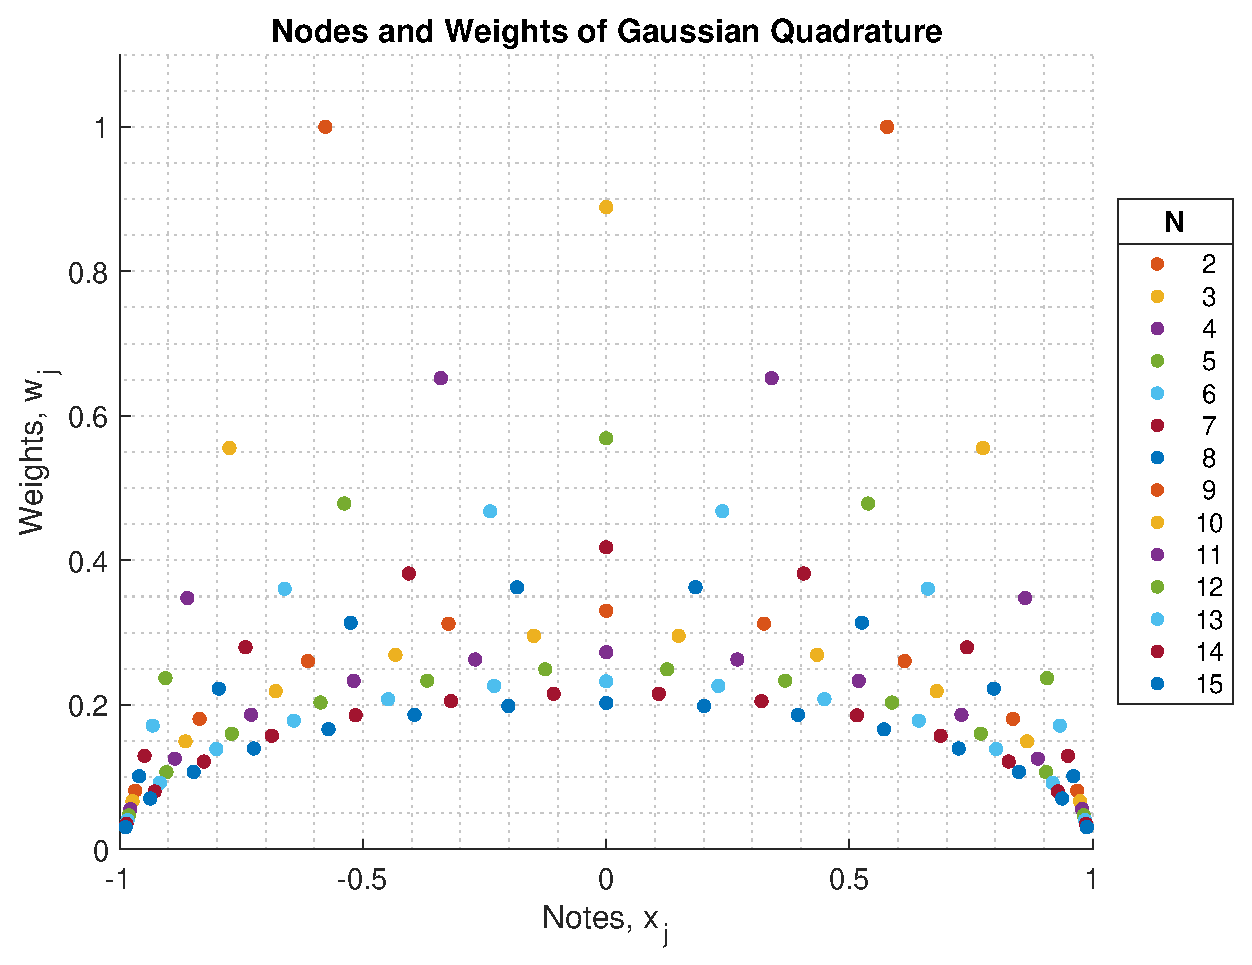
\includegraphics[width=4in]{FastMultipoleMethod/Figures/gaussquad} 
   \caption{Notes and weights of Gaussian quadrature}
   \label{}
\end{figure}

\clearpage
\addtocontents{toc}{\protect\setcounter{tocdepth}{1}}
\subsection{Numerical Integration of Spherical Harmonics}
\addtocontents{toc}{\protect\setcounter{tocdepth}{2}}

Here we derive the number of sampling points needed to numerically integrate spherical harmonics, which follows the results in \cite{darve2000fast}.  Let $f(\theta,\phi)$ be a spherical scalar function composed of a finite number of spherical harmonics
\eq{f(\theta,\phi) = \sum_{l=0}^{L}\sum_{m=-l}^l f_{lm} Y_{lm}(\theta,\phi) \label{fexpansion}}

Integrating this over the unit sphere and separating variables
\ea{\int_0^{2\pi} \int_0^{\pi} f(\theta,\phi) \sin\theta d\theta d\phi  %&=& \sum_{l=0}^{L}\sum_{m=-l}^l f_{lm}  \int_0^{2\pi} \int_0^{\pi} Y_{lm}(\theta,\phi)\sin\theta d\theta d\phi \\
\ & = &  \dfrac{1}{\sqrt{2\pi}}  \sum_{l=0}^{L}\sum_{m=-l}^l  f_{lm}\int_0^{2\pi} e^{im\phi} d\phi \int_0^{\pi}\widetilde P_l^m(\cos\theta) \sin\theta d\theta d\phi \\ }

The integral over $\phi$ can be computed analytically as
\eq{ \int_0^{2\pi} e^{im\phi} d\phi = \begin{cases}
2\pi, \quad \quad m = 0 \\
\dfrac{i (1- e^{2 i \pi m})}{m} = 0, \quad \quad m \ne 0
\end{cases} \label{intphiana} }

It is clear that when $m\ne0$, the double integral will be zero regardless of the value of the $\theta$ integral. We still want to know the number of discrete integration points in $\phi$ required to make this true.  Using trapezoidal integration with periodicity, \eqref{intphiana} is written as a discrete sum over $N$ evenly spaced points
\ea{\int_0^{2\pi} e^{im\phi} d\phi  &=& \Delta \phi \sum_{k=0}^{N-1} e^{im\phi_k}  \\
\ &= & \dfrac{2\pi}{N}  \sum_{k=1}^{N} e^{im k 2\pi/N} \\
\ &= & \dfrac{2\pi}{N}  e^{i(N-1) m \pi/N } \dfrac{\sin(m\pi)}{\sin(m\pi/N)} \label{trapintphi}}

\noindent where $\phi_k = (k-1) \Delta\phi$, $k = 1,...,N$, and $\Delta \phi = 2\pi/N$, The last equation comes from the Dirichlet kernel
\eq{\sum_{k=0}^{N-1} e^{ikx} = e^{i(N-1)x/2} \dfrac{\sin(Nx/2)}{\sin(x/2)}}

\eqref{trapintphi} will be zero when $\vert m \vert < N$, because the numerator sine is zero. When $m = N$, applying L'Hopital's rule, the ratio of sine functions is equal to $N$ while the complex exponent is non-zero. Therefore, the number of samples that correctly integrates all harmonics up to $m = L$ is $N = L + 1$. This can be confirmed numerically and is the same as given in \cite{darve2000fast, beentjes2015quadrature}. We can then write the $\phi$ integral as 
\eq{ \int_0^{2\pi} e^{im\phi} d\phi = \dfrac{2\pi}{L+1} \sum_{i=1}^{L+1} e^{im\phi_i}, \quad 0 \le \vert m \vert \le L }

When $m=0$, the $\theta$ integral becomes 
\ea{ \int_0^{\pi}  P_l(\cos\theta) \sin\theta d\theta &=& - \int_0^{\pi}  P_l(\cos\theta) d\cos\theta \\
\ &=& \int_{-1}^{1}  P_l(\mu) d \mu \\
\ &=& \sum_{j=1}^{N} w_j  P_l(\mu_j) }

with the change of variables $\mu = \cos\theta$ and where the integral has been replaced with Gaussian quadrature. Because $P_l(\mu)$ are polynomials of degree $l$, and because the quadrature is exact for polynomial degrees less than $2n-1$, the number of points that will correctly integrate this is $ l  < 2 n - 1$. For maximum harmonic degree $L$, the number of quadrature nodes is $N = (L+1)/2$, which should be rounded up.  
	
As an aside, when $m$ is even, the associated Legendre polynomials can be integrated with quadrature, because they are simple polynomials. When $m$ is odd, they contain a factor of $\sqrt{1-\mu^2}$, which means they are not simple polynomials, and so cannot be integrated exactly via quadrature. This can be verified numerically. However, analytical integration of $P_l^m(\mu)$ can be done for any $m$, \cite{beentjes2015quadrature,atkinson2012spherical}.


Using these results, numerical integration of a spherical function composed of spherical harmonics with maximum degree $L$ can be computed exactly (to machine precision) as 
\eq{\int_0^{2\pi} \int_0^{\pi} f(\theta,\phi) \sin\theta d\theta d\phi  =   \dfrac{2\pi}{L+1} \sum_{i=1}^{L+1} \sum_{j=1}^{\lceil (L+1)/2 \rceil} w_j f(\theta_j,\phi_i) \label{intsphereharm} }

\noindent where $\phi_i = (i-1)2\pi/(L+1)$, $i = 1,...,L+1$, and $\theta_j = \arccos\mu_j$, where $\mu_j$ and $w_j$ are the nodes and weights of Gaussian quadrature for $\lceil (L+1)/2 \rceil$ points.  

We know that the spherical harmonics are zero-mean over the sphere except the monopole, therefore, if the expansion coefficients are known, one can simply use $f_{00}$ for the mean. If the coefficients are not known, but the function is sampled on the points of quadrature, \eqref{intsphereharm} will compute the mean of $f(\theta,\phi)$ exactly.  

\addtocontents{toc}{\protect\setcounter{tocdepth}{1}}
\subsection{Numerical Integration of Products of Spherical Harmonics}
\addtocontents{toc}{\protect\setcounter{tocdepth}{2}}

Here we derive the number of sampling points needed to numerically integrate a product of spherical harmonics over the unit sphere. This can be done using spherical harmonic synthesis. The expansion coefficients of a scalar spherical function are given by 
\eq{f_{lm} = \int_0^{2\pi} \int_0^{\pi} f(\theta,\phi) Y^*_{lm}(\theta,\phi)\sin\theta d\theta d\phi  }

Substituting \eqref{fexpansion} (ignore for the moment equivalency and orthogonality)
\ea{f_{lm} %&=& \sum_{l'=0}^{L}\sum_{m'=-l'}^{l'} f_{l'm'} \int_0^{2\pi} \int_0^{\pi}  Y_{l'm'}(\theta,\phi)Y^*_{lm}(\theta,\phi)\sin\theta d\theta d\phi \\
&=& \sum_{l'=0}^{L}\sum_{m'=-l'}^{l'} f_{l'm'} \dfrac{1}{2\pi}\int_0^{2\pi} e^{i(m'-m)\phi} d \phi \int_0^{\pi}  \widetilde P_{l'}^{m'}(\cos\theta)  \widetilde P_l^m(\cos\theta)  \sin\theta d\theta \\
 }

Using the reasoning in the previous section, the maximum harmonic in the $\phi$ integration is $2L$. Therefore the number of equally spaced sampling points that are required for trapezoidal integration in $\phi$ is $2L + 1$. The product of two associated Legendre polynomials is a pure polynomial of degree $2L$ for any $m$. Therefore, the number of required samples for Gaussian quadrature in $\theta$ is $\lceil L + 1/2 \rceil$, which can be immediately rounded up to $L + 1$. 

Using these, numerical integration of the product of two spherical 
functions, $f(\theta,\phi)$ and $g(\theta,\phi)$, each with maximum harmonic degree $L$ can be computed exactly as 
\eq{\int_0^{2\pi} \int_0^{\pi} f(\theta,\phi) g(\theta,\phi)  \sin\theta d\theta d\phi =  \dfrac{2\pi}{2L+1} \sum_{i=1}^{2L+1} \sum_{j=1}^{L+1} w_j f(\theta_j,\phi_i)g(\theta_j,\phi_i) \label{intharmprod}}

\noindent where $\phi_i = (i-1)2\pi/(2L+1)$, $i = 1,...,2L+1$, and $\theta_j = \arccos\mu_j$, where $\mu_j$ and $w_j$ are the nodes and weights of Gaussian quadrature for $L + 1$ points.  It is common to find \eqref{intharmprod} in the literature applied to spherical functions without stipulating whether the underlying function is composed of pure harmonics of a product of spherical harmonics.


 \begin{figure}[H] 
   \centering
   \subfigure{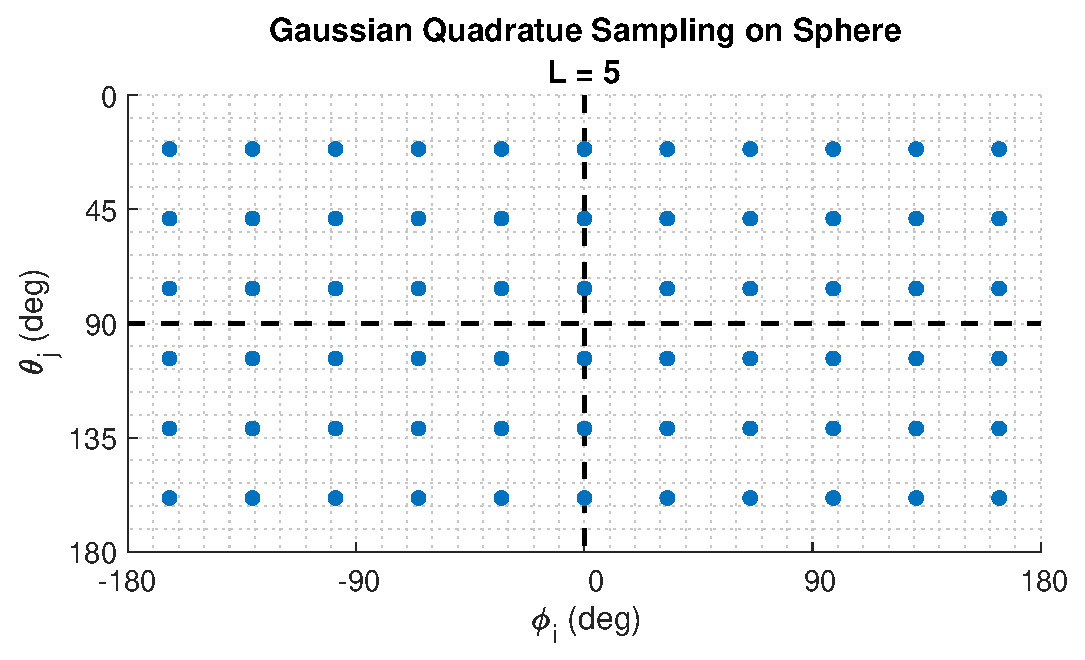
\includegraphics[width=3in]{FastMultipoleMethod/Figures/quadsphere5}}
       \subfigure{\includegraphics[width=3in]{FastMultipoleMethod/Figures/quadsphere6}}
   \caption{Nodes of trapezoidal integration ($\phi_i$) and Gaussian quadrature ($\theta_j$) for integrating products of spherical functions.}
   \label{}
\end{figure}



The nodes $\theta_j$ are almost uniformly spaced, and they never sample the poles because of the nodes of Gaussian quadrature do not sample the end points. This is especially convenient for vector spherical harmonics where the polarization is ambiguous at the poles. When $L+1$ is odd, the nodes will sample the equator. This scheme does crowd the poles somewhat.

Finally, \eqref{intharmprod} can be viewed as computing the power of a field over the sphere when the second function is conjugated (or computing the cross-correlation of two fields). If the spherical harmonic expansion coefficients are known, the analogous form of Parseval's theorem can be used to simply sum the magnitude squared of the coefficients. If the coefficients are not known, \eqref{intharmprod} will compute a power-like quantity exactly from samples of the field(s). 



%
%Integration of a spherical function $f(\hat{\bb{k}})$ over the unit sphere can be written generally as 
%\eq{\int f(\hat{\bb{k}}) d\hat{\bb{k}} = \int_0^{2\pi} \int_0^{\pi} f(\theta,\phi) \sin\theta d\theta d\phi }
%
%\noindent where $\hat{\bb{k}} = (\sin\theta\cos\phi, \sin\theta\sin\phi, \cos\theta)$.  
%
%This integral can be computed exactly from the samples of $f(\hat{\bb{k}})$, if $f$ is band-limited, using a hybrid of Gauss-Legendre quadrature in $\theta$ and trapezoidal integration in $\phi$.  After a change of variables, the integral is 
%\begin{eqnarray}
%\int f(\hat{\bb{k}}) d\hat{\bb{k}} & =& \int_0^{2\pi} \int_0^{\pi} f(\theta,\phi) \sin\theta d\theta d\phi \\
%\ & =& \int_0^{2\pi} \int_{-1}^1 f(\mu,\phi) d\mu d\phi \\
%\ & = & \dfrac{2\pi}{2L+1} \sum_{i=1}^{2L+1} \sum_{j=1}^{L+1} w_j f(\theta_j,\phi_i) \label{sphereint}
%\end{eqnarray}
%
%
%
%
%\noindent where $w_j$ are the weights corresponding to Gaussian nodes $\mu_j$ on $[-1,1]$. The angular sampling points are $\theta_j = \arccos\mu_j$ and $\phi_i = (i-1)2\pi/(2L+1)$. $L$ is the maximum degree required to expand the function $f(\theta,\phi)$ in spherical harmonics.  Interestingly, the nodes $\theta_j$ are almost uniformly spaced, and they never sample the poles because of the nodes of Gaussian quadrature do not sample the end points. When $L+1$ is odd, the nodes will sample the equator.
%
%Address the no-quite polynomials for straight spherical harmonics.   Spherical transforms and green's function contain products of these harmonics. 

\addtocontents{toc}{\protect\setcounter{tocdepth}{1}}
\subsection{Green's Function Integration}
\addtocontents{toc}{\protect\setcounter{tocdepth}{2}}

Following \cite{yucel2008helmholtz}, we give the number of sample points required to correctly integrate the plane wave expansions in the FMM. Using the addition theorem for plane waves 
\eq{e^{i \bb{k}\cdot \bb{d}} = \sum_{l=0}^{\infty} i^l (2l+1) j_l(kd) P_l(\hat{\bb{k}}\cdot\hat{\bb{d}})}

\eqref{fmmexp3} can be written 
\ea{\dfrac{e^{ik\vert \bb{X} + \bb{d} \vert}}{\vert \bb{X} + \bb{d} \vert}  &=& \dfrac{i k}{4\pi}  \sum_{l=0}^{\infty} \sum_{l'=0}^{\infty} i^l (2l+1) i^{l'} (2l'+1) h_l^{(1)}(k X)   j_l'(kd)   \int   P_l(\hat{\bb{k}} \cdot\hat{\bb{X}}) P_l'(\hat{\bb{k}}\cdot\hat{\bb{d}})   d\Omega_k }

Using the addition theorem for Legendre polynomials, 
\eq{P_l(\hat{\br} \cdot \hat{\br}') = \dfrac{4\pi}{2l + 1} \sum_{m=-l}^l Y_{lm}(\theta,\phi) Y_{lm}^*(\theta',\phi')}

the integral can be expanded as 
\eq{\int  P_l(\hat{\bb{k}} \cdot\hat{\bb{X}}) P_l'(\hat{\bb{k}}\cdot\hat{\bb{d}})   d\Omega_k   = \dfrac{4\pi}{2l + 1} \dfrac{4\pi}{2l' + 1}  \sum_{m=-l}^l  \sum_{m=-l'}^{l'} Y_{lm}^*(\theta_X',\phi_X') Y_{lm}^*(\theta_d',\phi_d')    \int  \left(Y_{lm}(\theta_k,\phi_k)\right)^2 d\Omega_k }

Which shows that the spherical integral in \eqref{fmmexp3} is really integrating a product of spherical harmonics. Therefore, using the results from the previous section, the integral over planes waves in the Green's function kernel \eqref{kernelexp} can be computed exactly over discrete values of the wave vector $\hat{\bb{k}}_{ij}$ as 
\eq{ \dfrac{e^{ik\vert \br - \br' \vert}}{\vert \br - \br' \vert}  \approx \dfrac{ik}{4\pi} \dfrac{2\pi}{2L+1} \sum_{i=1}^{2L+1} \sum_{j=1}^{L+1} w_j  e^{ik \hat{\bb{k}}_{ij}\cdot(\br - \br_o)} T_L(k \hat{\bb{k}}_{ij},\bb{X}) e^{-ik \hat{\bb{k}}_{ij} \cdot(\br' - \br_s) } }

which is the result in \cite{yucel2008helmholtz}. The approximation comes from truncating the sum in \eqref{kernelexp}, not the spherical integration.  




\section{Aggregation/Disaggregation}

Here we give a basic idea of how to aggregate, translate, and disaggregate fields in the context of the FMM operations following the explanation in \cite{yucel2008helmholtz}. The routines for computing the translation operator are given in Section \ref{transoperator}, while routines for interpolating and filtering scalar and vector fields are given in Sections \ref{sec:scasphfilter} and \ref{sec:vecsphfilter}.

\addtocontents{toc}{\protect\setcounter{tocdepth}{1}}
\subsection{Octree}
\addtocontents{toc}{\protect\setcounter{tocdepth}{2}}

Typically the scatterers in an FMM problem are organized on a hierarchical octree. An octree is a data structure in which each node has eight children. This is combined with the geometric process of subdividing a cubic volume into eight equal octants. The eight subcubes are called the children of the larger parent cube and visa versa. A cube at every level has an outgoing and incoming far-field pattern associated with it, say $\bb{F}(\hat {\bb{k}})$, which is sampled on the sphere according to the rules of quadrature. This field expansion is centered on the cube and has harmonic bandwidth (i.e., maximum degree vector spherical harmonic, $L$) at least as large as that required for the diameter of the enclosing sphere, and further set by the desired accuracy of the translation operations. This means that fields are coarsely sampled in $(\theta,\phi)$ at higher levels (smaller cubes), and more finely sampled at lower (larger cubes) levels.

Fields are aggregated up the hierarchy, translated at the highest level possible, then disaggregated down the hierarchy. There is a constraint that fields cannot be translated to neighboring boxes at the same level (due to the separation requirement of the translation). This creates a complication when disaggregating. For more details see \cite{yucel2008helmholtz}. In general, aggregation and disaggregation do not have to be restricted to octree structures as long as the bandwidth and separation between the groups of scatterers is obeyed. 


 \begin{figure}[h] 
   \centering
   \includegraphics[width=6in]{FastMultipoleMethod/Figures/aggdiss} 
   \caption{Aggregation, translation, and disaggregation. }
   \label{}
\end{figure}



\addtocontents{toc}{\protect\setcounter{tocdepth}{1}}
\subsection{Aggregation}
\addtocontents{toc}{\protect\setcounter{tocdepth}{2}}

To reiterate, the far pattern of each child cube has lower harmonic content than the parent (due to its smaller size), and therefore coarser spatial sampling in $(\theta,\phi)$. The process of aggregating fields consists of 1) interpolating each far pattern of the children cubes up to the finer sampling of the parent, 2) shifting the phase centers of the children's patterns to that of the parent, then 3) summing the fields of the all the children. The shift is done by multiplication by a complex exponential of plane wave phases, which is equivalent to a diagonal matrix-vector multiply and is trivial to compute. 

Let $\bb{F}_{n,l}(\hat {\bb{k}})$ be the vector field for the $n$th group (cube) at level $l$.  Let $P_{l+1}^{l}$ be the interpolation operator that interpolates a field from level $l+1$ to level $l$. The aggregated field for the $n$th group at the level of the parents is the sum over all interpolated and shifted fields of the children belonging to each parent, \cite{yucel2008helmholtz}:
\begin{equation}
\bb{F}_{n,l}(\hat {\bb{k}}_{l}) = \sum_{m \in G_c} e^{i\bb{k}_{l+1} \cdot (\bb{x}_{n} - \bb{x}_{m}) } P_{l+1}^{l}\left[\bb{F}_{m,l+1}(\hat{ \bb{k}}_{l+1})\right]
\end{equation}

\noindent where $G_c$ are the list of children that belong to parent group $n$, and $\hat {\bb{k}}_{l}$ are the spherical directions sampled for level $l$.

The process of interpolation does not change the harmonic content of the patterns of the children. However, multiplying the pattern by the phase exponential of the plane wave shift is equivalent to convolving the spherical harmonic spectra. This is why the fields are first interpolated, then translated. Another way to think about this is, even though the patterns of the children may contain lower harmonic content when centered on the cubes of the children, the same pattern that is offset from a different center, now belongs to a larger enclosing sphere, and therefore has more harmonic content requiring finer spherical sampling.

\addtocontents{toc}{\protect\setcounter{tocdepth}{1}}
\subsection{Disaggregation}
\addtocontents{toc}{\protect\setcounter{tocdepth}{2}}

Disaggregation sweeps from the lowest level of the octree (largest cubes) to the highest level (smallest cubes) and consists of three steps: 1) shift the field of a parent to the phase center of the child then filter the parent's field to the child's level (i.e., anterpolate), 2) translate the outgoing patterns between groups at the same level that are not near-neighbors but whose parents are near-neighbors (i.e., called the neighborhood of the child), 3) sum the filtered and translated fields. This is done recursively from the bottom level to the top level for all groups and can be written. 
\begin{equation}
\bb{G}_{m,l}(\hat {\bb{k}}_{l}) = P_{l-1}^{l}\left[e^{i\bb{k}_{l-1} \cdot (\bb{x}_{m} - \bb{x}_{n}) }  \bb{G}_{n,l-1}(\hat{ \bb{k}}_{l-1})\right] + \sum_{p \in G_w} T_L({\bb{k}}_{l}, \bb{x}_{m} - \bb{x}_{p}) \bb{F}_{p,l}(\hat {\bb{k}})
\end{equation}

\noindent where $P_{l-1}^{l}$ is the filtering operator that filters the parent's field at level $l-1$ to the child sampling, $m$ is index of the child at level $l$, $n$ is the index of the parent at the parent's level, and $G_w$ is the list children at level $l$ that are well-separated from $m$ (i.e., children that are not near-neighbors, but whose parents are near-neighbors). The purpose of filtering the field of the parent is to reduce its total harmonic content to be of the same degree as that of the child. 


\section{Translation Operator}
\label{transoperator}

\subsection{Basic Translation Operator}
The FMM translation operator is 
\begin{equation}
T_L(\bb{k},\bb{X}) = \sum_{l=0}^L i^l (2l+1) h_l^{(1)} (kX) P_l(\hat{\bb{k}}\cdot\hat{\bb{X}}) 
\end{equation}

\noindent where $\bb{X}$ is the Cartesian vector that points from the origin of the source frame to the origin of the observation frame, $k$ is the complex background wavenumber, $\hat{\bb{k}}$ is the Cartesian wave vector direction, $P_l(x)$ is the Legendre polynomial, and $L$ is the maximum degree of the sum. When computing this, it can be written terms of the dot product $\cos\theta = \hat{\bb{k}}\cdot\hat{\bb{X}}$ in order to externalize the vector computations.
\begin{equation}
T_L(kX,\theta) = \sum_{l=0}^L i^l (2l+1) h_l^{(1)} (kX) P_l(\cos\theta) \label{tltheta}
\end{equation}


 \begin{figure}[h] 
   \centering
   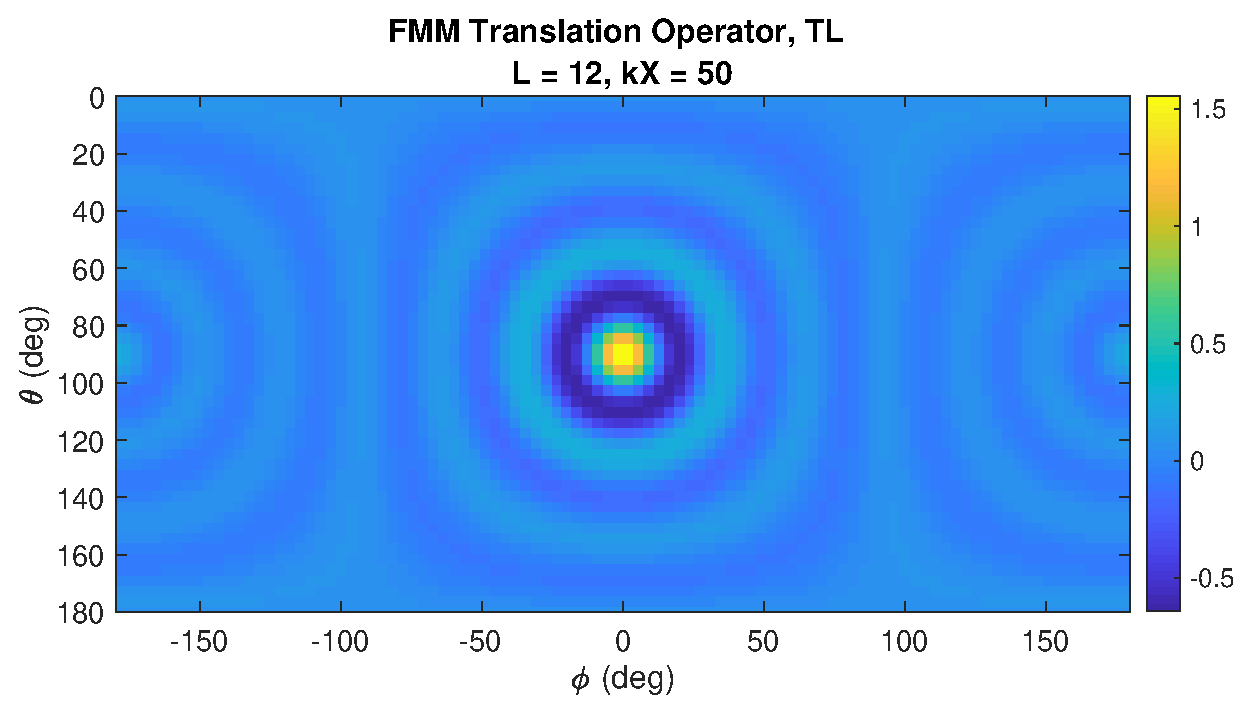
\includegraphics[width=3.5in]{FastMultipoleMethod/Figures/TLtheta} 
   \caption{Real part of the translation operator, \eqref{tltheta}, for $\hat{\bb{X}} = [1, 0, 0]$, $L = 12$, and $kX = 50$. The grid is highly oversampled compared to the sampling required for quadrature integration over the sphere. Note, the operator is peaked in the direction of propagation and contains a 'back lobe'-like feature.}
   \label{}
\end{figure}



The routine \texttt{TLth} returns the translation operator \eqref{tltheta} given scalars $kX$, $L$, and array of $\cos\theta$, which can be any size. To save memory, the Legendre polynomials are computed inline with the recursion \eqref{plrec}.

{\footnotesize
\VerbatimInput{\code/FastMultipoleMethod/TL/TLth.m}
}



%
%
%
%{\footnotesize
%\VerbatimInput{\code/FastMultipoleMethod/TLth.m}
%}
%
%{\footnotesize
%\VerbatimInput{\code/FastMultipoleMethod/TLmem.m}
%}

\subsection{Translation Operator Interpolation}

Computing the translation operator as a straight sum is a computational bottleneck for large problems.  Much work has gone into finding an optimal computation scheme, and the result is a fast interpolator.  The translation operator is precomputed directly at a coarse sampling, after which any value is found by interpolation to a selectable level of error.  Because the translation operator is band limited, it can be computed exactly from the samples using the approximate prolate spheroid (APS) method.  In practice, only a small subset of samples in the vicinity of the interpolation point needs to be used.  

The interpolation formula using APS is given by \cite{bucci1991optimal,yucel2008helmholtz}
\begin{equation}
\widetilde{T}_L(\theta) = \sum_{m = m_o - p + 1}^{m_o + p} T_L(m\Delta\theta)S_N(\theta-m\Delta\theta,\theta_o)D_M(\theta - m \Delta\theta)
\end{equation}

\noindent where $\widetilde{T}_L(\theta)$ is the interpolated translation operator, $D_M(\theta)$ is the periodic sinc function (or Dirichlet kernel), $S_N(\theta,\theta_o)$ is a windowing function, and $T_L(m\Delta\theta)$ are precomputed samples of the translation operator.  The windowing function is given by 
\begin{equation}
S_N(\theta,\theta_o) = \dfrac{R_N(\theta,\theta_o)}{R_N(0,\theta_o)} 
\end{equation}
\begin{equation}
R_N(\theta,\theta_o) = \dfrac{\sinh\left[ (2N+1) \sinh^{-1} \sqrt{\sin^2(\theta_o/2) - \sin^2(\theta/2)}\right]}{\sqrt{\sin^2(\theta_o/2) - \sin^2(\theta/2)}}
\end{equation}

The Dirichlet kernel is given by 
\begin{equation}
D_M(\theta) = \dfrac{\sin\left[(2M+1)\theta/2 \right]}{(2M+1)\sin(\theta/2)}
\end{equation}

In these expressions, $L$ is the truncation degree of the sum and $M=sL$ is the total number of precomputed sampling points where $s$ is the over-sampling ratio and is an integer.  The required sample spacing is $\Delta \theta = 2\pi/(2M+1)$.  This spacing is over a $2\pi$ circumference, even though we only need $\theta = [0, \pi]$.  This comes from the original papers on optimal interpolation over a sphere, but the formulation persists in the literature.  $N = M-L = (s-1)L$ is the number of over-sampling points.  $m_o = \textrm{Int}[\theta/\Delta\theta]$ is the integer index to the left of the interpolation point, where $\textrm{Int}[\cdot]$ is the integer part or floor function.   $\theta_o = p\Delta\theta$ is the width of the interpolation window, where $p$ is the number of samples on each side of the interpolation point.  The choice of $s$ and $p$ is important for maintaining accuracy while minimizing computation.  Good empirical values are $s = 5$, $p= 3$.  

 \begin{figure}[H] 
   \centering
   \includegraphics[width=3in]{FastMultipoleMethod/Figures/indexing} 
   \caption{Sampling and indexing of the interpolation.  Example for $M = 8$, $p = 3$.  $m=0$ corresponds to $\theta = 0$. Note no sample at $\theta=\pi$.}
   \label{fig4}
\end{figure}

Even though we will only interpolate $\theta = [0, \pi]$, we require precomputed samples outside this range when interpolating near the ends.  The translation operator is an even function of $\theta$, therefore, there are two options to obtain the out of bounds points: 1) Only compute sampling points in the range $\theta = [0, \pi]$ and loop the summation index $m$ back on itself if we go beyond the ends, or 2) precompute the necessary values outside of the range, and let the index roam free. We choose the first for simplicity.  

Figure \ref{fig4} illustrates the sample spacing as it relates to the number of sample points as well as the indexing scheme for precomputing points outside the range $\theta = [0, \pi]$.  There are $p-1$ samples to the left of 0, $p$ samples after $\pi$, $M + 2p$ total sample points, and the array index is $I = m + p$, where $m = [0,M]$.  Figure \ref{fig5} shows the interpolator.  

 \begin{figure}[H] 
   \centering
   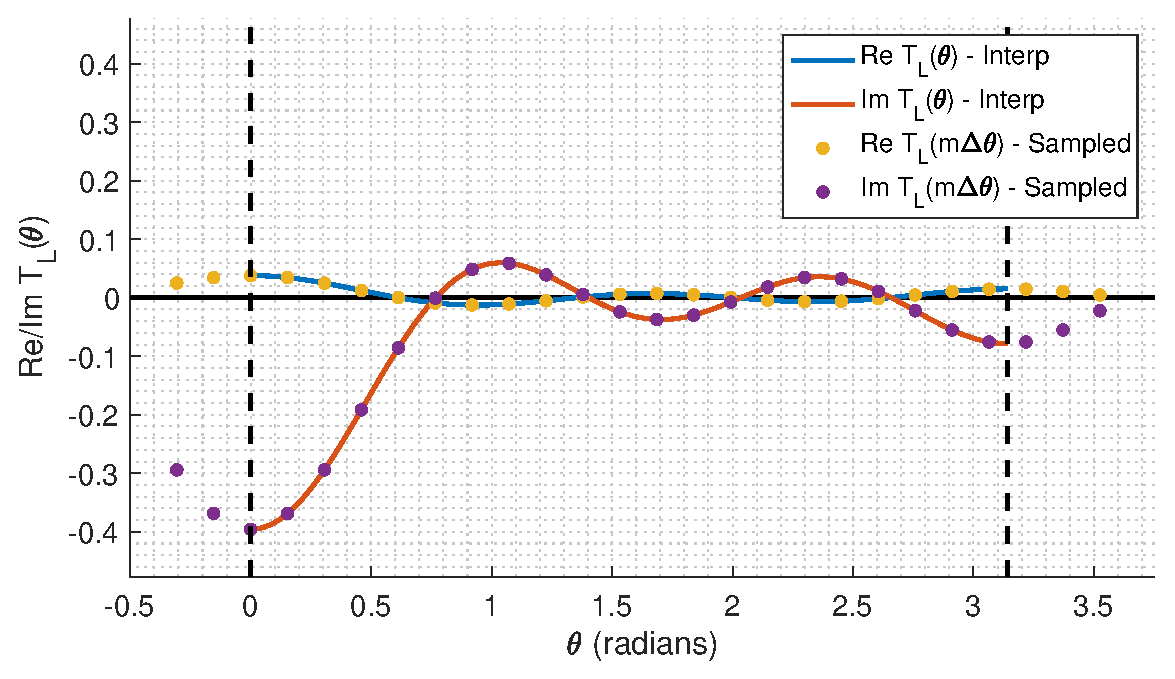
\includegraphics[width=4in]{FastMultipoleMethod/Figures/TLthetainterp} 
   \caption{Translation operator interpolator.  $L = 4$, $s = 5$, $p = 3$, $M = 20$ and there are $M + 2p$ total sampling points.  $k = 2\pi$, $r = 10$. Note there is no sampling point at $\theta = \pi$.}
   \label{fig5}
\end{figure}

The routine \texttt{interpTL} takes as inputs the outputs from the preparatory function \texttt{interpTLprep} as well as the interpolation point(s).  The helper functions are the windowing and Dirichlet kernel, \texttt{SN} and \texttt{DM}.  


{\footnotesize
\VerbatimInput{\code/FastMultipoleMethod/TL/interpTL.m}
}

{\footnotesize
\VerbatimInput{\code/FastMultipoleMethod/TL/interpTLprep.m}
}

{\footnotesize
\VerbatimInput{\code/FastMultipoleMethod/TL/SN.m}
}

{\footnotesize
\VerbatimInput{\code/FastMultipoleMethod/TL/DM.m}
}




\section{Scalar Spherical Filter}
\label{sec:scasphfilter}

In this section, we give routines for interpolating and filtering scalar spherical harmonics following \cite{yucel2008helmholtz}. These routines can stand on their own, because they are excellent for general applications of spherical harmonic expansions. The scalar filters can be used in the scalar form of the FMM for interpolating and filtering fields up and down the multi-level hierarchy structure. These lay the ground work for the vector spherical filters derived later.

\subsection{Spherical Harmonic Transforms}

The spherical harmonics form a complete basis, so any band-limited spherical signal can be represented as a finite sum of harmonics
\begin{equation}
f(\theta,\phi) = \sum_{l=0}^{L} \sum_{m = -l}^{l} f_{lm} Y_{lm}(\theta,\phi)
\label{c6eq1}
\end{equation}

Spherical harmonics can be written in terms of the normalized Legendre polynomials as 
\begin{equation}
Y_{lm}(\theta,\phi) = \dfrac{1}{\sqrt{2\pi}}\widetilde{P}_l^m(\cos \theta)e^{im\phi}
\end{equation}

Using orthogonality of the spherical harmonics, the expansion coefficients are

%\begin{equation}
%\int_{0}^{2\pi} \int_{0}^{\pi} Y_{lm}(\theta,\phi) Y^*_{l'm'}(\theta,\phi) \sin\theta d\theta d\phi = \delta_{ll'}\delta_{mm'}
%\end{equation}

%from which is follows that

\begin{equation}
f_{lm} = \int_{0}^{2\pi} \int_{0}^{\pi}  f(\theta,\phi) Y^*_{l'm'}(\theta,\phi) \sin\theta d\theta d\phi   
\label{c6eq3}
\end{equation}

Equation \eqref{c6eq3} is the forward transform, or spherical harmonic analysis, while equation \eqref{c6eq1} is the inverse transform, or spherical harmonic synthesis.  




\subsection{Forward Scalar Spherical Transform}

Computing \eqref{c6eq3} consists of two steps: 1) forward Fourier transform in $\phi$, 2) forward Legendre transform in $\theta$.  Writing out \eqref{c6eq3}
\begin{equation}
f_{lm} = \int_{0}^{\pi} \widetilde{P}_l^m(\cos \theta) \sin \theta d \theta \dfrac{1}{\sqrt{2\pi}} \int_{0}^{2\pi}   f(\theta,\phi) e^{-im\phi} d\phi   
\end{equation}

\noindent where $\widetilde{P}_l^m(\cos \theta)$ are the fully normalized Legendre polynomials.  The $\phi$ integral is computed first in order to create a set of 1D functions of $\theta$ for each $m$
\begin{equation}
f_m(\theta) = \dfrac{1}{\sqrt{2\pi}} \int_{0}^{2\pi}   f(\theta,\phi) e^{-im\phi} d\phi   
\end{equation}

Evaluating this with trapezoidal integration
\begin{equation}
f_m(\theta) = \dfrac{\sqrt{2\pi}}{I} \sum_{i=1}^{I} f(\theta,\phi_i) e^{-im\phi_i} 
\end{equation}

\noindent where $I$ is the number of grid points in longitude and $\phi_i = 2\pi i/ I $ for $ i = 0,...,I-1$.  This can be computed via FFT. The $\theta$ integral is next computed for each $f_m(\theta)$ by using the forward Legendre transform with a change of variables 
\ea{f_{lm} &=& \int_{0}^{\pi} f_m(\theta) \widetilde{P}_l^m(\cos \theta) \sin \theta d \theta \\
\ & = & -\int_{0}^{\pi} f_m(\theta) \widetilde{P}_l^m(\cos \theta) d\cos\theta \\
\ & = & \int_{-1}^{1} f_m(\theta( \mu)) \widetilde{P}_l^m(\mu) d\mu, \quad \mu = \cos\theta }

%
%\begin{equation}
%f_{lm} = \int_{0}^{\pi} f_m(\theta) \widetilde{P}_l^m(\cos \theta) \sin \theta d \theta 
%\end{equation}
%
%Making a change of variables
%\begin{eqnarray}
%%f_{lm} &=& \int_{0}^{\pi} f_m(\theta) \widetilde{P}_l^m(\cos \theta) \sin \theta d \theta \\
%f_{lm} & = & -\int_{0}^{\pi} f_m(\theta) \widetilde{P}_l^m(\cos \theta) d\cos\theta \\
%%\ & = & \int_{\pi}^{0} f_m(\theta) \widetilde{P}_l^m(\cos \theta) d\cos\theta \\
%\ & = & \int_{-1}^{1} f_m(\theta( \mu)) \widetilde{P}_l^m(\mu) d\mu, \quad \mu = \cos\theta 
%\end{eqnarray}

This can now be evaluated with Gaussian quadrature on the interval $\mu = [-1, 1]$ as
\begin{equation}
f_{lm} = \sum_{j=1}^J f_m(\theta_j) \widetilde{P}_l^m(\mu_j) w_j \label{forwardlegendre}
\end{equation}

\noindent where $J$ is the number of points in latitude and the weights, $w_j$, correspond to the nodes $\theta_j = \arccos\mu_j$.  One first selects the number of grid points in latitude, retrieves the Gaussian nodes for that number of integration points, then evaluates the points $\theta_j$.  Because this operation is integrating products of spherical harmonics, the integral is exact if the number of grid points in latitude and longitude are $J = L+1$ and $I = 2L+1$ for coefficients through $L$. By virtue of the Gaussian quadrature node spacing, the field is never evaluated at the poles.

The routine \texttt{sst} performs the forward scalar spherical transform and returns the spectral coefficients $f_{lm}$.  The coefficients are returned on a 1D array of size $L^2 + 2L + 1$, linearly indexed.  It takes as inputs the maximum degree $L$ for which harmonics are desired. The spherical function $f(\theta_j,\phi_i)$ is sampled on an $I \times J$ meshgrid, where $I = 2L'+1$ and $J = L'+1$ are such that $L' \ge L$.  The sample points need to be $\phi_i = 2\pi i/ I $ for $ i = 0,...,I-1$, and $\theta_j = \arccos \mu_j $, where $\mu_j$ are the $J$ quadrature nodes on $\mu = [-1, 1]$, which are also inputs. In other words, the grid can be sampled more finely than the maximum degree of the harmonics desired for the coefficients. $f_m(\theta_j)$ is computed in place with an FFT along the first dimension of the array.  Matlab's \texttt{fft} produces a two-sided DFT, and $2L+1$ is always odd, so the rows of the matrix $f_m(\theta_j)$ correspond to the spectral components $m = 0, 1, ..., (I-1)/2, -(I-1)/2, ..., -1$.  The rows of the 1D FFT are indexed 
\begin{equation}
\textrm{idx}(I,m) = \left\{ \begin{array}{cc} m + 1, & m \ge 0 \\ I - m + 1, & m < 0 \\ \end{array} \right.
\end{equation}

%Finally, this uses our routine \texttt{Plm} for associated Legendre polynomials, which ensures that one factor of $(-1)^m$ in included in the definition of the spherical harmonics.


%uses onThe Legendre polynomials are computed normalized with Matlab's \texttt{legendre} function and \texttt{'norm'} option.  An extra factor of $(-1)^m$ is included in that definition. Therefore, we need to cancel this to be content with our use of the Condon-Shortly phase that we include in our definition of spherical harmonics.

%
%Note: the definition of Legendre polynomials has a factor of $(-1)^m$.  Our definition of spherical harmonics includes the Condon-Shortly phase, which means there are really two factors of $(-1)^m$ in the entire definition.  Our spherical harmonics are consistent with the wave function translation matrices.  This derivation of the filter does not include the extra $(-1)^m$ on the spherical harmonics, only the one in the definition of the Legendre polynomials, which is also included with the \texttt{'norm'} option.  The filter works was shown to work with just the one factor.  Therefore, we take out the second factor of $(-1)^m$ by multiplying by $(-1)^m$.  If the definition of the the spherical harmonics does not include that phase, then that part of the code should be removed.

{\footnotesize
\VerbatimInput{\code/FastMultipoleMethod/SphericalFilters/sst.m}
}



\subsection{Inverse Scalar Spherical Transform}

The inverse transform consists of taking the expansion coefficients $f_{lm}$ and applying 1) the inverse Legendre transform in $\theta$, 2) the inverse Fourier transform in $\phi$.  The inverse Legendre transform is 

\begin{equation}
f_m(\theta_j) = \sum_{l = \vert m \vert}^{L} f_{lm} \widetilde{P}_l^m(\mu_j)
\label{eqist1}
\end{equation}

\noindent where again $\mu_j = \cos\theta_j$.  The inverse Fourier transform in $\phi$ is

\begin{equation}
f(\theta_j,\phi_i) = \dfrac{1}{\sqrt{2\pi}}\sum_{m = -L}^{L} f_m(\theta_j) e^{im\phi_i}
\label{eqist2}
\end{equation}

The routine \texttt{isst} computes the inverse scalar spherical transform.  The inputs are the array of harmonics $f_{lm}$ of size $L^2 + 2L + 1$ linearly indexed, and the maximum degree $L$. It then returns the $I \times J$ spherical function $f(\theta_j,\phi_i)$ as a meshgrid such that $I = 2L'+1$ and $J = L' + 1$, where $\phi_i = 2\pi i/ I $ for $ i = 0,...,I-1$, and $\mu_j = \cos\theta_j$.  $J$ is determined by the length of the input $\mu_j$, which can be larger than the corresponding sampling of the $L$ harmonics in $f_{lm}$ (this allows the routine to preform interpolation automatically). An additional factor of $I$ is needed because Matlab's \texttt{ifft} divides by the number of samples in $\phi$.  

{\footnotesize
\VerbatimInput{\code/FastMultipoleMethod/SphericalFilters/isst.m}
}

\clearpage

\subsection{Scalar Spherical Filter}

The forward and inverse scalar spherical transforms can be used together to accomplish interpolation or filtering (anterpolation) of a spherical function.  

Interpolation takes a function $f(\theta,\phi)$ with coarse sampling and $L$ harmonics, and upsamples it to a function $f(\theta',\phi')$ with finer sampling and $K$ harmonics, where $K > L$.  Because the original signal is band limited with maximum harmonic $L$, the interpolated signal contains the same harmonic content, and is interpolated exactly. This is the spherical harmonic analog of upsampling a Nyquist-sampled exactly to an arbitrarily fine sampling with sinc interpolation.  Interpolation is accomplished by first computing the spectral components $f_{lm}$ of $f(\theta,\phi)$ using the scalar spherical transform to degree $L$, zero-padding the coefficients to degree $K$ to form $f_{lm}'$, then applying the inverse scalar spherical transform to create $f(\theta',\phi')$.

Filtering takes $f(\theta',\phi')$ with fine sampling and $K$ harmonics to a function $f(\theta,\phi)$ with coarse sampling and $L$ harmonics, where $L < K$.  This is analogous to filtering a signal and resampling it at lower rate.  Filtering necessarily eliminates higher frequency harmonics.  Filtering is accomplished by computing the spectral components $f_{lm}'$ of $f(\theta',\phi')$ via the SST to degree $K$, truncating down to degree $L$ to form $f_{lm}$, then applying the ISST to create $f(\theta,\phi)$.

\begin{equation}
\begin{array}{cccccccccc}
\textrm{Interpolation:} & f(\theta,\phi) & \stackrel{\textrm{sst}}{\rightarrow} & f_{lm}, L & \rightarrow & \textrm{zero pad} &\rightarrow & f_{lm}', K & \stackrel{\textrm{isst}}{\rightarrow} & f(\theta',\phi') \nonumber \\
\textrm{Filter:} & f(\theta',\phi') & \stackrel{\textrm{sst}}{\rightarrow} & f_{lm}', K & \rightarrow & \textrm{trunctate} &\rightarrow & f_{lm}, L &\stackrel{\textrm{isst}}{\rightarrow} & f(\theta,\phi) \nonumber \\
\end{array}
\end{equation}

%
% \begin{figure}[h] 
%   \centering
%   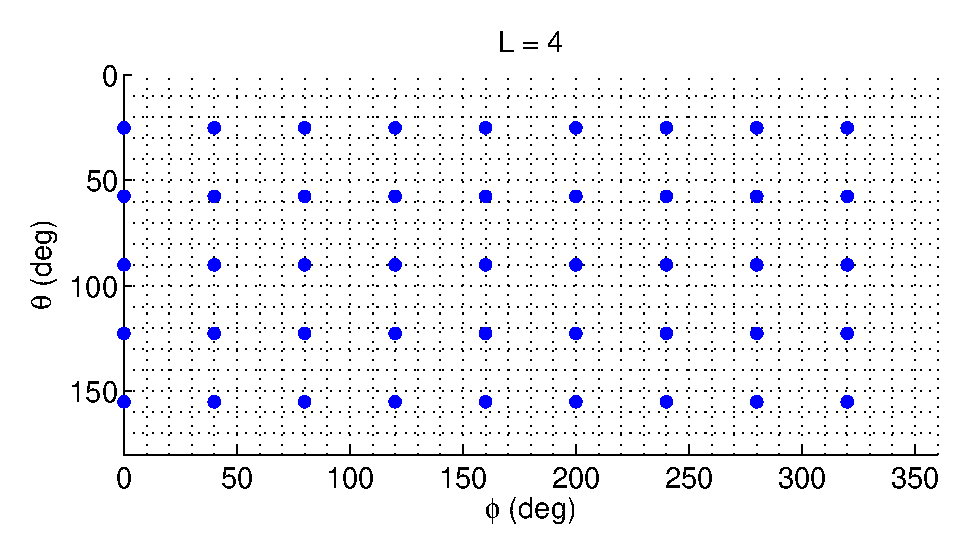
\includegraphics[width=3.5in]{FastMultipoleMethod/Figures/samples} 
%   \caption{Sample spacing for $L = 4$.}
%   \label{}
%\end{figure}
%


 \begin{figure}[H] 
 \centering
\subfigure{
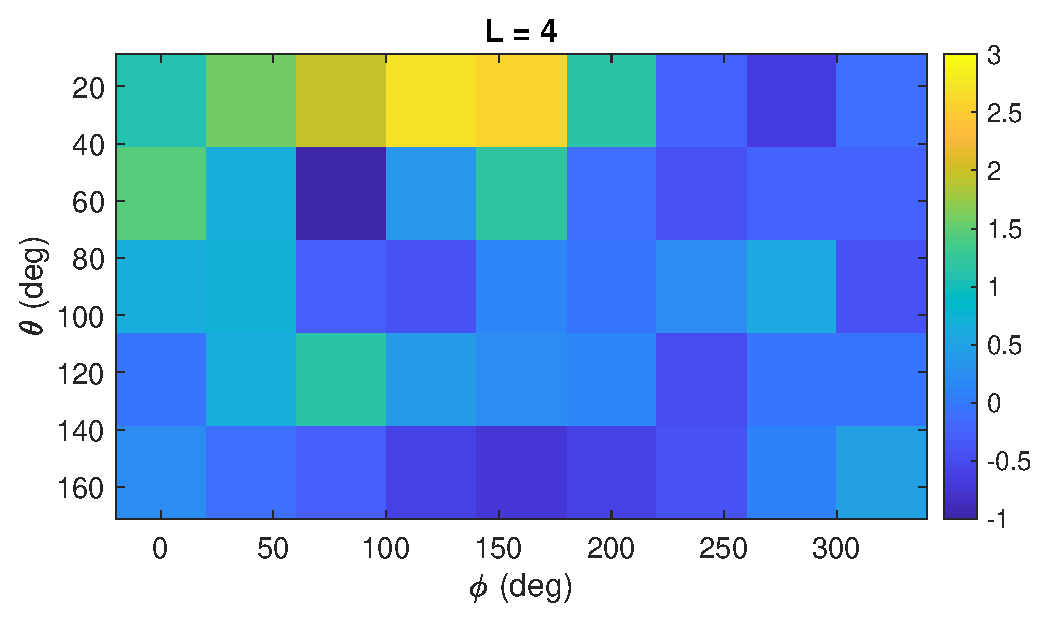
\includegraphics[width=3in]{FastMultipoleMethod/Figures/filt1} } 
\subfigure{
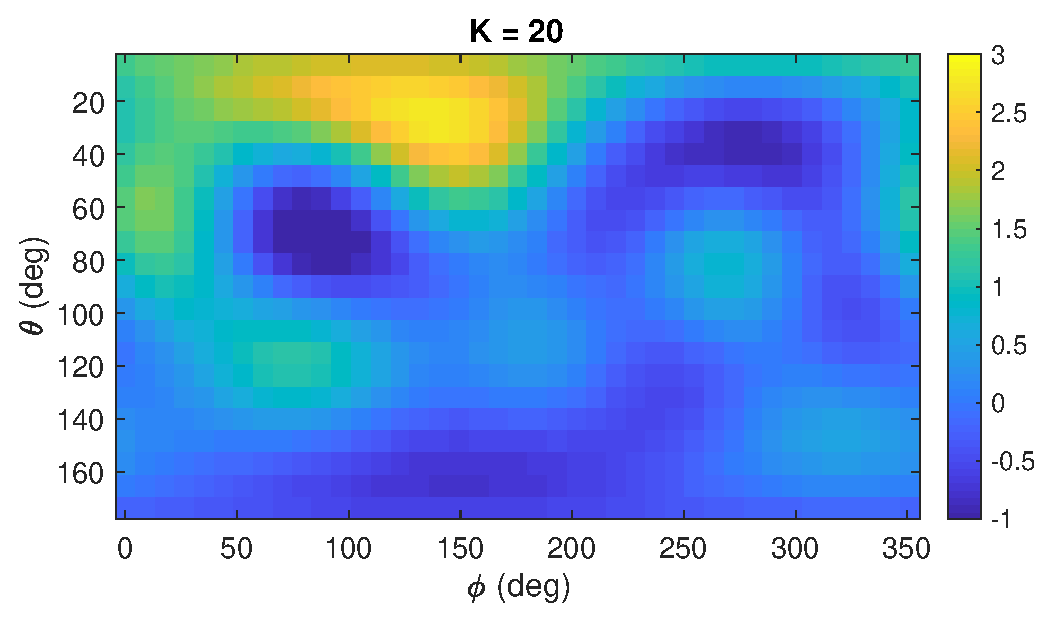
\includegraphics[width=3in]{FastMultipoleMethod/Figures/filt2} } 
\caption{Interpolation of a complex scalar field (real part). Left: coarsely sampled field. Right: finely sampled interpolated field. }
\end{figure}

 \begin{figure}[H] 
 \centering
\subfigure{
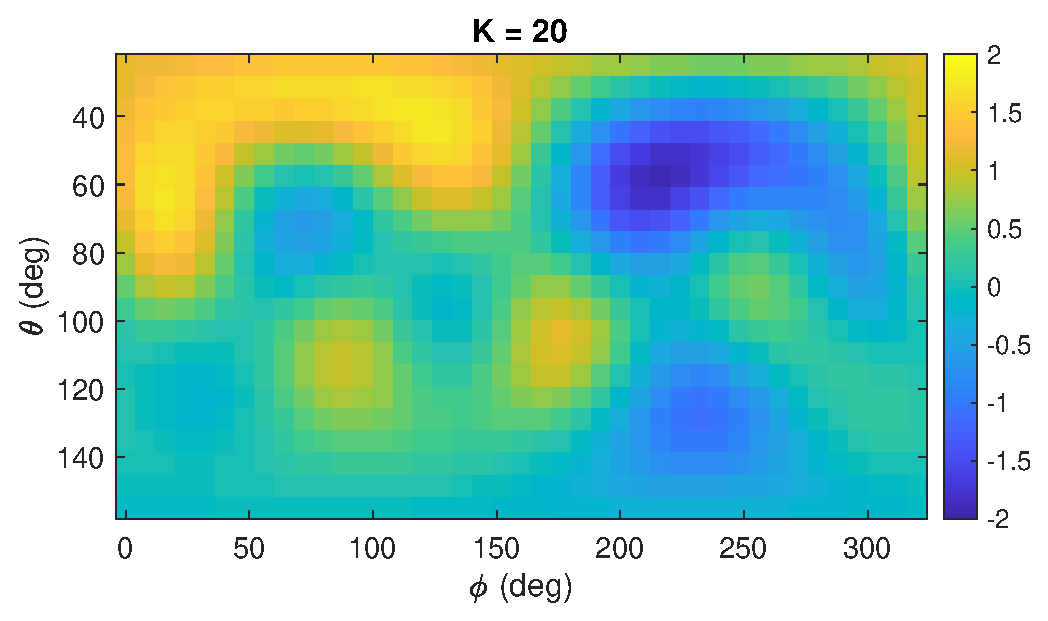
\includegraphics[width=3in]{FastMultipoleMethod/Figures/filt3} } 
\subfigure{
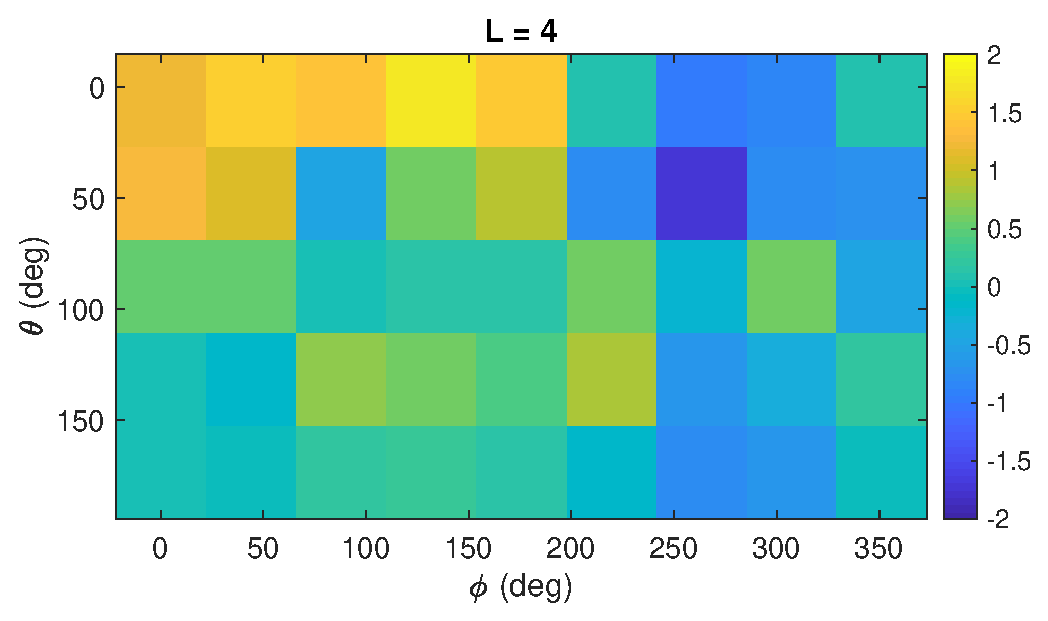
\includegraphics[width=3in]{FastMultipoleMethod/Figures/filt4} } 
\caption{Filtering of a complex scalar field (real part). Left: finely sampled field. Right: coarsely sampled filtered field. }
\end{figure}


The routine \texttt{ssfilt} computes the scalar spherical interpolation or filtering operation.  It takes the maximum harmonic degrees $L$ and $K$, where $L \le K$.  The harmonic content is either interpolated from $L$ to $K$ or filtered from $K$ to $L$.  For interpolation, the input function is $f(\theta,\phi)$, sized $2L'+1 \times L' + 1$ on a meshgrid, and the routine returns $f(\theta',\phi')$, sized $2K'+1 \times K'+1$, where $L'$ and $K'$ are set by the length of $\mu_j$ and $\mu_k$, respectively.  The sampling of the grid can have more harmonics than the interpolation/filter harmonics. As always, it assumes $\phi$ is uniformly spaced and $\theta$ is spaced according to the Gaussian quadrature nodes.  This routine calls \texttt{sst} and \texttt{isst} that recompute the underlying Legendre polynomials at each run and is not built for speed.  

{\footnotesize
\VerbatimInput{\code/FastMultipoleMethod/SphericalFilters/ssfilt.m}
}

\clearpage

\subsection{Fast Scalar Spherical Filter}
\label{sec:fastscasphfilt}
The bottle neck of the scalar spherical filter lies in the sums of the forward and inverse Legendre transforms, especially when $L$ is large.  The fix is to combine the two transforms, after which the sums can be simplified and further accelerated with the 1D FMM, which is described in Section \ref{sec:1dfmm}. For a discussion of the computational complexity, see \cite{yucel2008helmholtz}.

Assume that interpolation is being done and $L < K$.  The quantities $\theta_j$, $\mu_j$, and $w_j$ are associated with $L$ harmonics of field $f(\theta_j,\phi_i)$, and the quantities $\theta_k$, $\mu_k$, and $w_k$ are associated with $K$ harmonics of field $f'(\theta_k,\phi_k)$ and the routine is interpolating $f(\theta_j,\phi_i)$ to $f'(\theta_k,\phi_k)$. Start by substituting the forward Legendre transform, \eqref{forwardlegendre}, into the inverse Legendre transform, \eqref{eqist1}, 
\begin{equation}
f_m'(\theta_k) = \sum_{l = \vert m \vert}^{K} \left(\sum_{j=1}^J f_m(\theta_j)\widetilde{P}_l^m(\mu_j)w_j\right) \widetilde{P}_l^m(\mu_k)
\end{equation}

When $L<K$, the sum over $K$ can be restricted to $L$ because $f_m(\theta_j)$ does not have harmonics when $\vert m\vert> L$.  This is equivalent to zero-padding the harmonics $f_{lm}$ in the standard spherical filter. Changing the limit of the sum and exchanging the order of the sums
\begin{equation}
f_m'(\theta_k) = \sum_{j=1}^J f_m(\theta_j)w_j \sum_{l = \vert m \vert}^{L} \widetilde{P}_l^m(\mu_j) \widetilde{P}_l^m(\mu_k) \label{combineLtrans}
\end{equation}

%\begin{equation}
%f_m'(\theta_k) = \sum_{l = \vert m \vert}^{L} \left(\sum_{j=1}^J f_m(\theta_j)\widetilde{P}_l^m(\mu_j)w_j\right) \widetilde{P}_l^m(\mu_k)
%\end{equation}


The sum over $L$ can be simplified with the Christoffel-Darboux formula 
\begin{equation}
\sum_{l = \vert m \vert}^{L} \widetilde{P}_l^m(\mu_j) \widetilde{P}_l^m(\mu_k) = \epsilon_{L+1}^m \dfrac{ \widetilde{P}_{L+1}^m(\mu_k)  \widetilde{P}_L^m(\mu_j) - \widetilde{P}_{L}^m(\mu_k)  \widetilde{P}_{L+1}^m(\mu_j)}{\mu_k - \mu_j} \label{cdform}
\end{equation}

where
\begin{equation}
\epsilon_{l}^m  = \sqrt{\dfrac{l^2 - m^2}{4l^2 - 1}}
\end{equation}

Substituting \eqref{cdform} into \eqref{combineLtrans} and separating terms
%\begin{equation}
%f_m'(\theta_k) = \sum_{j=1}^J f_m(\theta_j)w_j\epsilon_{L+1}^m \dfrac{\widetilde{P}_{L+1}^m(\mu_k) \widetilde{P}_{L}^m(\mu_j) - \widetilde{P}_{L}^m(\mu_k) \widetilde{P}_{L+1}^m(\mu_j)}{\mu_k - \mu_j}
%\end{equation}
%
%Separating the terms
\begin{equation}
\dfrac{f_m'(\theta_k)}{\epsilon_{L+1}^m} = \widetilde{P}_{L+1}^m(\mu_k)\sum_{j=1}^J \dfrac{f_m(\theta_j)w_j\widetilde{P}_L^m(\mu_j)}{\mu_k - \mu_j}   - \widetilde{P}_{L}^m(\mu_k)\sum_{j=1}^J \dfrac{f_m(\theta_j)w_j\widetilde{P}_{L+1}^m(\mu_j)}{\mu_k - \mu_j}  \label{cdform2}
\end{equation}

This has the form of a matrix-vector multiply over the kernel of type $1/(x-x')$, therefore it is possible to use the 1D FMM to accelerate this computation. 

When the sum rolls over the case $\mu_k = \mu_j$, L'Hopital's rule can be applied to either $\mu_k$ or $\mu_j$ to resolve the singularity. The condition $\mu_k = \mu_j$ only ever occurs at $\mu = 0$, because the nodes of quadrature for different degrees of harmonics never overlap expect at $\mu = 0$, and only when the number of quadrature points in $\theta$ of both functions is odd. Assuming the number of quadrature points is equal to $L+1$ and $K+1$, this means that the rule needs to be applied when both $L$ and $K$ are even and different (when $L=K$ there is nothing to interpolate or filter). It is possible to avoid the singularity entirely by requiring that $L$ and $K$ always be odd, then $\mu_j \ne \mu_k$ and the Legendre derivative are not needed, but this is too restrictive.  Applying L'Hopital's rule to $\mu_j$ we get a version of \eqref{cdform2} that handles the singularity
\ea{
\dfrac{f_m'(\theta_k)}{\epsilon_{L+1}^m}  &=&
\widetilde{P}_{L+1}^m(\mu_k)\sum_{j=1}^J f_m(\theta_j)w_j
\left\{
\begin{array}{cc}
\dfrac{\widetilde{P}_L^m(\mu_j)}{\mu_k - \mu_j} & \mu_j \ne \mu_k \\
-\dfrac{d\widetilde{P}_{L}^m(\mu_j)}{d\mu_j}  & \mu_j = \mu_k \\
\end{array} \right. 
\nonumber \\
\ & \ & - \widetilde{P}_{L}^m(\mu_k)\sum_{j=1}^J f_m(\theta_j)w_j
\left\{  
\begin{array}{cc}
\dfrac{\widetilde{P}_{L+1}^m(\mu_j)}{\mu_k - \mu_j} & \mu_j \ne \mu_k \\
-\dfrac{d\widetilde{P}_{L+1}^m(\mu_j)}{d\mu_j}  & \mu_j = \mu_k \\
\end{array} \right. }


%
%\begin{eqnarray}
%\dfrac{f_m'(\theta_k)}{\epsilon_{K+1}^m}  &=& \widetilde{P}_{K+1}^m(\mu_k)\sum_{\substack{j=1 \\ \mu_k \ne \mu_j}}^J \dfrac{f_m(\theta_j)w_j\widetilde{P}_K^m(\mu_j)}{\mu_k - \mu_j}   - \widetilde{P}_{K}^m(\mu_k)\sum_{\substack{j=1 \\ \mu_k \ne \mu_j}}^J \dfrac{f_m(\theta_j)w_j\widetilde{P}_{K+1}^m(\mu_j)}{\mu_k - \mu_j} \nonumber \\
%\ & \ & + \left[\dfrac{d\widetilde{P}_{K+1}^m(\mu_k)}{d\mu_k} f_m(\theta_j)w_j\widetilde{P}_K^m(\mu_k)   - \dfrac{d\widetilde{P}_{K}^m(\mu_k)}{d\mu_k}f_m(\theta_j)w_j\widetilde{P}_{K+1}^m(\mu_k)\right]_{\mu_k = \mu_j}
%\end{eqnarray}


%
%\begin{equation}
%\begin{array}{c}
%\dfrac{f_m'(\theta_k)}{\epsilon_{L+1}^m}  =  
%\dfrac{d\widetilde{P}_{L+1}^m(\mu_k)}{d\mu_k}\sum_{j=1}^J f_m(\theta_j)w_j
%\widetilde{P}_L^m(\mu_j) \left\{  
%\begin{array}{cc}
%\dfrac{1}{\mu_k - \mu_j} & \mu_j \ne \mu_k \\
%1  & \mu_j = \mu_k \\
%\end{array} \right.  \\
%-
%\dfrac{d\widetilde{P}_{L}^m(\mu_k)}{d\mu_k}\sum_{j=1}^J f_m(\theta_j)w_j
%\widetilde{P}_{L+1}^m(\mu_j) \left\{  
%\begin{array}{cc}
%\dfrac{1}{\mu_k - \mu_j} & \mu_j \ne \mu_k \\
%1  & \mu_j = \mu_k \\
%\end{array} \right. \\
%\end{array}
%\end{equation}
%
%%\dfrac{f_m(\theta_j)w_j\widetilde{P}_K^m(\mu_j)}{\mu_k - \mu_j}   - \widetilde{P}_{K}^m(\mu_k)\sum_{\substack{j=1 \\ \mu_k \ne \mu_j}}^J \dfrac{f_m(\theta_j)w_j\widetilde{P}_{K+1}^m(\mu_j)}{\mu_k - \mu_j} \nonumber \\
%%\ & \ & + \left[\dfrac{d\widetilde{P}_{K+1}^m(\mu_k)}{d\mu_k} f_m(\theta_j)w_j\widetilde{P}_K^m(\mu_k)   - \dfrac{d\widetilde{P}_{K}^m(\mu_k)}{d\mu_k}f_m(\theta_j)w_j\widetilde{P}_{K+1}^m(\mu_k)\right]_{\mu_k = \mu_j}
%%\end{eqnarray}
%
%
%%\noindent where
%%
%%\begin{equation}
%%\dfrac{d}{dx}\widetilde{P}_{l}^m(x)  = -m \dfrac{x}{1-x^2} \widetilde{P}_{l}^m(x) + \dfrac{\sqrt{(l+m+1)(l-m)}}{\sqrt{1-x^2}} \widetilde{P}_{l}^{m+1}(x)
%%\end{equation}
%%
%%or 
%
%%\begin{equation}
%%\dfrac{d}{dx}\widetilde P_l^m(x) = \dfrac{1}{x^2-1}\left( lx \widetilde P_l^m(x) - \sqrt{\dfrac{(l+1/2)}{(l-1/2)}}\sqrt{(l+m)(l-m)} \widetilde P_{l-1}^m(x)\right)
%%\end{equation}
%
%
%\begin{equation}
%\dfrac{f_m'(\theta_k)}{\epsilon_{L+1}^m}  =  
%\dfrac{d\widetilde{P}_{L+1}^m(\mu_k)}{d\mu_k} \sum_{j=1}^J f_m(\theta_j)w_j \widetilde{P}_L^m(\mu_j) -
%\dfrac{d\widetilde{P}_{L}^m(\mu_k)}{d\mu_k} \sum_{j=1}^J f_m(\theta_j)w_j\widetilde{P}_{L+1}^m(\mu_j), \qquad \mu_k = \mu_j
%\end{equation}

Another way to think about the singular point, when it occurs, is to consider $1/(\mu_k - \mu_j)$ as a matrix that is multiplied on the right by a vector that indexes $\mu_j$ (e.g., $f_m(\theta_j) w_j\widetilde P_L^m(\mu_j)$) and multiplied element-wise on the left by a vector that indexes $\mu_k$ (e.g., $\widetilde P_L^m(\mu_k)$).  Only the central matrix element needs to be adjusted, but the adjustment applies to both the matrix element and the element in the right hand vector. This makes what should be a simple matrix-vector multiply awkward to compute. We handle this by recomputing the row-vector multiplication that contains the singular point separately, but better solutions exist.  Finally, the application of L'Hopital's rule in \cite{yucel2008helmholtz} does not appear to handle the sum over $j$ correctly, and \cite{jakob1997fast} mentions this procedure but does not give the equations.

The above equations are for interpolation. For filtering, simply exchange the nodes and weights between $L$ and $K$. The intermediate sum will be restricted again to a maximum degree $L$, because the filtered field only has harmonics up to order $m = L$. Truncating the intermediate sum is equivalent to truncating the coefficients $f_{lm}'$ in the standard spherical filter.   

\subsubsection{Basic implementation}

The routine \texttt{fssfilt} implements a basic version of the fast scalar spherical filter and works the same as \texttt{ssfilt}. It expects $L \le K$ and that the input field be sampled at the nodes of quadrature with either $I = 2L' + 1$ and $J = L' +1$ points for interpolation, or $P = 2K' +1$ and $Q = K' + 1$ points for filtering. $L'$ and $K'$ are set by the length of $\mu_j$ and $\mu_k$, respectively, such that $L' \ge L$ or $K' \ge K$.  Provisions are included for the singular point based on the values of $L'$ and $K'$. It computes the matrix-vector multiplication directly and does not implement the 1D FMM acceleration. It also computes the Legendre polynomials anew at each call, so it can be made much faster with appropriate precomputation, because only the $L$ and $L+1$ harmonics are needed. The routine returns the same result as \texttt{ssfilt} to machine precision, and is several times faster for low number of harmonics.

{\footnotesize
\VerbatimInput{\code/FastMultipoleMethod/SphericalFilters/fssfilt.m}
}

%\subsubsection{Fast implementation}
%
%The real speed of the fast scalar filter comes from using the 1D FMM to accelerate the matrix vector multiplication as well as precomputing the Legendre polynomials and auxiliaries of the 1D FMM.  

\clearpage
\section{Vector Spherical Filter}
\label{sec:vecsphfilter}


In this section, we give routines for interpolating and filtering vector spherical harmonics. Like the scalar routines, they could also stand on their own apart from the FMM. Fast versions of the vector spherical filter are also possible, either based on similar concepts of the fast scalar filter in which the forward and inverse Legendre transforms are compressed, or by using the fast scalar filter with modifications.
 
\subsection{Vector Spherical Harmonic Transforms}

The vector spherical harmonics form a complete basis, so any band limited vector field can be represented as sum of harmonics
\begin{eqnarray}
\bb{F}(\theta,\phi) &=& F_{\theta}(\theta,\phi) \hat\theta + F_{\phi}(\theta,\phi) \hat\phi \\
\ & = & \sum_{l=1}^{L} \sum_{m = -l}^{l} b_{lm} \bb{B}_{lm}(\theta,\phi) + c_{lm} \bb{C}_{lm}(\theta,\phi)
\end{eqnarray}

\noindent where $F_{\theta}(\theta,\phi)$ and $F_{\phi}(\theta,\phi)$ are scalar spherical functions representing each vector component. In general, the vector spherical harmonics, $\bb{B}_{lm}$ and $\bb{C}_{lm}$, could be fully normalized or partially normalized. Eventually, the fast vector spherical filter will use the fast scalar filter and, to accommodate this, it is best to use the partially normalized vector spherical harmonics in the derivations that follow (as opposed to the fully normalized versions that include a factor of $1/\sqrt{l(l+1)}$). The scalar functions are expanded as
\begin{eqnarray}
 F_{\theta}(\theta,\phi) &=&  \sum_{l=1}^{L} \sum_{m = -l}^{l} b_{lm}  \dfrac{d}{d\theta} Y_{lm}(\theta,\phi)   + c_{lm} \dfrac{im}{\sin\theta} Y_{lm}(\theta,\phi) \label{fmmFtheta} \\
F_{\phi}(\theta,\phi) &=&\sum_{l=1}^{L} \sum_{m = -l}^{l} b_{lm} \dfrac{im}{\sin\theta} Y_{lm}(\theta,\phi) -c_{lm} \dfrac{d}{d\theta} Y_{lm}(\theta,\phi)    \label{fmmFphi}
\end{eqnarray}

which show the mixing of harmonics between vector components.

%\begin{eqnarray}
% F_{\theta}(\theta,\phi) &=&  \sum_{l=1}^{L} \sum_{m = -l}^{l} b_{lm} \dfrac{1}{\sqrt{l(l+1)}} \dfrac{d}{d\theta} Y_{lm}(\theta,\phi)   + c_{lm} \dfrac{1}{\sqrt{l(l+1)}} \dfrac{im}{\sin\theta} Y_{lm}(\theta,\phi)   \nonumber \\
% \ & \ & \ \\
%F_{\phi}(\theta,\phi) &=&\sum_{l=1}^{L} \sum_{m = -l}^{l} b_{lm}  \dfrac{1}{\sqrt{l(l+1)}} \dfrac{im}{\sin\theta} Y_{lm}(\theta,\phi) -c_{lm} \dfrac{1}{\sqrt{l(l+1)}} \dfrac{d}{d\theta} Y_{lm}(\theta,\phi)     \nonumber \\
% \ & \ & \ 
%\end{eqnarray}


The orthogonality relations for these partially normalized vector spherical harmonics are 
\ea{
\int_0^{2\pi} \int_0^{\pi}
\left\{
\begin{array}{c}
\bb{B}_{lm}(\theta,\phi) \cdot \bb{B}^*_{lm}(\theta,\phi) \\
\bb{C}_{lm}(\theta,\phi) \cdot \bb{C}^*_{lm}(\theta,\phi) 
\end{array}
\right\}
\sin\theta d\theta d\phi &=& l(l+1)\delta_{ll'}\delta_{mm'} \\
\int_0^{2\pi} \int_0^{\pi}
\left\{
\begin{array}{c}
\bb{B}_{lm}(\theta,\phi) \cdot \bb{C}^*_{lm}(\theta,\phi) \end{array}
\right\}
\sin\theta d\theta d\phi &=& 0
}

Given a vector field $\bb{F}(\theta,\phi)$, the coefficients are found with
\begin{equation}
\left\{
\begin{array}{c}
b_{lm} \\
c_{lm} \\
\end{array}
\right\}
=
\dfrac{1}{l(l+1)}\int_0^{2\pi} \int_0^{\pi}
\bb{F}(\theta,\phi) \cdot 
\left\{\begin{array}{c}
\bb{B}^*_{lm}(\theta,\phi) \\
\bb{C}^*_{lm}(\theta,\phi) 
\end{array}\right\}
\sin\theta d\theta d\phi \label{vecanalysis}
\end{equation}


\subsection{Forward Vector Spherical Transform}

The forward vector spherical transform, as in the scalar case, is composed of a forward Fourier transform and forward Legendre transform.  Writing out \eqref{vecanalysis}

\begin{eqnarray}
b_{lm} &=& \dfrac{1}{l(l+1)}\int_0^{2\pi} \int_0^{\pi} \dfrac{1}{\sqrt{2\pi}} \left( F_{\theta}(\theta,\phi) \dfrac{\partial \widetilde{P}_l^m(\cos\theta)}{\partial\theta} e^{-im\phi} \right) \sin\theta d\theta d\phi \nonumber \\
\ & \ & + \dfrac{1}{l(l+1)}\int_0^{2\pi} \int_0^{\pi} \dfrac{1}{\sqrt{2\pi}} \left( F_{\phi}(\theta,\phi) \dfrac{(-im)}{\sin\theta} \widetilde{P}_l^m(\cos\theta) e^{-im\phi} \right) \sin\theta d\theta d\phi 
\end{eqnarray}

\begin{eqnarray}
c_{lm} &=& \dfrac{1}{l(l+1)}\int_0^{2\pi} \int_0^{\pi} \dfrac{1}{\sqrt{2\pi}} \left( F_{\theta}(\theta,\phi) \dfrac{(-im)}{\sin\theta} \widetilde{P}_l^m(\cos\theta) e^{-im\phi} \right) \sin\theta d\theta d\phi \nonumber \\
\ & \ & - \dfrac{1}{l(l+1)}\int_0^{2\pi} \int_0^{\pi} \dfrac{1}{\sqrt{2\pi}} \left( F_{\phi}(\theta,\phi)\dfrac{\partial \widetilde{P}_l^m(\cos\theta)}{\partial\theta}  e^{-im\phi} \right) \sin\theta d\theta d\phi 
\end{eqnarray}

The integrals over latitude and longitude can be separated.  Performing the $\phi$ integral first we have 

\begin{eqnarray}
\left\{
\begin{array}{c}
f_{\theta,m}(\theta) \\
f_{\phi,m}(\theta) \\
\end{array}
\right\}
&=&
\dfrac{1}{\sqrt{2\pi}} 
\int_0^{\pi}
\left\{
\begin{array}{c}
F_{\theta}(\theta,\phi) \\
F_{\phi}(\theta,\phi) 
\end{array}\right\}
e^{-im\phi} d\phi  \\
\ &=&
\dfrac{\sqrt{2\pi}}{I}
\sum_{i=1}^I
\left\{
\begin{array}{c}
F_{\theta}(\theta,\phi_i) \\
F_{\phi}(\theta,\phi_i) 
\end{array}\right\}
e^{-im\phi_i} 
\end{eqnarray}

\noindent where the grid points are $\phi_i = 2\pi i/I$ for $i = 0,...,I-1$.  These are evaluated with a fast Fourier transform.  The coefficients are then written in terms of $f_{\theta,m}(\theta)$ and $f_{\phi,m}(\theta)$ as

\begin{eqnarray}
b_{lm} &=& \dfrac{1}{l(l+1)}\int_0^{\pi} \left( \dfrac{\partial \widetilde{P}_l^m(\cos\theta)}{\partial\theta}f_{\theta,m}(\theta)   + \dfrac{(-im)}{\sin\theta} \widetilde{P}_l^m(\cos\theta) f_{\phi,m}(\theta)  \right) \sin\theta d\theta   \label{blmftheta}
\end{eqnarray}
\begin{eqnarray}
c_{lm} &=& \dfrac{1}{l(l+1)}\int_0^{\pi} \left(\dfrac{(-im)}{\sin\theta} \widetilde{P}_l^m(\cos\theta) f_{\theta,m}(\theta)   -  \dfrac{\partial \widetilde{P}_l^m(\cos\theta)}{\partial\theta}f_{\phi,m}(\theta)  \right) \sin\theta d\theta \label{clmftheta}
\end{eqnarray}

The integrations are performed exactly with Gaussian quadrature after a change of variables.  The first change of variables is of the type

\begin{eqnarray}
\int_{0}^{\pi} \dfrac{1}{\sin\theta}f_m(\theta) \widetilde{P}_l^m(\cos \theta) \sin \theta d \theta & = & -\int_{0}^{\pi} \dfrac{1}{\sin\theta} f_m(\theta) \widetilde{P}_l^m(\cos \theta) d\cos\theta \\
\ &= & \int_{\pi}^{0} \dfrac{1}{\sqrt{1-\cos^2\theta}}f_m(\theta) \widetilde{P}_l^m(\cos \theta) d\cos\theta \\
\ & = & \int_{-1}^{1} \dfrac{1}{\sqrt{1-\mu^2}}f_m(\theta( \mu)) \widetilde{P}_l^m(\mu) d\mu, \quad \mu = \cos\theta 
\end{eqnarray}

The second change of variables is of the type

\begin{eqnarray}
 \int_{0}^{\pi} f_m(\theta) \dfrac{\partial \widetilde{P}_l^m(\cos\theta)}{\partial\theta} \sin \theta d \theta & = & -\int_{0}^{\pi} f_m(\theta) \dfrac{\partial \widetilde{P}_l^m(\cos\theta)}{\partial\theta} d\cos\theta \\
\ &= & \int_{\pi}^{0} f_m(\theta) \dfrac{\partial \widetilde{P}_l^m(\cos\theta)}{\partial\theta} d\cos\theta \\
\ &= & -\int_{-1}^{1} \sqrt{1-\mu^2}f_m(\theta(\mu)) \dfrac{\partial \widetilde{P}_l^m(\mu)}{\partial\mu}d\mu, \quad \mu = \cos\theta 
\end{eqnarray}

where we have used the chain rule 

\[
\dfrac{\partial \widetilde{P}_l^m(\cos\theta)}{\partial\theta} = \dfrac{\partial \widetilde{P}_l^m(\cos\theta)}{\partial\mu}\dfrac{\partial\mu}{\partial\theta} = \dfrac{\partial \widetilde{P}_l^m(\cos\theta)}{\partial\mu} (-\sin\theta) = -\sqrt{1-\mu^2}\dfrac{\partial \widetilde{P}_l^m(\mu)}{\partial\mu} \]

Note, in \cite{yucel2008helmholtz}, the equations are given in terms of $\partial \widetilde{P}_l^m(\mu_j)/\partial\theta$ and the chain rule is not applied. The chain rule is required for the derivatives to be compatible with our computations of the Legendre derivatives.  


%\ & = & \int_{-1}^{1} \dfrac{1}{\sqrt{1-\mu^2}}f_m(\theta( \mu)) \widetilde{P}_l^m(\mu) d\mu, \quad \mu = \cos\theta 
%\end{eqnarray}


Equations \eqref{blmftheta} and \eqref{clmftheta} can now be evaluated via Gaussian quadrature on the interval $\mu = [-1, 1]$ as 
\begin{eqnarray}
b_{lm} &=& \dfrac{1}{l(l+1)}\sum_{j=1}^J \left( \left(-\sqrt{1-\mu_j^2}\right)\dfrac{\partial \widetilde{P}_l^m(\mu_j)}{\partial\mu}f_{\theta,m}(\theta_j)   + \dfrac{(-im)}{\sqrt{1-\mu_j^2}} \widetilde{P}_l^m(\mu_j) f_{\phi,m}(\theta_j)  \right) w_j  \nonumber \\
\ & \ & \label{eqblm1}
\end{eqnarray}
\begin{eqnarray}
c_{lm} &=& \dfrac{1}{l(l+1)}\sum_{j=1}^J \left( \dfrac{(-im)}{\sqrt{1-\mu_j^2}} \widetilde{P}_l^m(\mu_j) f_{\theta,m}(\theta_j)   -  \left(-\sqrt{1-\mu_j^2}\right)\dfrac{\partial \widetilde{P}_l^m(\mu_j)}{\partial\mu} f_{\phi,m}(\theta_j)  \right) w_j \nonumber \\
\ & \ & \label{eqclm1}
\end{eqnarray}

\noindent where $J$ is the number of integration points in longitude with weights $w_j$ and Gaussian nodes $\mu_j = \cos\theta_j$.  

%In the computation, we need an extra factor of $(-1)^m$ to be consistent with our definitions of $ \bb{B}_{lm}(\theta,\phi)$ and $\bb{C}_{lm}(\theta,\phi)$, which we didn't show in the derivations above.

The routine \texttt{vst} takes as input the scalar functions $F_{\theta}(\theta,\phi)$ and $F_{\phi}(\theta,\phi)$ sampled such that the number of rows is $I = 2L+1$ and number of columns is $J = L+1$ sampled at the points of quadrature.  It returns the expansion coefficients $b_{lm}$ and $c_{lm}$ linearly indexed. It is otherwise similar in form to the routine for the scalar spherical transform, \texttt{sst}, except that there is no monopole component.  The routine defaults to the partially normalized vector spherical harmonics as derived above. For fully normalized harmonics, use optional string switch \texttt{norm} that will use a factor of $1/\sqrt{l (l+1)}$, and \texttt{none} for no factors of $l$.  The Legendre polynomials can be optionally precomputed for repeated application over fields of the same sampling.

{\footnotesize
\VerbatimInput{\code/FastMultipoleMethod/SphericalFilters/vst.m}
}



\subsection{Inverse Vector Spherical Transform}

Given coefficients $b_{lm}$ and $c_{lm}$ the inverse vector spherical transform is computed by first applying the inverse Legendre transform then an inverse Fourier transform.  Note, the factor of $l(l+1)$ is not needed for partially normalized vector spherical wave functions.

\begin{eqnarray}
f_{\theta,m}(\theta_j) &=& \sum_{l=\vert m \vert }^L b_{lm} \left(-\sqrt{1-\mu_j^2}\right)\dfrac{\partial \widetilde{P}_l^m(\mu_j)}{\partial\mu} + c_{lm}  \dfrac{im}{\sqrt{1-\mu_j^2}} \widetilde{P}_l^m(\mu_j) \label{eqfthj}\\
f_{\phi,m}(\theta_j) &=& \sum_{l=\vert m \vert }^L b_{lm}  \dfrac{im}{\sqrt{1-\mu_j^2}} \widetilde{P}_l^m(\mu_j) - c_{lm} \left(-\sqrt{1-\mu_j^2}\right)\dfrac{\partial \widetilde{P}_l^m(\mu_j)}{\partial\mu} 
\label{eqphij}
\end{eqnarray}

Again, the Gaussian nodes are $\mu_j = \cos\theta_j$.  The inverse Fourier transform of $f_{\theta,m}(\theta_j)$ and $f_{\phi,m}(\theta_j)$ in $\phi$ then gives

\begin{equation}
\left\{
\begin{array}{c}
F_{\theta}(\theta_j,\phi_i)\\
F_{\phi}(\theta_j,\phi_i) \\
\end{array}
\right\}
=
\dfrac{1}{\sqrt{2\pi}}
\sum_{m=-L}^L
\left\{\begin{array}{c}
f_{\theta,m}(\theta_j) \\
f_{\phi,m}(\theta_j) 
\end{array}\right\}
e^{im\phi_i}
\end{equation}

The routine \texttt{ivst} computes the inverse vector spherical transform given coefficients $b_{lm}$ and $c_{lm}$.  It returns the vector field components $F_{\theta}(\theta,\phi)$ and $F_{\phi}(\theta,\phi)$. The coefficients matrices contain all harmonics up through $L$ all $m$ and must be length $L^2 + 2L$. There has to be at least $I = 2L+1$ sampling points in $\phi$ and at least $J = L+1$ nodes of quadrature in $\theta$, which is determined from the length of the input $\mu_j$. Like \texttt{isst}, this allows the routine to performs interpolation automatically onto a grid that is sampled for a harmonic degree larger than $L$. The routine defaults to the partially normalized vector spherical harmonics. For fully normalized harmonics, use optional string switch \texttt{norm} to include a factor of $1/\sqrt{l (l+1)}$. The Legendre polynomials can be optionally precomputed for repeated application over fields of the same sampling.


{\footnotesize
\VerbatimInput{\code/FastMultipoleMethod/SphericalFilters/ivst.m}
}


\subsection{Vector Spherical Filter}

The routine \texttt{vsfilt} is a straight forward implementation of the vector spherical filter.  It works like the scalar spherical filter, \texttt{ssfilt}, to accomplish vector spherical interpolation or filtering  by zero padding or truncating the expansion coefficients. It takes as input the maximum degrees of the harmonic content $L$ and $K$, where $L \le K$ on either side of the transforms. However, the sampling can be greater than the requested degree of harmonic when interpolating or filtering as long as $L\le L'$ and $K\le K'$.  For interpolation, the input functions are $F_{\theta}(\theta,\phi)$ and $F_{\phi}(\theta,\phi)$, which are both sized $I \times J = 2L'+1 \times L' + 1$ on a meshgrid. It returns $F_{\theta}(\theta',\phi')$ and $F_{\phi}(\theta',\phi')$, which are both sized $P \times Q = 2K'+1 \times K'+1$. Visa-versa for filtering. The routine decides to interpolate or filter based on the size of the input functions and lengths of $\mu_j$ and $\mu_k$. This routine calls \texttt{vst} and \texttt{ivst} sequentially, which means that the spherical harmonics normalization does not matter, so the default is to use partially normalized vector spherical harmonics. 

{\footnotesize
\VerbatimInput{\code/FastMultipoleMethod/SphericalFilters/vsfilt.m}
}


\subsection{Fast Vector Spherical Filter}

Like in the scalar spherical filter, the vector spherical transforms above are bogged down by the Legendre transforms.  There are two methods for accelerating the computation.  

The first method is similar to the fast scalar spherical filter where the forward vector transform is substituted into the inverse vector transform. This results in sums of mixed products of Legendre polynomial and Legendre polynomial derivatives that look like they should be simplified with Christoffel-Darboux formulas, but expressions for simplifying the mixed terms have not been found to the best of our knowledge. This means that the 1D FMM speed up is not available. However, the sums can be precomputed, then the computation carried out with matrix-vector multiplication will be easy to implement and pretty fast. 

The second method is the one that is recommended throughout the literature. Interpolation/filtering is accomplished by applying the fast scalar filter to each scalar field component of the vector field. The complication comes from the fact that the vector spherical harmonics contain derivatives of the Legendre polynomial. As a result, correction terms are needed for the harmonics at the edge of the spectrum of the field that is being interpolated or filtered. Finally, we find that method 1 and method 2 agree to machine precision with the previous routines. 

\subsubsection{Method 1 - Precomputed Matrix-Vector Multiply}
Similar to the fast scalar spherical filter, we can derive a fast vector interpolation and filter procedure by substituting the forward vector transform into inverse vector transform.  Defining the following terms \begin{eqnarray}
a_j &=& -\sqrt{1-\mu_j^2} \\
b_j &=& \dfrac{-i}{\sqrt{1-\mu_j^2}} = \dfrac{i}{a_j} 
\end{eqnarray}

then \eqref{eqblm1} and \eqref{eqclm1} can be written
\begin{eqnarray}
b_{lm} &=& \dfrac{1}{l(l+1)}\sum_{j=1}^J \left( a_j\dfrac{\partial \widetilde{P}_l^m(\mu_j)}{\partial\mu}f_{\theta,m}(\theta_j)   + m b_j \widetilde{P}_l^m(\mu_j) f_{\phi,m}(\theta_j)  \right) w_j  \label{meth11} \\
c_{lm} &=& \dfrac{1}{l(l+1)}\sum_{j=1}^J \left( m b_j\widetilde{P}_l^m(\mu_j) f_{\theta,m}(\theta_j)   +  (-a_j)\dfrac{\partial \widetilde{P}_l^m(\mu_j)}{\partial\mu} f_{\phi,m}(\theta_j)  \right) w_j \label{meth12}
\end{eqnarray}

Similar to the fast scalar operation, the sum over $l$ in the inversion transform only goes up to a maximum harmonic $L$.  If we are interpolating, this is the maximum degree harmonic of the coarsely sampled field (all coefficients $b_{lm}$ and $c_{lm}$ greater than $L$ are zero).  When filtering, the harmonic coefficients are truncated to harmonics $L$. In both cases, the limit of the sum is the same, all that changes is the coarse/fine sampling of either field. Letting the $\theta$ samples of the resultant field be indexed by $k$, equations \eqref{eqfthj} and \eqref{eqphij} are first written more compactly as 
\begin{eqnarray}
f_{\theta,m}(\theta_k) &=& \sum_{l=\vert m \vert }^L b_{lm} a_k \dfrac{\partial \widetilde{P}_l^m(\mu_k)}{\partial\mu} + c_{lm}  m(-b_k) \widetilde{P}_l^m(\mu_k) \label{fvsfiltf1} \\
f_{\phi,m}(\theta_k) &=& \sum_{l=\vert m \vert }^L b_{lm}  m(-b_k) \widetilde{P}_l^m(\mu_k) + c_{lm}(-a_k)\dfrac{\partial \widetilde{P}_l^m(\mu_k)}{\partial\mu} \label{fvsfiltf2}
\end{eqnarray}

After substituting \eqref{meth11} and \eqref{meth12} into \eqref{fvsfiltf1} and \eqref{fvsfiltf2}, exchanging the order of summation, and collecting terms we can write the combined Legendre transforms as 
\begin{eqnarray}
f_{\theta,m}(\theta_k) &=& \sum_{j=1}^J f_{\theta,m}(\theta_j) A_m(\mu_j,\mu_k)  + f_{\phi,m}(\theta_j)  B_m(\mu_j,\mu_k) \label{ftmkmat} \\
f_{\phi,m}(\theta_k) &=& \sum_{j=1}^J - f_{\theta,m}(\theta_j) B_m(\mu_j,\mu_k)  + f_{\phi,m}(\theta_j)A_m(\mu_j,\mu_k) \label{fpmkmat}
\end{eqnarray}

where 
\begin{eqnarray}
A_m(\mu_j,\mu_k)  &=& w_j a_j a_k M_{1,m}(\mu_j,\mu_k) - w_j b_jb_k m^2 M_{2,m}(\mu_j,\mu_k)   \\
B_m(\mu_j,\mu_k)  &=& w_j b_j a_k m M_{3,m}(\mu_j,\mu_k) + w_j a_jb_k m M_{4,m}(\mu_j,\mu_k) 
%C_m(\mu_j,\mu_k)  &=& w_j a_j (-b_k)m M_{4,m}(\mu_j,\mu_k) + w_j b_j(-a_k) m M_{3,m}(\mu_j,\mu_k)\nonumber 
%D_m(\mu_j,\mu_k)  &=& w_j b_j (-b_k) m^2 M_{2,m}(\mu_j,\mu_k) + w_j (-a_j)(-a_k) M_{1,m}(\mu_j,\mu_k)\nonumber
\end{eqnarray}

and

\begin{eqnarray}
M_{1,m}(\mu_j,\mu_k) &=& \sum_{l=\vert m \vert }^L \dfrac{1}{l(l+1)} \dfrac{\partial \widetilde{P}_l^m(\mu_j)}{\partial\mu}\dfrac{\partial \widetilde{P}_l^m(\mu_k)}{\partial\mu}  \\
M_{2,m}(\mu_j,\mu_k)  &=& \sum_{l=\vert m \vert }^L \dfrac{1}{l(l+1)} \widetilde{P}_l^m(\mu_j)\widetilde{P}_l^m(\mu_k)  \\
M_{3,m}(\mu_j,\mu_k)  &=& \sum_{l=\vert m \vert }^L \dfrac{1}{l(l+1)} \widetilde{P}_l^m(\mu_j)\dfrac{\partial \widetilde{P}_l^m(\mu_k)}{\partial\mu}  \\
M_{4,m}(\mu_j,\mu_k)  &=& \sum_{l=\vert m \vert }^L \dfrac{1}{l(l+1)} \dfrac{\partial \widetilde{P}_l^m(\mu_j)}{\partial\mu} \widetilde{P}_l^m(\mu_k) 
\end{eqnarray}

In the fast scalar operator, the Christoffel-Darboux formula was used to simplify the sums over $l$ and yield an expression that can be accelerated with the 1D FMM.  Similar formulas for the above expressions have not been found.  Regardless, the matrices $A_m(\mu_j,\mu_k) $, $B_m(\mu_j,\mu_k) $ can be precomputed and \eqref{ftmkmat} and \eqref{fpmkmat} can be computed as matrix-vector multiplication. After which, $f_{\theta,m}(\theta_k)$ and $f_{\phi,m}(\theta_k)$ are computed and then the inverse Fourier transform over $m$ completes the filter.

The routine \texttt{fvsfilt1} implements the fast vector spherical filter using the matrix-multiplication method above. It detects whether to interpolate or filter based on the size of the input fields, which need to be sampled at the nodes of quadrature consistent with $L$ and $K$.  It uses \texttt{fvsfilt1AmBm} to precompute the matrices $A_m(\mu_j,\mu_k) $, $B_m(\mu_j,\mu_k)$, which take as input just $L$ and $K$, where one is either interpolating from $L$ harmonics to $K$, of filtering from $K$ harmonics down to $L$. Use string switch \texttt{'interp'} or \texttt{'filter'} for interpolation or filter. A handy trick is that the same basic computation of the matrices applies no matter if one is interpolating or filtering, one simply swaps the sample points and nodes and weights of quadrature. The indexing then also needs to swap. The intermediate sums always only go to $L$, which is again the equivalent of zero padding the spherical harmonic expansion coefficients when interpolating or truncating when filtering. The routine returns the same result as \texttt{vsfilt} to machine precision. With precomputation, it is faster than \texttt{vsfilt} and becomes progressively faster as the number of harmonics increases.

{\footnotesize
\VerbatimInput{\code/FastMultipoleMethod/SphericalFilters/fvsfilt1.m}
}

{\footnotesize
\VerbatimInput{\code/FastMultipoleMethod/SphericalFilters/fvsfilt1AmBm.m}
}



\subsubsection{Method 2 - Fast Scalar Filter with Correction Terms}


The fast scalar filter cannot simply be applied to each scalar component of the vector fields. This is because the vector spherical harmonics contain derivatives of the Legendre polynomials, which are themselves composed of Legendre polynomials at harmonic degrees one above and one below the harmonic degree of the derivative. The fast scalar filter meanwhile a) only operates on spherical harmonics that contain non-differentiated Legendre polynomials, and b) only operates up to the highest degree in the spectrum and no more. If we want to filter the scalar components of the vector field to degree $L$, the fast scalar filter will only be accurate for harmonic degrees less than or equal to $L-1$. There is still a way to use the fast scalar filter up to degree $L$, but correction terms are needed to account for the Legendre derivatives that straddle the harmonic cutoff.

The approach is to rewrite the expressions for the vector spherical harmonic expansions in terms of purely scalar spherical harmonics. This results in a handful of leftover terms which are collected to create the needed correction terms. The correction terms in \cite{yucel2008helmholtz} appear to have errors, and those given in \cite{shanker2003fast} are not for normalized Legendre polynomials, so we rederive the correction terms here.  

In a few places in the literature it is stated that the correction terms are only needed when filtering. The reasoning goes that when a field is interpolated there is no harmonic content above degree $L$, so the correction terms are not needed. However, when the Legendre derivatives are split into pure Legendre polynomials, the harmonics straddle the band edge regardless of whether a field is interpolated or filtered. We found that the correction terms are still required when interpolating in order to give the same results as our previous vector spherical filter routines.


\paragraph{Legendre Derivative Relations:}

The first step is to express the derivative of the Legendre polynomial (the $d/d\theta$ version) as a linear combination of Legendre polynomials.  Start with the following two identities for unnormalized Legendre polynomials:
\begin{eqnarray}
(2l+1)\cos\theta P_l^m(\cos\theta) &=& (l+m)P_{l-1}^m(\cos\theta) + (l-m+1)P_{l+1}^m(\cos\theta) \label{legrelfmm1} \\
\sin\theta \dfrac{dP_l^m(\cos\theta)}{d\theta} &=& l\cos\theta P_l^m(\cos\theta) - (l+m)P_{l-1}^m(\cos\theta) \label{legrelfmm2} 
\end{eqnarray}

Substituting \eqref{legrelfmm1} into \eqref{legrelfmm2} it can be shown that
\begin{equation}
\sin\theta \dfrac{dP_l^m(\cos\theta)}{d\theta}  = \dfrac{l(l-m+1)}{2l+1}P_{l+1}^m(\cos\theta) - \dfrac{(l+m)(l+1)}{2l+1}P_{l-1}^m(\cos\theta)
\end{equation}

Multiply both sides by the normalization factor of the normalized Legendre polynomials
\begin{eqnarray}
\sqrt{(l + 1/2)\dfrac{(l-m)!}{(l+m)!}}\sin\theta \dfrac{dP_l^m(\cos\theta)}{d\theta} & =& \sqrt{(l + 1/2)\dfrac{(l-m)!}{(l+m)!}}\dfrac{l(l-m+1)}{2l+1}P_{l+1}^m(\cos\theta) \nonumber \\ 
\ & \  & - \sqrt{(l + 1/2)\dfrac{(l-m)!}{(l+m)!}}\dfrac{(l+m)(l+1)}{2l+1}P_{l-1}^m(\cos\theta) \nonumber \\
\end{eqnarray}

Finally, multiply the $l+1$ and $l-1$ polynomials by appropriate factors in order to apply the definition of the normalized Legendre polynomials, then simplify to get
\begin{eqnarray}
\sin\theta \dfrac{d \widetilde P_l^m(\cos\theta)}{d\theta} & =& \sqrt{\dfrac{(l + 1/2)(l+1+m)}{(l+3/2)(l+1-m)}}\dfrac{l(l-m+1)}{2l+1}\widetilde P_{l+1}^m(\cos\theta) \nonumber \\ 
\ & \  & - \sqrt{\dfrac{(l + 1/2)(l-m)}{(l-1/2)(l+m)}}\dfrac{(l+m)(l+1)}{2l+1}\widetilde P_{l-1}^m(\cos\theta) \label{sinthetadPlmtheta}
\end{eqnarray}

\paragraph{$F_{\theta}(\theta,\phi)$ Component:}

Consider the $\theta$ component, \eqref{fmmFtheta}, after multiplication by $\sin\theta$.  
\begin{equation}
\sin\theta F_{\theta}(\theta,\phi) =  \sum_{l=1}^{L} \sum_{m = -l}^{l} b_{lm}  \sin\theta\dfrac{d}{d\theta} Y_{lm}(\theta,\phi)   + c_{lm} (im)  Y_{lm}(\theta,\phi)  
\end{equation}

Substituting \eqref{sinthetadPlmtheta}, this can be written in terms of pure spherical harmonics as
\begin{eqnarray}
\sin\theta F_{\theta}(\theta,\phi) &=& \sum_{l=1}^{L} \sum_{m = -l}^{l} b_{lm} h_1(l,m) Y_{l+1,m}(\theta,\phi) \nonumber \\
\ & \ & - \sum_{l=1}^{L} \sum_{m = -l}^{l} b_{lm} h_2(l,m) Y_{l-1,m} (\theta,\phi) \nonumber \\
\ & \  & + \sum_{l=1}^{L} \sum_{m = -l}^{l} c_{lm}  h_3(l,m)Y_{l,m}(\theta,\phi)
\end{eqnarray}

\noindent where
\begin{eqnarray}
h_1(l,m) &=&  \sqrt{\dfrac{(l + 1/2)(l+1+m)}{(l+3/2)(l+1-m)}}\dfrac{l(l-m+1)}{2l+1} \\
h_2(l,m) &=& \sqrt{\dfrac{(l + 1/2)(l-m)}{(l-1/2)(l+m)}}\dfrac{(l+m)(l+1)}{2l+1} \\ 
h_3(l,m) &=& im
\end{eqnarray}

Next, let $L$ be the highest harmonic we are interpolating from (up to $K$) or the highest harmonic we are filtering to (down from $K$) to create the scalar function $\widetilde F_{\theta}(\theta',\phi')$ at the new sampling.  Then for each sum in turn, make the following substitutions respectively: $l+1 \rightarrow l $, $l-1 \rightarrow l $, and $l \rightarrow l$ so that the spherical harmonics have the same indices
\begin{eqnarray}
\sin\theta' \widetilde F_{\theta}(\theta',\phi') &=& \sum_{l=2}^{L+1} \sum_{m = -(l-1)}^{(l-1)} \widetilde b_{l-1,m} h_1(l-1,m) Y_{lm}(\theta',\phi') \nonumber \\
\ & \ & - \sum_{l=0}^{L-1} \sum_{m = -(l+1)}^{(l+1)} \widetilde b_{l+1,m} h_2(l+1,m) Y_{lm} (\theta',\phi') \nonumber \\
\ & \  & + \sum_{l=1}^{L} \sum_{m = -l}^{l} \widetilde c_{lm} h_3(l,m) Y_{lm}(\theta',\phi')
\end{eqnarray}

%\begin{eqnarray}
%\sin\theta' \widetilde F_{\theta}(\theta',\phi') &=& \sum_{k=2}^{K+1} \sum_{m = -(k-1)}^{(k-1)} \widetilde b_{k-1,m} h_1(k-1,m) Y_{km}(\theta',\phi') \nonumber \\
%\ & \ & - \sum_{k=0}^{K-1} \sum_{m = -(k+1)}^{(k+1)} \widetilde b_{k+1,m} h_2(k+1,m) Y_{km} (\theta',\phi') \nonumber \\
%\ & \  & + \sum_{k=1}^{K} \sum_{m = -k}^{k} \widetilde c_{km} h_3(k,m) Y_{km}(\theta',\phi')
%\end{eqnarray}

Spin out the terms $L$ and $L+1$ and collect the sums over $l$ (the same expression in \cite{yucel2008helmholtz} does not appear to be correct, while the one in \cite{shanker2003fast} does)
\begin{eqnarray}
\sin\theta' \widetilde F_{\theta}(\theta',\phi') &=& \sum_{l=0}^{L-1} \sum_{m = -l}^l \widetilde d_{l,m} Y_{lm}(\theta',\phi') \nonumber \\
\ & \ &  + \sum_{m = -L}^{L} \widetilde e_{L,m} Y_{Lm} (\theta',\phi') \nonumber \\
\ & \  & + \sum_{m = -L}^{L} \widetilde e_{L+1,m} Y_{L+1,m}(\theta',\phi')
\end{eqnarray}

%\begin{eqnarray}
%\sin\theta' \widetilde F_{\theta}(\theta',\phi') &=& \sum_{k=0}^{K-1} \sum_{m = -k}^k \widetilde d_{k,m} Y_{km}(\theta',\phi') \nonumber \\
%\ & \ &  + \sum_{m = -K}^{K} \widetilde e_{K,m} Y_{Km} (\theta',\phi') \nonumber \\
%\ & \  & + \sum_{m = -K}^{K} \widetilde e_{K+1,m} Y_{K+1,m}(\theta',\phi')
%\end{eqnarray}

where
\begin{eqnarray}
\widetilde d_{l,m} & = & \widetilde b_{l-1,m}h_1(l-1,m) - \widetilde b_{l+1,m}h_2(l+1,m) + \widetilde c_{l,m}h_3(l,m)  \\
\widetilde e_{L,m} & = & \widetilde b_{L-1,m}h_1(L-1,m) + \widetilde c_{L,m} h_3(L,m)  \label{correct1} \\
\widetilde e_{L+1,m} & = & \widetilde b_{L,m}h_1(L,m) \label{correct2}
\end{eqnarray}

%\begin{eqnarray}
%\widetilde d_{k,m} & = & \widetilde b_{k-1,m}h_1(k-1,m) - \widetilde b_{k+1,m}h_2(k+1,m) + \widetilde c_{k,m}h_3(k,m)  \\
%\widetilde e_{K,m} & = & \widetilde b_{K-1,m}h_1(K-1,m) + \widetilde c_{K,m} h_3(K,m)  \label{correct1} \\
%\widetilde e_{K+1,m} & = & \widetilde b_{K,m}h_1(K,m) \label{correct2}
%\end{eqnarray}

\paragraph{$F_{\phi}(\theta,\phi)$ Component:}

The $\phi$ component, \eqref{fmmFphi}, after multiplication by $\sin\theta$, is
\begin{equation}
\sin\theta F_{\phi}(\theta,\phi) = \sum_{l=1}^{L} \sum_{m = -l}^{l} b_{lm}   im Y_{lm}(\theta,\phi) -c_{lm} \sin\theta\dfrac{d}{d\theta} Y_{lm}(\theta,\phi)   
\end{equation}

This is structurally similar to the $\theta$ component.  Making the change $b_{lm} \rightarrow -c_{lm}$ and $c_{lm} \rightarrow b_{lm}$ in the above derivation we can immediately write 
\begin{eqnarray}
\sin\theta' \widetilde F_{\phi}(\theta',\phi') &=& \sum_{l=0}^{L-1} \sum_{m = -l}^l \widetilde f_{l,m} Y_{lm}(\theta',\phi') \nonumber \\
\ & \ &  + \sum_{m = -L}^{L} \widetilde g_{L,m} Y_{Lm} (\theta',\phi') \nonumber \\
\ & \  & + \sum_{m = -L}^{L} \widetilde g_{L+1,m} Y_{L+1,m}(\theta',\phi')
\end{eqnarray}

%\begin{eqnarray}
%\sin\theta' \widetilde F_{\phi}(\theta',\phi') &=& \sum_{k=0}^{K-1} \sum_{m = -k}^k \widetilde f_{k,m} Y_{km}(\theta',\phi') \nonumber \\
%\ & \ &  + \sum_{m = -K}^{K} \widetilde g_{K,m} Y_{Km} (\theta',\phi') \nonumber \\
%\ & \  & + \sum_{m = -K}^{K} \widetilde g_{K+1,m} Y_{K+1,m}(\theta',\phi')
%\end{eqnarray}


where
\begin{eqnarray}
\widetilde f_{l,m} & = & -\widetilde c_{l-1,m}h_1(l-1,m) + \widetilde c_{l+1,m}h_2(l+1,m) + \widetilde b_{l,m}h_3(l,m)   \\
\widetilde g_{L,m} & = & -\widetilde c_{L-1,m}h_1(L-1,m) + \widetilde b_{L,m} h_3(L,m)  \label{correct3} \\
\widetilde g_{L+1,m} & = & -\widetilde c_{L,m}h_1(L,m) \label{correct4}
\end{eqnarray}

%\begin{eqnarray}
%\widetilde f_{k,m} & = & -\widetilde c_{k-1,m}h_1(k-1,m) + \widetilde c_{k+1,m}h_2(k+1,m) + \widetilde b_{k,m}h_3(k,m)   \\
%\widetilde g_{K,m} & = & -\widetilde c_{K-1,m}h_1(K-1,m) + \widetilde b_{K,m} h_3(K,m)  \label{correct3} \\
%\widetilde g_{K+1,m} & = & -\widetilde c_{K,m}h_1(K,m) \label{correct4}
%\end{eqnarray}

(a minus sign is missing in \cite{yucel2008helmholtz})

\paragraph{Summary:}

Despite the complications, the manipulations have so far been exact.  This implies that the first summation is the result obtained by applying the scalar filter directly to the vector field component up to degree $L-1$.  The second and third sums correct the effects of the Legendre polynomials derivatives at the highest harmonic of the truncation.  Thus the fast scalar filter can be applied to obtain the field contribution from harmonics $l = 1,..,L-1$, while the correction terms at $L$ and $L+1$ are summed directly.  The coefficients $\widetilde d_{l,m}$ and $\widetilde f_{l,m}$ are never actually computed, and neither is $h_2(l,m)$. 

In \cite{yucel2008helmholtz} it is stated that the signal being filtered must be sampled on a grid one degree higher, because the field actually contains information at $L+1$, so that the number of $(\theta,\phi)$ evaluation points needs to correspond to degree $L+1$.  However, we found this sampling requirement not be the case. Rather, the scalar filter can be applied up to degree $L-1$ on a grid sampled for $L$.  The scalar filter could also be applied up to degree $L$, then the correction terms need to occur at $L+1$ and $L+2$.  

Note that the scalar field components are first multiplied by $\sin\theta$ before applying the fast scalar filter, then the filtered result is divided by $\sin\theta'$. The correction terms are simply divided by $\sin\theta'$ before being summed. We never divide by zero, because the Gaussian nodes never sample the poles.    

\paragraph{Routine:} 
The routine \texttt{fvsfilt2} is a non-optimized implementation of the algorithm above, and written only to show that these equations work. The inputs and outputs are the same as \texttt{vsfilt}. The routine calls the fast scalar filter routine \texttt{fssfilt} to interpolate from, or filter to, harmonics at $L-1$ (at the time of this writing, that routine was not optimized). Next, the routine \texttt{vst} is used to compute all the vector spherical harmonic expansion coefficients up to $L$ of the input fields, even though only degrees $L-1$ and $L$ are needed. It then computes and applies the correction terms, and sums the spherical harmonics at $L$ and $L+1$ directly which are computed from \texttt{sphericalY}. The results match \texttt{vsfilt} and \texttt{fvsfilt1} with an accuracy slightly less than machine precision.

This implementation is inefficient because each of the subroutines compute all of the Legendre polynomials anew at each call. However, the fast scalar filter and the correction terms only need Legendre polynomials at degrees $L-2$, $L-1$, $L$, and $L+1$. The proper way to implement this is to precompute the Legendre polynomials and derivatives for these harmonics, which are then used for in-line implementations of the fast scalar filter and the combined forward and inverse Legendre transforms.

{\footnotesize
\VerbatimInput{\code/FastMultipoleMethod/SphericalFilters/fvsfilt2.m}
}




%A slow version of these equations are implemented in \texttt{vstfilterbasic}.  
%
%{\footnotesize
%\VerbatimInput{/Users/mshaynes/Desktop/Work/Database/vstfilterbasic.m}
%}
%
%{\footnotesize
%\VerbatimInput{/Users/mshaynes/Desktop/Work/Database/vecfiltcorr.m}
%}
%
%\subsection{Local Field Interpolation}
%
%In general, there are two approaches to the interpolation/filter step: global methods, and local methods.  We have so far used a global method for interpolation and filtering.  Global methods are exact to machine precession and can be computed at best with $O(L^2 \log L)$ speed.  Local methods, on the other hand, interpolate the field locally to accomplish both the interpolation and filtering step and cost $O(L)$.  
%
%In \cite{}, Legrange interpolation is used to interpolate and filter the far field pattern in two dimensions.  Legrange interpolation is exact for polynomials less than a certain degree.  On a 2D grid with $2p \times 2p$ stencil, this is given by 
%
%\begin{equation}
%f(\theta,\phi) \approx \sum_{j=s+1-p}^{s+p} w_j(\phi) \sum_{i=t+1-p}^{t+p} v_i(\theta)f(\theta_i,\phi_j)
%\end{equation}
%
%\noindent where $w_j(\phi)$ and $v_i(\theta)$ are the interpolation weights given by
%
%\begin{equation}
%w_j(\phi) = \prod_{\substack{m=s+1-p \\ m \neq j}}^{s+p} \dfrac{\phi-\phi_m}{\phi_j - \phi_m} 
%\end{equation}
%
%\begin{equation}
%v_i(\theta) = \prod_{\substack{n=t+1-p \\ n \neq i}}^{t+p} \dfrac{\theta-\theta_n}{\theta_i - \theta_n} 
%\end{equation}
%
%It was reported in \cite{} that the local interpolation method was accurate to three digits.  We tried this, and found that Legrange interpolation is exact for scalar field harmonics when $m$ is even, while harmonics when $m$ is odd could only be interpolated to three digits.  The reason for this is because the associated Legendre polynomials with $m$ even are simple polynomials, while $m$ odd contain a factor of $\sqrt{1-x^2}$, which is not a polynomial (or is with an infinite number of terms).  Therefore the error when interpolating fields composed of spherical harmonics comes not from the Legrange interpolation but the fact that $m$ odd have a non-polynomial factor.  This cannot be changed or improved.  Thus, we stick with the global interpolation methods.
%
%
%\newpage 
%\section{Storage}
%
%The extended bandwidth formula of the minimum degree $L$ given the translation operator precision and group dimension is 
%
%\begin{eqnarray}
%L &\approx& kd + 1.8 \alpha^{2/3}\left(kd\right)^{1/3} \\
%\alpha &=& \log_{10}(1/\epsilon) 
%\end{eqnarray}
%
%The number of elements required to store a scalar field is 
%
%\begin{equation}
%N = (2L+1)(L+1) = 2L^2 + 3L + 1
%\end{equation}
%
%Assuming the field is composed of 16 byte complex values the number bytes required to store a scalar field is $B = 16N$.  The following figures show $L$ and $B$ versus group dimension and translation precision.
%
% \begin{figure}[h] 
%   \centering
%   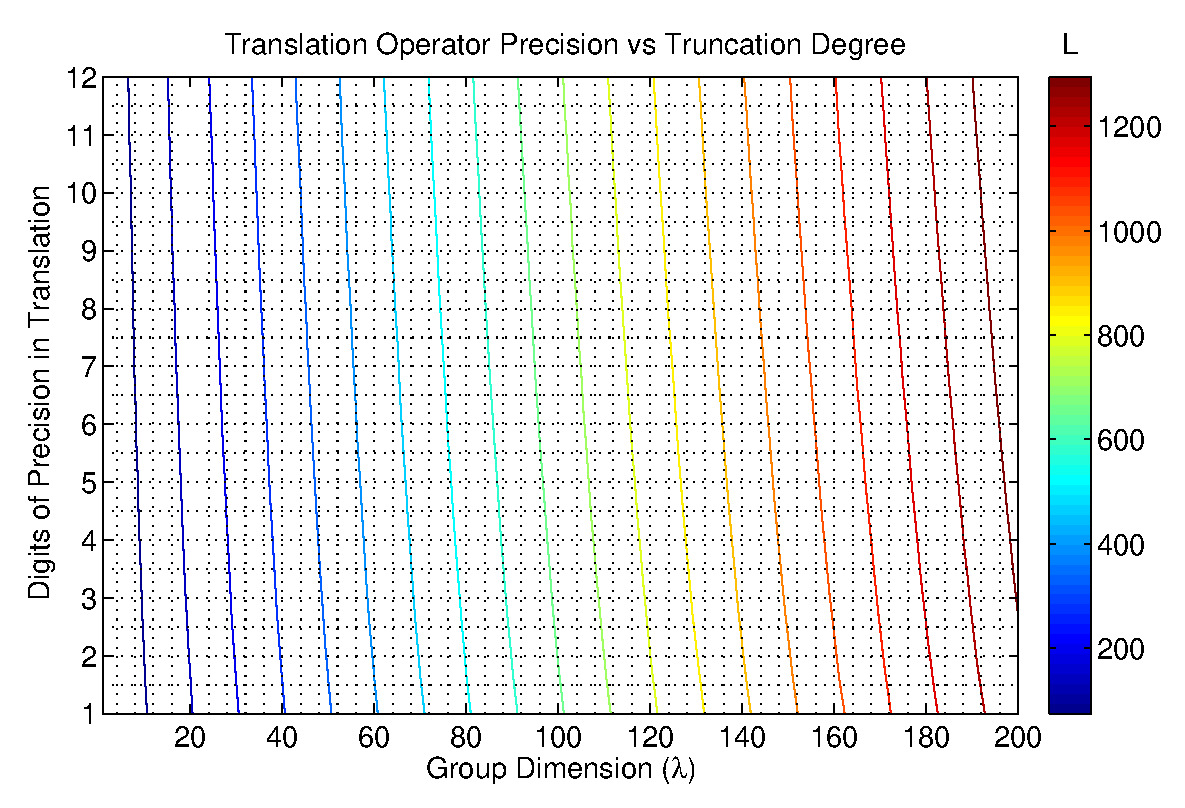
\includegraphics[width=3.5in]{FastMultipoleMethod/digvsL} 
%   \caption{}
%   \label{fig7}
%\end{figure}
%
% \begin{figure}[h] 
%   \centering
%   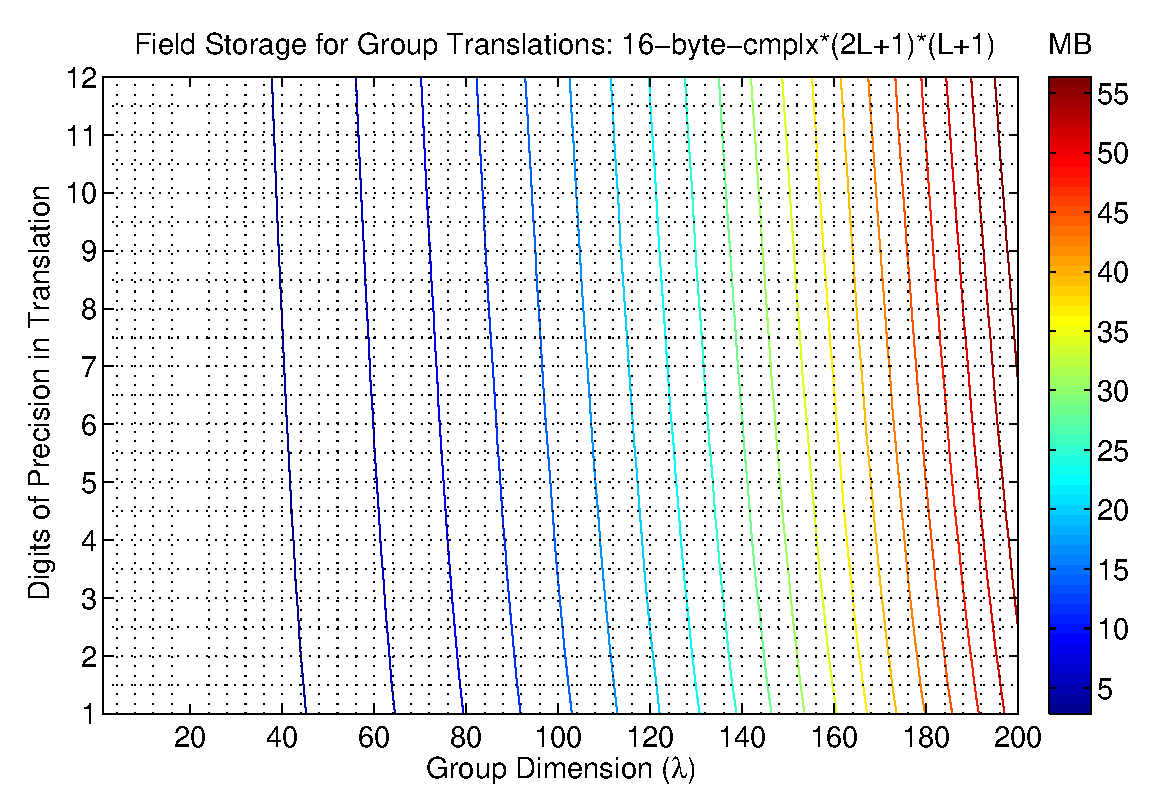
\includegraphics[width=3.5in]{FastMultipoleMethod/storgvsL} 
%   \caption{}
%   \label{fig8}
%\end{figure}
%
%\newpage
% 
%\section{FMM Structure}
%
%The box hierarchy is structured as regular octree with $N_{levs}$ levels.  The top is level 1, the lowest is $N_{levs}$.  The number of harmonics at each level, and thus the sampling, are determine by the dimension of the boxes at that level, the bandwidth formula, and the precision of translation between boxes at that level.  Interpolation and filtering operations do not depend on the location of the boxes, so the Legendre polynomials only have to be computed and stored per level transition and are good for the entire domain.  However, each unique translation matrix must be precomputed. 
%We require $L$ to be odd to have an even number of latitude points.  This ensures that latitudes points between levels do not coincide, which avoids the singularity in the core filter operation.  
%
%
%
%
%\subsection{Level Properties}
%
%The properties at each level are 
%
%\begin{table}[H]
%\caption{Properties of each level}
%\begin{center}
%\begin{tabular}{|c|c|}
%\hline
%Box edge dimension & $d$ \\
%\hline
%Maximum degree harmonic & $L$\\
%\hline
%Number of $\phi$ samples & $I = 2L + 1$ \\
%\hline
%Number $\theta$ samples & $J = L + 1$ \\
%\hline
%$\phi$ samples & $\phi_i = 2\pi i/I$, $i = 0,...,I-1$ \\
%\hline
%$\theta$ samples & $\theta_j = \arccos(\mu_j)$ \\
%\hline
%$J$ Gaussian quadrature nodes on $[-1,1]$ & $\mu_j$ \\
%\hline
%$J$ Gaussian quadrature weights & $w_j$ \\
%\hline
%\end{tabular}
%\end{center}
%\label{tab4}
%\end{table}%
%
%
%The routine \texttt{fmmL} computes the maximum degree harmonics and box dimensions at each level.  It takes the side length of the box at the top most level, the number of levels, and the precision of the translation and uses the extended bandwidth formula.  It  forces $L$ to be odd. 
%{\footnotesize
%\VerbatimInput{/Users/mshaynes/Desktop/Work/Database/fmmL.m}
%}
%
%The routine \texttt{fmmLevel} takes the harmonic degrees at each level computed in \texttt{fmmL} and computes the properties in Table \ref{tab4} for each level, stored in a structure array.  The nodes and weights of Gaussian quadrature are precomputed quickly and accurately to any degree $L$ using \texttt{legpts} from the package Chebfun.  
%
%
%{\footnotesize
%\VerbatimInput{/Users/mshaynes/Desktop/Work/Database/fmmLevel.m}
%}
%
%
%\subsection{Interpolation/Filter}
%
%There are $N_{levs}-1$ transitions that exist between $N_{levs}$ levels.  The sums in the interpolator or filter are limited by the maximum harmonic degree of the \textit{smaller} of the two levels.  Therefore, we index the transitions relative to the level that is being interpolated from, or filtered to.  Let the small of the two levels have maximum degree $L$, sampled in latitude at $\mu_j$, while the larger of the two levels has maximum degree $K$ sampled in latitude at $\mu_k$.  The only quantities that must be precomputed to compute a filter or interpolation between levels $l$ to $l+1$ are given in Table \ref{tab5}.  Once computed, the quantities in the table are good for any transition in the entire computational domain assuming the hierarchy of boxes is a regular octree.  
%
%
%\begin{table}[htbp]
%\caption{Precomputed quantities required to interpolate up from, or filter down to, level $l+1$.}
%\begin{center}
%\begin{tabular}{|c|c|c|}
%\hline
%Quantity & Interpolation & Filter \\
%\hline
%$\widetilde P_{L-1}^m (\mu_j)$ & \ & x \\
%\hline
%$\widetilde P_{L}^m (\mu_j)$ & x & x \\
%\hline
%$\widetilde P_{L+1}^m (\mu_j)$ & x & x  \\
%\hline
%$\widetilde P_{L-1}^m (\mu_k)$ & \ & x \\
%\hline
%$\widetilde P_{L}^m (\mu_k)$ & x & x \\
%\hline
%$\widetilde P_{L+1}^m (\mu_k)$ & x & \ \\
%\hline
%$\dfrac{d}{d\mu}\widetilde P_{L-1}^m (\mu_k)$, $\dfrac{d}{d\mu}\widetilde P_{L}^m (\mu_k)$& \ & x \\
%\hline
%1D FMM, $\mu_j$ source, $\mu_k$ observation & x & \ \\
%\hline
%1D FMM, $\mu_k$ source, $\mu_j$ observation & \ & x \\
%\hline
%\end{tabular}
%\end{center}
%\label{tab5}
%\end{table}
%
%Due to the nature of the sums in the filter or interpolation, all required Legendre polynomials only need to be computed for $m=-L,...,L$ on grids size $(2L+1)\times(L+1)$ or $(2L+1)\times(K+1)$.  For polynomials of degree $L-1$, values at $m=L$ are set to zero.  For polynomials of degree $L+1$, the sums that use these polynomials only reach $L$.  
%
%\subsubsection{Precomputed Structure Array}
%
%The routine \texttt{fmmIntFilt} returns a structure array containing the quantities in Table \ref{tab5} precomputed to interpolate or filter the far-field patterns between levels.  In Matlab, \texttt{fft} returns one-sided frequencies that correspond to harmonics $[0:M, -M:-1]$.  Our computation of Legendre polynomials returns the order $[-M:M]$.  We rearrange the polynomial harmonics to correspond to the FFT harmonics to avoid additional indexing. 
%
%{\footnotesize
%\VerbatimInput{/Users/mshaynes/Desktop/Work/Database/fmmIntFilt.m}
%}
%
%\subsubsection{Fast Interpolation/Filter for FMM}
%
%We provide two working versions of the fast vector interpolation and filter operations based on the two methods described above.  To summarize, method 1 relies on precomputed matrices for the core operation, is easier to implement, but is limited to $O(L^3)$ operations.  Method 2 uses the fast scalar filter at its core, requires correction terms, is more complicated, but can be accelerated with the 1D FMM to $O(L^2 log L)$ operations.  
%
%\subsubsection{Method 1}
%
%The routine \texttt{fmmvecinterp1} interpolates a vector field from level $l+1$ to $l$, while the routine and \texttt{fmmvecfilter1} filters a vector field from level $l$ to $l+1$.  They are designed to work with the precomputed matrices $A$ and $B$ stored in the structure array that is the output of \texttt{fmmIntFilt}.  The matrices are precomputed using the routine \texttt{fmmComputeInterpFilter}.
%
%{\footnotesize
%\VerbatimInput{/Users/mshaynes/Desktop/Work/Database/fmmvecinterp1.m}
%}
%
%{\footnotesize
%\VerbatimInput{/Users/mshaynes/Desktop/Work/Database/fmmvecfilter1.m}
%}
%
%{\footnotesize
%\VerbatimInput{/Users/mshaynes/Desktop/Work/Database/fmmComputeInterpFilter.m}
%}
%
%
%\subsubsection{Method 2}
%
%The routine \texttt{fmmvecinterp2} interpolates a vector field from level $l+1$ to $l$, while the routine and \texttt{fmmvecfilter2} filters a vector field from level $l$ to $l+1$.  They are designed to work with the precomputed quantities stored in the structure array that is the output of \texttt{fmmIntFilt}.  Each are implemented similarly as follows:
%
%\begin{enumerate}
%\item Application of the fast scalar interpolation from harmonic $L-1$ or fast scalar filter to harmonic $L-1$.  These are provided by the routines \texttt{fmminterpLm1} and \texttt{fmmfilterLm1}.  The field components are multiplied by $\sin\theta_j$ (interpolation) or $\sin\theta_k$ (filter) on input.   The routines assume that there is no singularity in the core operation (I.e., even number of latitude samples).  
%Two implementations of the core computation are available: straight matrix-vector multiplication of precomputed $1/(x_j-x-k)$ matrix, or 1D FMM.  At the moment, Matlab's matrix-vector multiplication is faster than our implementation of the 1D FMM.  This may change in a different language.  The 1D FMM version is commented but fully functional
%
%\item Direct computation of vector harmonic coefficients at $L$ and $L+1$.  This is done with \eqref{eqblm1} and \eqref{eqclm1}.  All multiplying factors in those equations are included during pre-computation in \texttt{fmmIntFilt}.
%
%\item Computation of the correction terms in equations \eqref{correct1}, \eqref{correct2}, \eqref{correct3}, \eqref{correct4} by the function \texttt{fmmCorrectionTerms}. 
%
%\item Computation of the scalar field corrections via \eqref{eqist1} and \eqref{eqist2}.  Factors of $2\pi$ that appear in the original filters have again been cancelled.  
%
%\item Sum the fields from the fast filter and corrected field to give the final filtered vector field components.  Divide the sum by $\sin\theta_j$.
%\end{enumerate}
%
%
%{\footnotesize
%\VerbatimInput{/Users/mshaynes/Desktop/Work/Database/fmmvecinterp2.m}
%}
%
%{\footnotesize
%\VerbatimInput{/Users/mshaynes/Desktop/Work/Database/fmminterpLm1.m}
%}
%
%{\footnotesize
%\VerbatimInput{/Users/mshaynes/Desktop/Work/Database/fmmvecfilter2.m}
%}
%
%{\footnotesize
%\VerbatimInput{/Users/mshaynes/Desktop/Work/Database/fmmfilterLm1.m}
%}
%
%{\footnotesize
%\VerbatimInput{/Users/mshaynes/Desktop/Work/Database/fmmCorrectionTerms.m}
%}
%
%\subsection{Octree}
%
%An octree is a recursive division of a cube into octants.  Each cube at a given level is called a group, which has at most 8 occupied children.  We use the publicly available Matlab routine \texttt{BuildOctree} to construct the octree.  It takes the $(x,y,z)$ coordinates of scatterer points and minimum group size.  It returns a structure array of group relations.  It prunes unoccupied groups and determines the near-neighbors.  We modify it in order to specific the edges of the bounding box (We will later replace the \texttt{neargrouptouch} array with the interlayer near neighbor list and add the interlayer interaction list.)  The routine \texttt{fmmInitializeTree} adds structure elements for $F_{\theta}$ and $F_{\phi}$ at each group.  
%
%%\begin{table}[htbp]
%%\caption{Properties of tree structure array}
%%\begin{center}
%%\begin{tabular}{|c|c|}
%%\hline
%%Level & $l$\\
%%\hline
%%Box index at this level & $i$ \\
%%\hline
%%Level of parent & $l+1$ \\
%%\hline
%%Global index of parent at level $l+1$  & $p$ \\
%%\hline
%%Octant in parent's box &  $1,...,8$ \\
%%\hline
%%Level of children & $l-1$ \\
%%\hline
%%Global indexes of children at level $l-1$ & $c_1$, $c_2$, ..., $c_n$ \\
%%\hline
%%Coordinates of box center & \bb{x} \\
%%\hline
%%Field components size $(2L+1)\times(L+1)$ & $F_{\theta}(\theta,\phi)$, $F_{\phi}(\theta,\phi)$  \\
%%\hline
%%\end{tabular}
%%\end{center}
%%\label{default}
%%\end{table}%
%
%
%\begin{table}[htbp]
%\caption{Properties of Tree structure array.}
%\begin{center}
%\begin{tabular}{|c|c|}
%\hline
%List of children per group per level & \texttt{Tree(l).group(g).child(c)} \\
%\hline
%Coordinates of group center & \texttt{Tree(l).group(g).groupcenter}  \\
%\hline
%Length of box edge & \texttt{Tree(l).group(g).cubelength}  \\
%\hline
%List of near-neighbors  & \texttt{Tree(l).group(g).neargrouptouch(nn)}  \\
%\hline
%$F_{\theta}(\theta,\phi)$, size $(2L+1)\times(L+1)$ & \texttt{Tree(l).group(g).Fth} \\
%\hline
%$F_{\phi}(\theta,\phi)$, size $(2L+1)\times(L+1)$  & \texttt{Tree(l).group(g).Fphi} \\
%\hline
%\end{tabular}
%\end{center}
%\label{default}
%\end{table}%
%
%
%{\footnotesize
%\VerbatimInput{/Users/mshaynes/Desktop/Work/Database/fmmInitializeTree.m}
%}
%
%
%
%
% \begin{figure}[htbp] 
%   \centering
%   \includegraphics[width=4in]{FastMultipoleMethod/octree} 
%   \caption{Octree structure of random points.  $N_{levs}$ = 5, maximum group size 10$\lambda$, minimum group size 0.625$\lambda$.}
%   \label{fig9}
%\end{figure}
%


%
%\subsection{Traditional Interaction List}
%
%The tradition FMM interaction list is constructed recursively starting at the top most level and sweeping the entire octree in order to build a near-neighbor list and interaction list for each group at each level.  The interaction list for a group consists of  groups that are in its so-called neighborhood, i.e., children of the near neighbors of its parent, that are not near neighbors to the group itself.  Neighborhood boxes are well removed, but the outgoing fields are not accounted for one level up because the parents are near neighbors.  [Adapted from Darve 2000]
%
%\begin{figure}[htbp]
%\begin{algorithmic}[1]
%\footnotesize
%\Function{Main}{}
%\State CurrentGroup = TopGroup
%\State Store CurrentGroup in NearNeighbor list of CurrentGroup
%\State \Call{BuildInteractionList}{CurrentGroup,Nlevs,level = 1}
%\EndFunction
%\\
%\Function{BuildInteractionList}{Parent,Nlevs,level}
%\If {level == Nlevs} \State {\Return} 
%\Else{  
%\For {Parent's NearNeighbors}
%\For{Neighborhood = Children of Parent's NearNeighbors}
%\For{Child = Children of Parent}
%\If {Neighborhood == Child's NearNeighbor}
%\State{Add Neighborhood to Child's NearNeighbor list}
%\Else
%\State{Add Neighborhood to Child's Interaction list}
%\EndIf
%\EndFor
%\EndFor
%\EndFor
%\For {Child = Children of Parent}
%\State \Call{BuildInteractionList}{Parent,Nlevs,level+1}
%\EndFor
%}
%\EndIf
%\EndFunction
%\end{algorithmic}
%\caption{Pseudocode for building a traditional FMM near-neighbor and interaction lists}\label{}
%\end{figure}
%
%
%\newpage
%
%\section{Multi-layer FMM Algorithm}
%
%The aim of the multi-layer FMM algorithm is to capture first-order scattering through dielectric layer interfaces in 3D domains that are many thousands of wavelengths.  The goal of the implementation is to capture enough of the relevant scattering physics while making the problem computationally tractable.  The scattering physics we need to capture are
%
%\begin{enumerate}
%\item Reflection, refraction, specularity, and rough surface effects at an interface.   
%\item First-order interactions between many facets between layers over Fresnel-zone sized regions.  
%\item Two-way propagation and reflection at each interface.
%\end{enumerate}
%
%Item 1 is accomplished with scattering matrices that capture scattering from facets that are used to discitize the interfaces.  Item 2 is accomplished via a user defined interaction rule in combination with FMM acceleration through aggregation/dissaggregation.  Item 3 is accomplished by sweeping the fields from the top interface to the bottom interface and back again.  On the return pass, upward transmission fields are combined with reflected fields from the same interface.  
%
%This algorithm drives two key elements: 1) a method of computation for scattering matrices of facets, 2) the construction of an different type of interaction list from the traditional one.  Scattering matrices transform all incoming plane waves into all outgoing plane waves, and, while large, fit naturally into the plane wave formulation of the FMM.  
%
%Diagrams
%
%
%
%
%\subsection{Multi-layer Interaction List}
%
%For a large multi-layer problem, we construct the interaction action list as follows: 
%
%\begin{enumerate}
%\item For scattering between layers, we only need a near-neighbor list and interaction list between layers, not within a layers.
%\item We only need to bookkeep near-neighbors and interactions from the interface of layer $n$ to $n+1$ (downward).  Reverse interactions are necessity captured in this list.  
%\item If there are $N$ interfaces, there are $N-1$ interaction lists.  
%\item For extremely large problems, we will likely not aggregate to the top most FMM level.  This is because the number of harmonics required is too large, or the storage for the groups will not be parallelizable.  We defined a maximum FMM level for translations.  When groups in two adjacent layers at the maximum level are well separated, the interaction list will be constructed with a rule we define (e.g., radiation cones).  When groups in two adjacent layers are neighbors (at the max level or below) the traditional interaction rules apply.  
%\item We will enforce the rule that the minimum spacing between two interfaces must greater than one box at the lowest FMM level, so that there are no near-neighbors at the lowest level.
%\end{enumerate}
%
%First define the points for each layer.  An FMM octree is constructed for the points of each layer.  Each layer octree is a subset of a global octree, such that boxes between layers are on the same global grid.  Next, create a layer structure array that contains the octree for all layers (in large problems, for example, this might be a link across files, one file per layer) and their dielectric properties.  Then, we identify groups at the max level in layer $n$ that have near neighbors in layer $n+1$ (including self terms) and construct the tradition interaction lists for them between the two layers.  
%
%
%\begin{figure}[hbtp]
%\begin{algorithmic}[1]
%\footnotesize
%\Function{Main}{}
%\For {layer = 1 to Nlayers}
%\State tree = \Call{BuildOctree}{layer}
%\State Add tree to Layer structure array
%\EndFor
%\State Initialize the trees in the Layer structure array with empty near neighbor and interaction lists that will point to groups indices in layer+1 (up to layer N-1)
%\For {layer = 1 to Nlayers-1}
%\For {CurrentGroup = Groups at max level}
%\State Find CurrentGroup near neighbors in layer+1 and if a self group.
%\EndFor
%\EndFor
%\For {layer =1 to Nlayers-1}
%\For {CurrentGroup = Groups at max level }
%\If {CurrentGroup has near neighbors in layer+1}
%\State \Call{BuildNNInteractionList}{CurrentGroup,layer,Nlevs,level = maxlevel}
%\EndIf
%\If {CurrentGroup has non-near neighbors in layer+1}
%\State \Call{BuildMaxLevelInteractionList}{CurrentGroup,layer,level = maxlevel}
%\EndIf
%\EndFor
%\EndFor
%\EndFunction
%\\
%\Function{BuildNNInteractionList}{Parent,layer,Nlevs,level}
%\If {level == Nlevs} \State {\Return} 
%\Else{  
%\For {Parent's NearNeighbors in layer+1}
%\For{Neighborhood = Children of Parent's NearNeighbors in layer+1}
%\For{Child = Children of Parent}
%\If {Neighborhood == Child's NearNeighbor in layer+1}
%\State{Add Neighborhood to Child's NearNeighbor list in layer+1}
%\Else
%\State{Add Neighborhood to Child's Interaction list in layer+1}
%\EndIf
%\EndFor
%\EndFor
%\EndFor
%\For {Child = Children of Parent}
%\State \Call{BuildNNInteractionList}{Child,layer,Nlevs,level+1}
%\EndFor
%}
%\EndIf
%\EndFunction
%\end{algorithmic}
%\caption{Pseudocode for building a multi-layer near-neighbor and interaction lists}\label{}
%\end{figure}
%
%% we have a maximum upper limit on level, due to size
%% the interactions at the max lev is decided by a different rule, (cone
%% size, interaction angle, parallelizable maximum level L < 600)
%% upper layer to lower, will capture all lower to upper as well
%% includes a self term
%% minimum spacing between layers determined so they are well separated at
%% the lowest level, because we have no direct/self terms.
%
%\newpage 
%
%The function \texttt{fmmLayerInteractionList} takes the layer structure array, maximum FMM level and returns the same structure array with near neighbor and interactions for $N-1$ layers.  It initializes the lists and finds the near neighbors at the maximum level.  It then calls \texttt{fmmInteractionList} which recursively down-traverses a group with any near-neighbors in the next level to form the lower level interaction lists.   The routine \texttt{fmmMaxLevelInteractionList} creates the interactions list between layers at the maximum level.  The rule here finds the groups at the maximum level in the next layer who's centers fall within a downward scattering cone.  
%
%{\footnotesize
%\VerbatimInput{/Users/mshaynes/Desktop/Work/Database/fmmLayerInteractionList.m}
%}
%
%{\footnotesize
%\VerbatimInput{/Users/mshaynes/Desktop/Work/Database/fmmNNInteractionList.m}
%}
%
%{\footnotesize
%\VerbatimInput{/Users/mshaynes/Desktop/Work/Database/fmmMaxLevelInteractionList.m}
%}
%
% \begin{figure}[htbp] 
%   \centering
%   \includegraphics[width=4in]{FastMultipoleMethod/layerNN} 
%   \caption{Near neighbors between a group in layer 1 and groups in layer 2.}
%   \label{fig10}
%\end{figure}
%
% \begin{figure}[htbp] 
%   \centering
%   \includegraphics[width=4in]{FastMultipoleMethod/layerInt} 
%   \caption{Interactions between a group in layer 1 groups in layer 2, who's parents are near neighbors but are themselves well separated.}
%   \label{fig1}
%\end{figure}
%
%
%
% \begin{figure}[htbp] 
%   \centering
%   \includegraphics[width=4in]{FastMultipoleMethod/cone} 
%   \caption{Interactions between a group in layer 1 those in layer 2 at the maximum level defined by a downward scattering cone.  Here the cone is has 30 degree half angle and pitch in the $-y$ direction of 12 degrees.}
%   \label{fig1}
%\end{figure}
%
%
%\newpage
%
%
%\subsection{Translation}
%
%The translation operators can be computed two ways: 1) precompute all unique translation operators for all interaction groups in their entirety and store them: 2) precompute the sampled translation operators and use the fast interpolated scheme before.  
%
%On a regular grid, the number of unique translations is greatly reduced.  At levels less than the maximum interaction level (not including the lowest level), a group has at most $3^3-1 = 26$ nearest neighbors, and at most $7^3-3^3-1 = 315$ possible interaction directions.  Given a maximum group level, when we transfer between layers, we may have many fewer or many more than 315 unique interactions.
%
%\begin{table}[htbp]
%\caption{Precomputed translation operators}
%\begin{center}
%\begin{tabular}{|c|c|}
%\hline
%Precomputed translation operators, for unique $kr$ & $T_L(\bb{k},\bb{X})$ \\
%\hline
%\end{tabular}
%\end{center}
%\label{default}
%\end{table}
%
%For this  Matlab implementation, we choose option 1) to precompute the unique translation operators in the forward and reverse directions and adds them to the layer structure.  We do this because the interpolation scheme is, at the moment, fairly slow.  This is done with the routine \texttt{fmmTranslationOperators}.  It finds the unique translations between interacting groups between each layer for each level and computed them.  It adds a list of interaction indices that index the translation operator for that group and the group in the next layer at the same position in the next-layer interaction list.  It then computes reverse interaction lists that point from a lower level to the next higher level.
%
%{\footnotesize
%\VerbatimInput{/Users/mshaynes/Desktop/Work/Database/fmmTranslationOperators.m}
%}
%
%
%\subsection{Layers Field Storage}
%
%Only outgoing fields from interacting groups must be stored. Incoming radiation patterns are computed during disaggregation on the fly.  An interface has one set of downward fields after transmission, and one set of upward fields after reflection and transmission from the lower layer on the return pass.  The fields are sampled on the usual $2L+1$ x $L+1$ phi/theta.  There are two exceptions: 1) at the top interface only transmitted fields are stored, 2) at the bottom interface only reflected fields are stored.  Reflection from the upper surface is computed separately between the source and the each facet directly, this will have benefits later.
%
%The routine \texttt{fmmInitializeLayerTree} creates this storage based on the interaction lists. 
%
%{\footnotesize
%\VerbatimInput{/Users/mshaynes/Desktop/Work/Database/fmmInitializeLayerTree.m}
%}
%
%\newpage 
%\subsection{Multi-layer Scattering Algorithm Psuedo-Code}
%
%\begin{figure}[htbp]
%\begin{algorithmic}[1]
%\footnotesize
%\State Create the layer interfaces (facet centers, facet normals, dielectric properties)
%\State Call \Call{BuildOctreeMod}{} to create FMM trees for each layer interface
%\State Create an $N\times1$ Layers struct array
%\State Add FMM layer interface trees to Layers struct
%\State Call \Call{fmmLayerInteractionList}{} to create the interaction lists and add them to Layers struct
%\State Call \Call{fmmLevel}{} to create level properties struct
%\State Call \Call{fmmIntFilt}{} to create interpolation and filter struct
%\State Call \Call{fmmTranslationOperators}{} to compute the unique translation operations in the interaction list and add them to the Layers struct
%\State Call \Call{fmmInitializeLayerTree}{} to create storage for all outgoing fields in Layers struct
%\State Compute $S_{11}$ for each facet directly to source \Comment{\textit{Surface return}}
%\For{Layer = top to bottom}\Comment{\textit{Downward pass}}
%\For{CurrentGroup = Groups at max level}
%%\State Copy tree struct for CurrentGroup, create temporary storage at each level.
%\If {Layer = top}
%\State Compute $S_{21}$ for each facet directly from source field
%\State Aggregate $S_{21}$ to max level and store as transmitted field
%\Else
%\State Translate and disaggregate incoming fields from layer above to facet level
%\State Compute $S_{11}$ for each facet
%\State Aggregate $S_{11}$ to max level and store as reflected field
%\If {Layer != bottom}
%\State Compute $S_{21}$ for each facet
%\State Aggregate $S_{21}$ to max level and store as transmitted field
%\EndIf
%\EndIf
%\EndFor{}
%\EndFor{}
%
%\For{Layer = next-to-last to top}\Comment{\textit{Upward pass}}
%\For{CurrentGroup = Groups at max level}
%\State Translate and disaggregate reflected fields from lower layer to facet level
%\If {Layer = top}
%\State Compute $S_{12}$ for each facet directly to source
%\State Compute $S_{11}$ for each facet directly to source 
%\State Sum $S_{12}$ and $S_{11}$ contributions to source received field
%\Else
%\State Compute $S_{12}$ for each facet
%\State Aggregate $S_{12}$ transmission to max level
%\State Add aggregated transmission to previously stored reflected fields
%\EndIf
%\EndFor{}
%\EndFor{}
%
%%\\
%%\\
%% \Function{Main}{}
%%\State CurrentGroup = TopGroup
%%\State Store CurrentGroup in NearNeighbor list of CurrentGroup
%%\State \Call{BuildInteractionList}{CurrentGroup,Nlevs,level = 1}
%%\EndFunction
%%\\
%%\Function{BuildInteractionList}{Parent,Nlevs,level}
%%\If {level == Nlevs} \State {\Return} 
%%\Else{  
%%\For {Parent's NearNeighbors}
%%\For{Neighborhood = Children of Parent's NearNeighbors}
%%\For{Child = Children of Parent}
%%\If {Neighborhood == Child's NearNeighbor}
%%\State{Add Neighborhood to Child's NearNeighbor list}
%%\Else
%%\State{Add Neighborhood to Child's Interaction list}
%%\EndIf
%%\EndFor
%%\EndFor
%%\EndFor
%%\For {Child = Children of Parent}
%%\State \Call{BuildInteractionList}{Parent,Nlevs,level+1}
%%\EndFor
%%}
%%\EndIf
%%\EndFunction
%\end{algorithmic}
%\caption{Pseudocode for the multi-layer FMM algorithm}\label{}
%\end{figure}
%
%\newpage 
%
%\subsection{Subtree Recursion Template}
%
%The routine \texttt{treeTraverse} is a template for recursing through a subtree given the starting level and group index.
%
%{\footnotesize
%\VerbatimInput{/Users/mshaynes/Desktop/Work/Database/treeTraverse.m}
%}
%
%\subsection{Create Subtree}
%
%Subtrees will be used to provide scratch space for aggregation and disaggregation of max level groups.  All max level groups that are well separated between layers only need to store the outgoing fields at the max level, not the underlying fields at each level of aggregation or disaggregation.  Therefore, we create scratch space in a subtree that contains field storage at every group.  We will transfer only the fields required for interacting groups to the global tree, then destroy the subtree.  This also makes aggregation/disaggregation easy, because we simply loop over all existing elements of the tree.  
%
%The routine \texttt{fmmMakeSubTree} will extract a subtree from the global tree for a given layer with a local parent/child indexing.   The subtree structure is initialized, then the routine calls \texttt{fmmTraverseNewTree} to determine the local parent/child indexing and group index in the global tree, and calls \texttt{fmmInitializeTree} to create field storage for every group in the subtree.  We give it another structure called \texttt{Pts}, which is a structure array containing the locations of the scatterers.  It will return a tree with storage down to the level of the scatterers.  
%
%
%{\footnotesize
%\VerbatimInput{/Users/mshaynes/Desktop/Work/Database/fmmMakeSubTree.m}
%}
%
%{\footnotesize
%\VerbatimInput{/Users/mshaynes/Desktop/Work/Database/fmmTraverseNewTree.m}
%}
%
%\subsection{Aggregate Subtree}
%
%The routine \texttt{fmmAggregateSubTree} will aggregate the fields up a subtree produced by \texttt{fmmMakeSubTree} starting at the scatterer level up to the max level.  The outgoing fields from the scatterers must first be loaded at the lowest level.  The wave number is a variable because will we aggregate the same tree in two different media (one for up going waves, one for down going waves).
%
%{\footnotesize
%\VerbatimInput{/Users/mshaynes/Desktop/Work/Database/fmmAggregateSubTree.m}
%}
%
%\subsection{Layer-to-layer Translation}
%
%Translations will be computed per group at the maximum level and loaded into the current subtree.  The direction of the translation, and therefore the operator and medium it was computed in will depend on the whether we are in the downward or upward pass of the layers.  
%
%The routine \texttt{fmmTranslateToSubTree} computes the translated fields to all level of the subtree that need it (i.e., nonzero interaction list).  It includes a flag (called 'add') to the subtree to indicate whether the disaggregation routine should add the the filtered field with the stored field or not.  
%
%{\footnotesize
%\VerbatimInput{/Users/mshaynes/Desktop/Work/Database/fmmTranslateToSubTree.m}
%}
%
%
%\subsection{Disaggregate Subtree}
%
%The routine \texttt{fmmDisaggregateSubTree} will disaggregate the fields in a subtree produced by \texttt{fmmMakeSubTree} starting at the maximum level down to the scatter level.  The incoming fields at all levels must be loaded.  Filtered fields are added to whatever existing fields already exist at that level based on the \texttt{add} switch.  The wave number is again a variable. 
%
%{\footnotesize
%\VerbatimInput{/Users/mshaynes/Desktop/Work/Database/fmmDisaggregateSubTree.m}
%}
%
%
%\subsection{Store Subtree}
%
%After a subtree as been aggregated to the max level, only the outgoing fields for groups with non-zero interaction lists need to be stored in the Layers structure.  
%
%The routine \texttt{fmmStoreSubTree} takes an aggregated subtree and identifies from the global indices which fields must be stored.  The string switch \texttt{TRstr} indicates if the fields are stored as reflected or transmitted fields.  The string switch \texttt{writestr} indicates whether to overwrite or add to existing fields.  
%
%{\footnotesize
%\VerbatimInput{/Users/mshaynes/Desktop/Work/Database/fmmStoreSubTree.m}
%}

\clearpage
\newpage

\section{Scattering Matrices for the FMM}

\subsection{S-matrix and Field Multiplication using Quadrature}

The scattering matrix (S-matrix) (or scattering function matrix, \cite{tsang2000scattering}) embeds the scattering behavior of an object as a mapping between incident and scattered plane waves of different incident and scattered directions and polarizations. In the FMM, fields are treated as expansions of plane waves where many plane waves are incident on a local region at once. The outgoing scattered field in any particular direction is the sum of scattering contributions from all incident waves. In the limit, this sum can be computed as an integral of incident directions over the unit sphere. Casting the  S-matrix this way allows it to be used in the structures of the FMM.  

For the FMM, we choose the orthonormal basis for the S-matrix formed by $\hat{k}$, $\hat{\theta}$, and $\hat{\phi}$, such that the incident and scattered fields are defined over two far-field patterns $\bb{F}(\theta_s,\phi_s)$ and $\bb{G}(\theta_i,\phi_i)$. \begin{equation}
\bb{E}_i(\hat{k}_i) = \left(G_{\theta}(\hat{k}_i)\hat{\theta}  +G_{\phi}(\hat{k}_i) \hat{\phi} \right) e^{i\bb{k}_i \cdot \br}
\end{equation}

\begin{equation}
\bb{E}_s(\hat{k}_s) = \left( F_{\theta}(\hat{k}_s)\hat{\theta} +  F_{\phi}(\hat{k}_s)\hat{\phi}\right) \dfrac{ e^{i k r}}{r}
\end{equation}
 
\begin{equation}
\twobyone{F_{\theta}(\hat{k}_s)}{F_{\phi}(\hat{k}_s)} = 
\twobytwo
{S_{\theta\theta}(\hat{k}_s,\hat{k}_i) }
{S_{\theta\phi}(\hat{k}_s,\hat{k}_i) }
{S_{\phi\theta}(\hat{k}_s,\hat{k}_i) }
{S_{\phi\phi}(\hat{k}_s,\hat{k}_i) }   
\twobyone{G_{\theta}(\hat{k}_i)}{G_{\phi}(\hat{k}_i)} 
\end{equation}

% Here, $\hat{\theta}$, and $\hat{\phi}$ are the same as the $\hat{h}$ and $\hat{v}$ polarizations in the 'wave-oriented' or 'forward scattering alignment' (FSA) polarization convention \cite{ulaby2014microwave}. %In addition, $\hat{\theta}$, and $\hat{\phi}$ are really the same polarization components relative to the frame of the scatterer, where $\hat{k}_i$ and $\hat{k}_s$ are just radial vectors in the direction of propagation. 
 
The matrix above maps any pair of direction/polarization to any other pair.  Define the operation that transforms an incoming field pattern, $\bb{G}(\hat{\bb{k}})$, to an outgoing field pattern, $\bb{F}(\hat{\bb{k}})$, as the integral of the S-matrix over the unit sphere of incident directions 
\begin{equation}
\bb{F}(\hat{\bb{k}}_s) = \int \overline{\bb{S}}(\hat{\bb{k}}_s,\hat{\bb{k}}_i)\cdot \bb{G}(\hat{\bb{k}}_i) d\Omega_{k_i}
\end{equation}

or
\begin{equation}
\twobyone{F_{\theta}(\hat{\bb{k}}_s)}{F_{\phi}(\hat{\bb{k}}_s)} = 
\int \twobytwo
{S_{\theta\theta}(\hat{\bb{k}}_s,\hat{\bb{k}}_i)}
{S_{\theta\phi}(\hat{\bb{k}}_s,\hat{\bb{k}}_i)}
{S_{\phi\theta}(\hat{\bb{k}}_s,\hat{\bb{k}}_i)}
{S_{\phi\phi}(\hat{\bb{k}}_s,\hat{\bb{k}}_i)}
\cdot \twobyone{G_{\theta}(\hat{\bb{k}}_i)}{G_{\phi}(\hat{\bb{k}}_i)} d\Omega_{k_i} \label{smatintegral}
\end{equation}

To compute this exactly, the field pattern and the S-matrix are sampled at the nodes of Gaussian quadrature on a grid that is $(2L+1) \times (L+1)$ for maximum harmonic degree $L$. Then \eqref{smatintegral} can be discretized as
 \begin{equation}
\twobyone{F_{\theta}(\theta_{\mu},\phi_{\nu})}{F_{\phi}(\theta_{\mu},\phi_{\nu})} = 
\dfrac{2\pi}{2L+1}  \sum_{i=1}^{2L+1} \sum_{j=1}^{L+1} w_j \twobytwo
{S_{\theta\theta}(\theta_{\mu},\phi_{\nu};\theta_j,\phi_i)}
{S_{\theta\phi}(\theta_{\mu},\phi_{\nu};\theta_j,\phi_i)}
{S_{\phi\theta}(\theta_{\mu},\phi_{\nu};\theta_j,\phi_i)}
{S_{\phi\phi}(\theta_{\mu},\phi_{\nu};\theta_j,\phi_i)} \cdot \twobyone{G_{\theta}(\theta_j,\phi_i)}{G_{\phi}(\theta_j,\phi_i)} 
\end{equation}

\noindent where the spherical angles $(\theta_j,\phi_i)$ and $(\theta_{\mu},\phi_{\nu})$ are the samples of quadrature.  Technically, only the incident directions needed to be sampled by quadrature. As always with quadrature, the poles are never sampled, so the polarization ambiguity at the poles never occurs. Writing this in matrix form, where the 2D spherical sum is over columns of the matrix, and the weights and multiplying constants are put in a diagonal matrix,\begin{equation}
\twobyone{\bb{F}_{\theta}}{\bb{F}_{\phi}} = 
\twobytwo{\overline{\bb{S}}_{\theta\theta}}{\overline{\bb{S}}_{\theta\phi}}{\overline{\bb{S}}_{\phi\theta}}{\overline{\bb{S}}_{\phi\phi}} \twobytwo{\bb{W}}{0}{0}{\bb{W}}\twobyone{\bb{G}_{\theta}}{\bb{G}_{\phi}}  \label{FSWG}
\end{equation}

\noindent where the elements of $\bb{W}$ contains copies of the weights $w_j$ as they apply to $\theta_j$.  

The routine \texttt{compute\char`_Smatrix\char`_quad} applies the S-matrix to an incoming field pattern when both are sampled on the points of Gaussian quadrature.  It returns the scattered field sampled the same way.  The fields are sized $I \times J$ where $I = 2L + 1$ and $J = L+1$ for maximum harmonic degree $L$ (as written the routine can take any sampling $I$ and $J$). The S-matrix block components are $I \times J \times I \times J$ with scattered directions in the first two dimensions and incident directions in the last two dimensions. The results match the same computation when its performed by starting with a S-matrix, converting it to a T-matrix, computing the scattering via harmonic expansions, and then converting it back to an S-matrix. 


{\footnotesize
\VerbatimInput{\code/FastMultipoleMethod/Smatrix/compute_Smatrix_quad.m}
}






%
%
%At a layer interface (e.g., surface facet), we can further define the scattering matrix with four components that account for two-way reflection and transmission at the interface such that
%
%
%\begin{equation}
%\twobyone{\bb{F}_1(\hat{\bb{k}}) }{\bb{F}_2(\hat{\bb{k}}) } = \twobytwo{\overline{\bb{S}}_{11} }{\overline{\bb{S}}_{12} }{\overline{\bb{S}}_{21} }{\overline{\bb{S}}_{22} }\twobyone{\bb{G}_1(\hat{\bb{k}}) }{\bb{G}_2(\hat{\bb{k}}) } 
%\end{equation}
%
%\noindent where $\bb{G}_1$ and $\bb{F}_1$ are incoming/outgoing fields in the upper region and $\bb{G}_2$ and $\bb{F}_2$ are in the lower region.  For facets, we can automatically enforce 'shadowing' by zeroing non-physical propagation combinations.  For example, $\overline{\bb{S}}_{11} $ should only transform downward incident plane waves into upward plane waves, relative to the facet normal, all other combinations are zero.  Likewise for the other components.  
%
%
% \begin{figure}[htbp] 
%   \centering
%   \includegraphics[width=3.5in]{FastMultipoleMethod/diagramsSmatrix} 
%   \caption{Components of a two-layer scattering matrix.}
%   \label{figxx}
%\end{figure}
%
%
% \begin{figure}[htbp] 
%   \centering
%   \includegraphics[width=5in]{FastMultipoleMethod/diagramsSmatrixk} 
%   \caption{Sampling scheme of plane wave directions or, equivalently, spherical angles. Incident directions are along columns, scattered directions are along rows.  Quadrants represent paris of $\pm k_{i,z}$ and $\pm k_{s,z}$.}
%   \label{figyy}
%\end{figure}
%
%
% \begin{figure}[htbp] 
%   \centering
%   \includegraphics[width=4in]{FastMultipoleMethod/diagramsSmatrix2} 
%   \caption{Coordinate and vector conventions for $S_{11}$ and $S_{21}$ in the FMM.}
%   \label{figyy}
%\end{figure}
%
%
% \begin{figure}[htbp] 
%   \centering
%   \includegraphics[width=4in]{FastMultipoleMethod/diagramsSmatrix3} 
%   \caption{Coordinate and vector conventions for $S_{12}$ and $S_{22}$ in the FMM.}
%   \label{figyy}
%\end{figure}
%


%
%\subsection{Scattering Matrix of a Kirchhoff Facet}
%
%We use the results of the Kirchhoff approximation to derive a scattering matrix for Kirchhoff facets in the context of the FMM.  Given an incident field 
%
%\[\bb{E}_i = \bb{e}_i E_o e^{i\bb{k}_i \cdot \bb{r}} \]
%
%the equations for the reflected and transmitted field from an entire facetized interface under the Kirchhoff approximation are
%
%\begin{eqnarray}
%\bb{E}_r(\br) & \approx & \dfrac{ik_1e^{ik_1r}}{4\pi r} E_o \left( \overline{\bb{I}} - \hat{k}_r \hat{k}_r \right)  \cdot \sum_n \bb{F}(\br_n) \int_{S_n} dS e^{i (\bb{k}_i - \bb{k}_r) \cdot \br}  \nonumber \\
%\bb{E}_t(\br) & \approx & -\dfrac{ik_2 e^{ik_2r}}{4\pi r} E_o \left( \overline{\bb{I}} - \hat{k}_t \hat{k}_t \right)  \cdot \sum_n \bb{N}(\br_n) \int_{S_n} dS  e^{i (\bb{k}_i - \bb{k}_t) \cdot \br}  \nonumber 
%\end{eqnarray}
%
%where
%
%\begin{eqnarray}
%\bb{F}(\br_n) &=&  - (\hat{e}_i \cdot \hat{q} )(\hat{n} \cdot \hat{k}_i) \hat{q} (1 - R^{\textrm{TE}}) \nonumber \\
%\ & \ & + (\hat{e}_i \cdot \hat{p} )(\hat{n} \times \hat{q}) (1 + R^{\textrm{TM}}) \nonumber \\
%\ & \ &+ (\hat{e}_i \cdot \hat{q} )(\hat{k}_r \times (\hat{n} \times \hat{q})) (1 + R^{\textrm{TE}}) \nonumber \\
%\ & \ & + (\hat{e}_i \cdot \hat{p} )(\hat{n} \cdot \hat{k}_i) (\hat{k}_r \times \hat{q}) (1 - R^{\textrm{TM}}) \\
%\bb{N}(\br_n) &=&  - \dfrac{\eta_2}{\eta_1}(\hat{e}_i \cdot \hat{q} )(\hat{n} \cdot \hat{k}_i) \hat{q} (1 - R^{\textrm{TE}})\nonumber \\
%\ & \ & + \dfrac{\eta_2}{\eta_1}(\hat{e}_i \cdot \hat{p} )(\hat{n} \times \hat{q}) (1 + R^{\textrm{TM}}) \nonumber \\
%\ & \ &+ (\hat{e}_i \cdot \hat{q} )(\hat{k}_t \times (\hat{n} \times \hat{q})) (1 + R^{\textrm{TE}}) \nonumber \\
%\ & \ & + (\hat{e}_i \cdot \hat{p} )(\hat{n} \cdot \hat{k}_i) (\hat{k}_t \times \hat{q}) (1 - R^{\textrm{TM}}) 
%\end{eqnarray}
%
%\noindent and $\bb{F}(\br')$ and $\bb{N}(\br')$ are treated constant over the surface of facets.  By definition, reflected directions $\hat{k}_r$ are in the upward direction above the facet in the first medium, while transmitted directions $\hat{k}_t$ are downward in the second medium.  
%
%To derive the scattering matrix of a single facet, we take one facet centered at the origin.  The surface sum reduces to  
%
%\begin{eqnarray}
%\bb{E}_r(\br) & \approx & \dfrac{ik_1 e^{ik_1 r}}{4\pi r} E_o \left( \overline{\bb{I}} - \hat{k}_r \hat{k}_r \right)  \cdot  \bb{F}(\hat{k}_i,\hat{k}_r) I(\bb{k}_i,\bb{k}_r)   \\
%\bb{E}_t(\br) & \approx & -\dfrac{ik_2e^{ik_2 r}}{4\pi r} E_o \left( \overline{\bb{I}} - \hat{k}_t \hat{k}_t \right)  \cdot  \bb{N}(\hat{k}_i,\hat{k}_t) I(\bb{k}_i,\bb{k}_t) 
%\end{eqnarray}
%
%\noindent where $\bb{F}(\hat{k}_i,\hat{k}_r)$ and $\bb{N}(\hat{k}_i,\hat{k}_t)$ depend on incident and scattered directions, surface normal, and material type.  The phase integral is one of
%
%\begin{eqnarray}
%I(\bb{k}_i,\bb{k}_r) &=&  \int_{S} dS  e^{i (\bb{k}_i - \bb{k}_r) \cdot \br}  \\
%I(\bb{k}_i,\bb{k}_t) &=&  \int_{S} dS  e^{i (\bb{k}_i - \bb{k}_t)\cdot \br }
%\end{eqnarray}
%
%Using they identity $ \overline{\bb{I}} - \hat{k} \hat{k} = \hat{\theta} \hat{\theta} + \hat{\phi} \hat{\phi}$ and separating the far-field phase and decay
%
%\begin{eqnarray}
%\bb{E}_r(\br) & \approx & \left( E_{\theta,s} \hat{\theta} + E_{\phi,s} \hat{\phi} \right)  \dfrac{e^{ik_1 r}}{r} \\
%\bb{E}_t(\br) & \approx & \left( E_{\theta,t} \hat{\theta} + E_{\phi,t} \hat{\phi} \right)  \dfrac{e^{ik_2 r}}{r} 
%\end{eqnarray}
%
%\begin{eqnarray}
%E_{\theta,s} &=& E_o\dfrac{ik_1 }{4\pi}\left(\hat{\theta}  \cdot  \bb{F}(\hat{k}_i,\hat{k}_r) \right)I(\bb{k}_i,\bb{k}_r) \\
%E_{\phi,s} &=& E_o\dfrac{ik_1 }{4\pi}\left(\hat{\phi}  \cdot  \bb{F}(\hat{k}_i,\hat{k}_r) \right)I(\bb{k}_i,\bb{k}_r) \\
%E_{\theta,t} &=& E_o\dfrac{ik_2 }{4\pi}\left(\hat{\theta}  \cdot  \bb{N}(\hat{k}_i,\hat{k}_t) \right)I(\bb{k}_i,\bb{k}_t) \\
%E_{\phi,t} &=& E_o\dfrac{ik_2 }{4\pi}\left(\hat{\phi}  \cdot  \bb{N}(\hat{k}_i,\hat{k}_t) \right)I(\bb{k}_i,\bb{k}_t) 
%\end{eqnarray}
%
%Noticing that $E_o$ is common with the incident field defined above, the vector components of the scattering matrix can be constructed by taking $\bb{e}_i = [\hat{\theta}, \hat{\phi}]$ in turn.
%
%For $S_{11}$ and $S_{21}$, the equations above are unchanged.  The incident directions come from above the facet, reflected waves propagate above the facet, and transmitted directions propagate below the facet.  For $S_{12}$ and $S_{22}$, we reverse the equations.  In both cases, the field components are projected onto the same local $\hat{q}$, $\hat{p}$ basis, so that the polarization transforms consistently between all four scattering matrices.  The reflection coefficients are determined by the local normal of the incident direction.  We zero incident/scattering angle combinations that are inconsistent with the definition each scattering matrix. 
%
%For the FMM, we can either derive a scattering matrix in the frame of the facet, requiring FMM fields to be rotated to the frame and back during computation, or we can create scattering matrices with the facet rotated in the global FMM frame. The later also fits more naturally into the structure of the FMM where plane wave directions are sampled and locked in the global frame, but ultimately it is a trade between computation and storage.  In either case, the FMM plane wave directions become reflected or transmitted depending on which side of the facet they originate. 
%
%
%
%
%\subsubsection{Kirchhoff Disk}
%
%The routine \texttt{sMatrixDisk} returns one of the four S-matrices for a Kirchhoff disk.  It takes as input the enumerated type ($S_{11}$, $S_{21}$, $S_{12}$, $S_{22}$), incident and scattering field directions, dielectrics and wave numbers of the upper and lower media, disk area and surface normal in the global FMM frame.  The reflection coefficients can be computed with complex $\epsilon_r$, but the phase integral will use the real part of the wave numbers for \texttt{intKirchhoffDisk}.  The incident and scattered directions are forced to 1D arrays, and using the $\theta$, $\phi$ grids defined in the FMM Level structure, will return wave vector directions consistent with the ordering in the figure above.  

%
%
%{\footnotesize
%\VerbatimInput{/Users/mshaynes/Desktop/Work/Database/sMatrixDisk.m}
%}
%
%
%
%
% \begin{figure}[htbp] 
%   \centering
%   \includegraphics[width=4in]{FastMultipoleMethod/S_{11}Disk} 
%   \caption{$S_{11}$ for disk $\hat{n} = [0,0,1]$, $a = 1/4 \lambda$, $\epsilon_{r1} = 1$, $\epsilon_{r2} = 3$}
%   \label{figyy}
%\end{figure}
%
% \begin{figure}[htbp] 
%   \centering
%   \includegraphics[width=4in]{FastMultipoleMethod/S_{21}Disk} 
%   \caption{$S_{21}$ for disk $\hat{n} = [0,0,1]$, $a = 1/4 \lambda$,$\epsilon_{r1} = 1$, $\epsilon_{r2} = 3$.  The fading stripe in the amplitude is due to the Brewster angle.  }
%   \label{figyy}
%\end{figure}
%
% \begin{figure}[htbp] 
%   \centering
%   \includegraphics[width=4in]{FastMultipoleMethod/S_{12}Disk} 
%   \caption{$S_{12}$ for disk $\hat{n} = [0,0,1]$, $a = 1/4 \lambda$,$\epsilon_{r1} = 1$, $\epsilon_{r2} = 3$}
%   \label{figyy}
%\end{figure}
%
% \begin{figure}[htbp] 
%   \centering
%   \includegraphics[width=4in]{FastMultipoleMethod/S_{22}Disk} 
%   \caption{$S_{22}$ for disk $\hat{n} = [0,0,1]$, $a = 1/4 \lambda$,$\epsilon_{r1} = 1$, $\epsilon_{r2} = 3$.  The fading patterns are due to the partial effects of total internal reflection (not complete total internal reflection because the disk the finite)}
%   \label{figyy}
%\end{figure}
%
%%% 
%
% \begin{figure}[htbp] 
%   \centering
%   \includegraphics[width=4in]{FastMultipoleMethod/S_{11}Disk2} 
%   \caption{$S_{11}$ for disk $\hat{n} = [0,1/\sqrt{2},1/\sqrt{2}]$, $a = 1/4 \lambda$, $\epsilon_{r1} = 1$, $\epsilon_{r2} = 3$}
%   \label{figyy}
%\end{figure}
%
% \begin{figure}[htbp] 
%   \centering
%   \includegraphics[width=4in]{FastMultipoleMethod/S_{21}Disk2} 
%   \caption{$S_{21}$ for disk $\hat{n} = [0,1/\sqrt{2},1/\sqrt{2}]$, $a = 1/4 \lambda$, $\epsilon_{r1} = 1$, $\epsilon_{r2} = 3$}
%   \label{figyy}
%\end{figure}
%
% \begin{figure}[htbp] 
%   \centering
%   \includegraphics[width=4in]{FastMultipoleMethod/S_{12}Disk2} 
%   \caption{$S_{12}$ for disk $\hat{n} = [0,1/\sqrt{2},1/\sqrt{2}]$, $a = 1/4 \lambda$, $\epsilon_{r1} = 1$, $\epsilon_{r2} = 3$}
%   \label{figyy}
%\end{figure}
%
% \begin{figure}[htbp] 
%   \centering
%   \includegraphics[width=4in]{FastMultipoleMethod/S_{22}Disk2} 
%   \caption{$S_{22}$ for disk $\hat{n} = [0,1/\sqrt{2},1/\sqrt{2}]$, $a = 1/4 \lambda$, $\epsilon_{r1} = 1$, $\epsilon_{r2} = 3$}
%   \label{figyy}
%\end{figure}



\subsection{S-matrix to T-matrix Transformation using Quadrature}
\label{fastStoT}

While the S-matrix is a useful 4D structure for storing the scattering properties of a target, it 1) can be difficult and inaccurate to interpolate if the propagation directions are not highly oversampled, and 2) it can be difficult to rotate between two reference frames because the wave directions and the vector components need to be transformed. On the other hand, the transition matrix (T-matrix), which relates coefficients of the incident and scattered spherical harmonic expansions, is very easy to rotate, and enables exact interpolation at arbitrary propagation directions through field expansions.  

Recall the S-matrix to T-matrix transformation \eqref{StoTBC}
\eq{\tbt{\overline{\bb{T}}^{MM}}{\overline{\bb{T}}^{MN} }{\overline{\bb{T}}^{NM}}{\overline{\bb{T}}^{NN}}  
=
\dfrac{k}{4\pi} 
\twobytwo{\overline{\bb{L}}_1^{-1}}{0}{0}{\overline{\bb{L}}_2^{-1}} 
\twobytwo{\overline{\bb{C}}_{\theta}^*}{\overline{\bb{C}}_{\phi}^*}{\overline{\bb{B}}_{\theta}^* } {\overline{\bb{B}}_{\phi}^*} 
\twobytwo{\bb{W}}{0}{0}{\bb{W}} 
\twobytwo
{\overline{\bb{S}}_{\theta\theta} }
{\overline{\bb{S}}_{\theta\phi}}
{\overline{\bb{S}}_{\phi\theta} }
{\overline{\bb{S}}_{\phi\phi} }   
\twobytwo{\bb{W}}{0}{0}{\bb{W}} 
\twobytwo{\overline{\bb{C}}_{\theta}}{\overline{\bb{B}}_{\theta}}{\overline{\bb{C}}_{\phi}}{\overline{\bb{B}}_{\phi}} 
\twobytwo{\overline{\bb{L}}_2}{0}{0}{\overline{\bb{L}}_1} \label{StoTvst}}

Our routine \texttt{vst} will compute exactly the discretized integral of the vector spherical harmonics over the unit sphere when applied from the left to the columns of $\bb{S}$, when the scattered directions $\bb{S}$ are sampled at the nodes of Gaussian quadrature. It can also be used again to compute the integral over incident directions as a left operation on $\bb{S}^*$.

The routine \texttt{convert\char`_S\char`_to\char`_T} computes the S-matrix to T-matrix transformation \eqref{StoTvst}. It takes as input the four S-matrix components and returns the four components of the T-matrix. Each S-matrix component is stored on a 4D grid that is $I \times J \times I \times J$, where $I = 2L+1$ and $J = L+1$ are sampled according to quadrature for $L$ harmonics. The scattered directions are dimensions 1 and 2 and the incident directions are dimensions 3 and 4. The routine returns the four components of the T-matrix up to harmonic degree $L$ all $m$ linearly indexed, each an $N \times N$ matrix where $N = L^2 + 2L$. The routine calls \texttt{vst} with precomputed Legendre polynomials and carries out the block matrix multiplication as a sequence of operations on the columns of the S-matrix or its transpose. The columns of the S-matrix are in fact the $I \times J$ subfields that are converted to columns of the T-matrix that are pairs of coefficients length $N$. This uses the fully normalized vector spherical harmonics.
\clearpage

{\footnotesize
\VerbatimInput{\code/FastMultipoleMethod/Smatrix/convert_S_to_T.m}
}



\subsection{T-matrix to S-matrix Transformation using Quadrature}
\label{fastTtoS}

Recall the T-matrix to S-matrix transformation \eqref{TtoSBC}
\eq{\twobytwo
{\overline{\bb{S}}_{\theta\theta} }
{\overline{\bb{S}}_{\theta\phi}}
{\overline{\bb{S}}_{\phi\theta} }
{\overline{\bb{S}}_{\phi\phi} }   
=
\dfrac{4\pi}{k} \twobytwo{\overline{\bb{C}}_{\theta}}{\overline{\bb{B}}_{\theta}}{\overline{\bb{C}}_{\phi}}{\overline{\bb{B}}_{\phi}}\twobytwo{\overline{\bb{L}}_1}{0}{0}{\overline{\bb{L}}_2} \tbt{\overline{\bb{T}}^{MM}}{\overline{\bb{T}}^{MN} }{\overline{\bb{T}}^{NM}}{\overline{\bb{T}}^{NN}}  \twobytwo{\overline{\bb{L}}_2^{-1}}{0}{0}{\overline{\bb{L}}_1^{-1}} \twobytwo{\overline{\bb{C}}_{\theta}^*}{\overline{\bb{C}}_{\phi}^*}{\overline{\bb{B}}_{\theta}^* } {\overline{\bb{B}}_{\phi}^*} \label{Sivst}} 

Our routine \texttt{ivst} will compute exactly the matrix multiplication over the block vector spherical harmonics when applied as a left operation to the columns of the T-matrix. We can use it again to compute the right multiplication of the conjugate operation as a left multiplication of the conjugate T-matrix, $\bb{T}^*$.

The routine \texttt{convert\char`_T\char`_to\char`_S}, computes the four components of the S-matrix given the four components of the T-matrix that contain harmonics up to degree $L$ all $m$ linearly indexed. It calls \texttt{ivst} to compute \eqref{Sivst} as a sequence of operations over the columns of the T-matrix or its transpose. The columns of the T-matrix are treated as pairs of expansion coefficients having $N = L^2 + 2L$ harmonics each when input to \texttt{ivst} that return field quantities sized $I \times J$ that are the new columns. When done, the S-matrix is $I \times J \times I \times J$ with scattered directions in the first two dimensions and incident directions in the last two dimensions.  Applied in sequence with \texttt{convert\char`_S\char`_to\char`_T} the routines will return identical results. Note, these two transformations do not require physically realistic T- or S-matrices, but an unrealistic S-matrix will be filtered into a band-limited T-matrix.   %Use string switch \texttt{'norm'} to transform from the normalized T-matrix.  

{\footnotesize
\VerbatimInput{\code/FastMultipoleMethod/Smatrix/convert_T_to_S.m}
}



%
%\newpage 
%
%\section{FMM Formulation}
%
%The dyadic Green's function is give by
%
%\begin{equation}
% \overline{\bb{G}}(\br,\br') = \left[\overline{\bb{I}} + \dfrac{1}{k^2} \nabla\nabla \right] g(\br,\br') 
% \end{equation}
% 
% where 
% 
% \[ g(\br,\br') =  \dfrac{e^{ik\vert \br - \br' \vert}}{4\pi \vert \br - \br' \vert} \]
%
%The far-field dyadic Green's function is 
%
%\begin{equation}
% \overline{\bb{G}}_f(\br,\br') \approx \left[\overline{\bb{I}} - \hat{\bb{k}} \hat{\bb{k}} \right] g(\br,\br') 
% \end{equation}
%
%
%The curl of the far expression can be derived as
%
%\[ \nabla \times \overline{\bb{G}}_f(\br,\br')  = \nabla \times \left( \left[\overline{\bb{I}} - \hat{\bb{k}} \hat{\bb{k}} \right] g(\br,\br')\right) \]
%
%This has the form
%
%\[ \nabla \times ( \phi \overline{\bb{F}} ) = \nabla \phi \times \overline{\bb{F}} + \phi \nabla \times \overline{\bb{F}} \]
%
%where $ \overline{\bb{F}}  = \overline{\bb{I}} - \hat{\bb{k}} \hat{\bb{k}}  $. This reduces to 
%
%\[ \nabla \times \overline{\bb{G}}_f(\br,\br')  = \nabla g(\br,\br') \times \left[\overline{\bb{I}} - \hat{\bb{k}} \hat{\bb{k}} \right]  \]
%
%Applied to a vector $\bb{v}$, 
%
%\begin{eqnarray}
%\left( \nabla \times \overline{\bb{G}}_f(\br,\br')\right)  \cdot \bb{v} & = &  -\bb{v} \cdot \left( \nabla \times \overline{\bb{G}}_f(\br,\br')\right) \\
%\ & = &  - \bb{v} \cdot  \left(\nabla g(\br,\br') \times \left[\overline{\bb{I}} - \hat{\bb{k}} \hat{\bb{k}} \right] \right) \\
% \ & = & - \left( \bb{v} \times \nabla g(\br,\br') \right) \cdot \left[\overline{\bb{I}} - \hat{\bb{k}} \hat{\bb{k}} \right] \\
% \ & = & -\left[\overline{\bb{I}} - \hat{\bb{k}} \hat{\bb{k}} \right] \cdot \left( \bb{v} \times \nabla g(\br,\br') \right) \\
% \ & = &  \left[\overline{\bb{I}} - \hat{\bb{k}} \hat{\bb{k}} \right] \cdot \left( \nabla g(\br,\br') \times \bb{v}  \right) \\
%  \ & \approx &  \left[\overline{\bb{I}} - \hat{\bb{k}} \hat{\bb{k}} \right] \cdot \left( i k g(\br,\br')\right) \left( \hat{\bb{k}} \times \bb{v} \right) 
% \end{eqnarray}
%
%The first equation because the curl of the dyadic Green's function is anti-symmetric.  The third equation uses the relation $\bb{a}\cdot(\bb{b} \times \overline{\bb{c}}) = (\bb{a} \times \bb{b})\cdot  \overline{\bb{c}} $.  The fourth  because $ \left[\overline{\bb{I}} - \hat{\bb{k}} \hat{\bb{k}} \right] $ is a symmetric dyad.  The fifth equation is cross product commutation.  Finally the gradient is applied and the far-field taken since 
%
%\[\nabla g(\br,\br')  = \left(ik - \dfrac{1}{r}\right) g(\br,\br') \hat{\bb{k}} \]
%
%\subsection{Spectral Representation}
%
%The spectral representation of the exponent is 
%
%\[ \dfrac{e^{ik\vert \br - \br' \vert}}{\vert \br - \br' \vert}  \approx \dfrac{ik}{4\pi} \int e^{i\bb{k}\cdot(\br - \br_o)} T_L(\bb{k},\bb{X}) e^{i\bb{k}\cdot(\br' - \br_s) }d\Omega \]
%
%The far field scalar Green's function is then
%
% \[ g(\br,\br') \approx \dfrac{ik}{16\pi^2} \int e^{i\bb{k}\cdot(\br - \br_o)} T_L(\bb{k},\bb{X}) e^{i\bb{k}\cdot(\br' - \br_s) }d\Omega \]
%
%And the dyadic Green's function is
%
%
%\begin{equation}
% \overline{\bb{G}}_f(\br,\br') \approx \dfrac{ik}{16\pi^2} \int  \left[\overline{\bb{I}} - \hat{\bb{k}} \hat{\bb{k}} \right]  e^{i\bb{k}\cdot(\br - \br_o)} T_L(\bb{k},\bb{X}) e^{i\bb{k}\cdot(\br' - \br_s) }d\Omega 
% \end{equation}
%
%\subsubsection{Source Volume Integral}
%
%The electric field due to a source is 
%
%\[ \bb{E}(\br) = i \omega \mu \int \overline{\bb{G}}_f(\br,\br') \cdot \bb{J}(\br') dV \]
%
%Substituting the dyadic Green's function we can write this
%
%\[ \bb{E}(\br) =  \dfrac{i k}{4 \pi}  \int \bb{F}(\hat{\bb{k}})  e^{i\bb{k}\cdot(\br - \br_o)} T_L(\bb{k},\bb{X}) d\Omega  \]
%
%where
%
%\[\bb{F}(\hat{\bb{k}}) =  \dfrac{1}{4 \pi}  (i \omega \mu) \left[\overline{\bb{I}} - \hat{\bb{k}} \hat{\bb{k}} \right] \cdot \int  e^{i\bb{k}\cdot(\br' - \br_s) }\bb{J}(\br') dV \]
%
%where $\bb{F}(\hat{\bb{k}}) $ is the far pattern of the source.
%
%\subsubsection{Surface Integrals}
%
%The reflected and transmitted fields above and below the boundary, respectively, are given by
%
%\begin{eqnarray}
%\bb{E}_r(\br) & = & \int_S dS' \left\{ i\omega \mu \G{1} \cdot \hat{n}' \times \bb{H}(\br') + \left[\nabla \times \G{1} \right] \cdot \hat{n}' \times \bb{E}(\br')\right\} \nonumber \\
%\bb{E}_t(\br) & = & \int_S dS' \left\{ i\omega \mu \G{2} \cdot \hat{n}_d' \times \bb{H}(\br') + \left[\nabla \times \G{2} \right] \cdot \hat{n}_d' \times \bb{E}(\br')\right\}  \nonumber
%\end{eqnarray}
%
%where $\hat{n}$ and $\hat{n}_d$ are the outward and inward pointing surface normals, and $\bb{E}$ and $\bb{H}$ are the fields on the boundary.
%
%Generically, these are 
%
%\begin{eqnarray}
%\bb{E}(\br) & = & \int_S dS' \left\{ i\omega \mu \G{} \cdot \hat{n}' \times \bb{H}(\br') + \left[\nabla \times \G{} \right] \cdot \hat{n}' \times \bb{E}(\br')\right\} \nonumber \\
%\end{eqnarray}
%
%Substituting the far field dyadic Green's function 
%
%\begin{eqnarray}
%\bb{E}(\br) & = & \int_S dS' \left\{ i\omega \mu \left[\overline{\bb{I}} - \hat{\bb{k}} \hat{\bb{k}} \right] g(\br,\br')  \cdot \hat{n}' \times \bb{H}(\br') \right. \nonumber \\
%\ & \ & \left. + \left[\overline{\bb{I}} - \hat{\bb{k}} \hat{\bb{k}} \right] \cdot \left( i k g(\br,\br')\right) \left(  \hat{\bb{k}} \times \left( \hat{n}' \times \bb{E}(\br')\right)\right) \right\} \nonumber 
%\end{eqnarray}
%
%which is
%
%\begin{eqnarray}
%\bb{E}(\br) & = & \int_S dS' \left[\overline{\bb{I}} - \hat{\bb{k}} \hat{\bb{k}} \right] \cdot  \left( i\omega \mu \left(\hat{n}' \times \bb{H}(\br')\right) +  i k  \hat{\bb{k}} \times \left( \hat{n}' \times \bb{E}(\br')\right)   \right) g(\br,\br')  \nonumber 
%\end{eqnarray}
%
%As before, substitute the spectral representation of the scalar Green's function, we can write fields as
%
%\[ \bb{E}(\br) =  \dfrac{i k}{4 \pi} \int \bb{F}(\hat{\bb{k}})  e^{i\bb{k}\cdot(\br - \br_o)} T_L(\bb{k},\bb{X}) d\Omega  \]
%
%\[\bb{F}(\hat{\bb{k}}) =  \dfrac{1}{4 \pi} \int \left[\overline{\bb{I}} - \hat{\bb{k}} \hat{\bb{k}} \right] \cdot   \left( i\omega \mu \left(\hat{n}' \times \bb{H}(\br')\right) +  i k  \hat{\bb{k}} \times \left( \hat{n}' \times \bb{E}(\br')\right)   \right)  e^{i\bb{k}\cdot(\br' - \br_s) } dS' \]
%
%Next assume the incident field has the form 
%
%\[ \bb{E}_{inc}(\br) =  \dfrac{i k}{4 \pi} \int \bb{F}_{inc} (\hat{\bb{k}}')  e^{i\bb{k}'\cdot(\br - \br_o)} T_L(\bb{k}',\bb{X}) d\Omega'  \]
%
%For plane waves, the magnetic field is
%
%\[ \bb{H}_{inc}(\br) = \dfrac{1}{\eta} \hat{\bb{k}} \times \bb{E}_{inc}(\br) \]
%
%The goal is the write $\bb{F}(\hat{\bb{k}})$ as 
%
%\[ \bb{F}(\hat{\bb{k}}) = \int \overline{\bb{S}}(\hat{\bb{k}},\hat{\bb{k}}') \cdot  \bb{F}_{inc} (\hat{\bb{k}}') T_L(\bb{k}',\bb{X}) d\Omega' \]
%
%where $\overline{\bb{S}}(\hat{\bb{k}},\hat{\bb{k}}')$ is the scattering matrix.  
%
%
%%
%%\section{Dyadic Green's Function Representations}
%%
%%\subsection{Forms of the Dyadic Green's Function}
%%
%%\subsubsection{Form 1}
%%
%%The explicit expression for the dyadic Green's function is given by
%%
%%\begin{equation}
%% \overline{\bb{G}}(\br,\br') = \left[\overline{\bb{I}} + \dfrac{1}{k^2} \nabla\nabla \right] \dfrac{e^{ik\vert \br - \br' \vert}}{4\pi \vert \br - \br' \vert}
%% \end{equation}
%%
%%See Chapter 1 for details.
%%
%%\subsubsection{Form 2}
%%
%%The dyadic Green's function written as an expansion of vector wave functions is
%%
%%\begin{equation}
%%\overline{\mathbf{G}}(\br,\br') = 
%%ik\displaystyle\sum\limits_{lm} \dfrac{1}{l(l+1)}\left[\M{\br}\Re\Mhat{\br'}  +  \N{\br}\Re\Nhat{\br'}\right] 
%%\end{equation}
%%
%%for $\vert \br' \vert < \vert \br \vert $.
%%
%%
%%
%%\subsubsection{Form 3}
%%
%%The far-field approximation of the dyadic Green's function used in the FMM is given by
%%
%%\begin{equation}
%%\overline{\mathbf{G}}(\br,\br') \approx \dfrac{ik}{4\pi} \int_S \left(\overline{\bb{I}} - \hat{\bb{k}}\hat{\bb{k}}'\right) 
%%e^{i \bb{k}\cdot(\bb{r}-\bb{r}_o) } T_L(\bb{k},\bb{X}) e^{-i \bb{k}\cdot(\bb{r}'-\bb{r}_s) } d^2\hat{\bb{k}}
%%\end{equation}
%%
%%where 
%%
%%\begin{eqnarray}
%%\bb{r} &=& \textrm{Observation point} \nonumber \\
%%\bb{r}_o &=& \textrm{Observation frame origin} \nonumber \\
%%\bb{r}' &=& \textrm{Source point} \nonumber \\
%%\bb{r}_s &=& \textrm{Source frame origin} \nonumber \\
%%\bb{X} = \bb{r}_o - \bb{r}_s &=& \textrm{Vector between origins} \nonumber \\
%%\bb{k} = k \hat{\bb{k}}  &=& \textrm{Wave vectors of the expansion} \nonumber \\
%%\hat{\bb{k}} &=& \textrm{Plane wave directions on the unit sphere}\nonumber
%%\end{eqnarray}
%%
%%
%%\subsection{Equivalency}
%%
%%We want to show the equivalent between all three forms of the dyadic Green's function.  This is to validate the computation of $T_L(\bb{k},\bb{X})$.  The electric field radiated from a current density $\bb{J}(\bb{r})$ is given by
%%
%%\begin{equation}
%%\bb{E}(\br) = i\omega\mu\int \overline{\bb{G}}(\br,\br')\cdot \bb{J}(\bb{r}) dV'
%%\end{equation}
%%
%%Let the current density be a Hertzian dipole at the origin
%%
%%\[ \bb{J}(\bb{r})  = I \hat{z} \delta(\br) \]
%%
%%\subsubsection{Form 1}
%%
%%Substituting the current density above into the integral above and using the Cartesian form of the dyadic Green's function the electric field everywhere is
%%
%%\begin{eqnarray}
%%\bb{E}(\br) &=& i\omega\mu\int \overline{\bb{G}}(\br,\br')\cdot I \hat{z} \delta(\br') dV' \\
%%\ &=& i\omega\mu I \thrcol{G_{xz}(\br,0) }{G_{yz}(\br,0) }{G_{zz}(\br,0)}
%%\end{eqnarray}
%%
%%\subsubsection{Form 2}
%%
%%\begin{eqnarray}
%%\bb{E}(\br) &=& i\omega\mu\int \overline{\bb{G}}(\br,\br')\cdot I \hat{z} \delta(\br') dV' \\
%%\ &=& i\omega\mu \int ik\displaystyle\sum\limits_{lm} \dfrac{1}{l(l+1)}\left[\M{\br}\Re\Mhat{\br'}  +  \N{\br}\Re\Nhat{\br'}\right] \cdot I \hat{z} \delta(\br') dV' \\
%%\ &=& \displaystyle\sum\limits_{lm} a_{lm} \M{\br}  + b_{lm} \N{\br}
%%\end{eqnarray}
%%
%%where
%%
%%\begin{eqnarray}
%%a_{lm} &=& \dfrac{1}{l(l+1)}i\omega\mu (ik) I \Re\Mhat{0}  \cdot \hat{z} \\
%%b_{lm} &=& \dfrac{1}{l(l+1)}i\omega\mu (ik) I \Re\Nhat{0}  \cdot \hat{z}
%%\end{eqnarray}
%%
%%The $z$ unit vector can be written $\hat{z} = \cos\theta \hat{r} - \sin\theta \hat{\theta}$.  
%%
%%The Bessel function expressions in the regular wave functions have the following limits at the origin
%%
%%\begin{eqnarray}
%%j_l(kr) &=& 0, \quad l \ge 1 \\ 
%%j_l(kr)/kr  &=& 1/3, \quad l = 1 , \quad 0, \quad \textrm{o.w.}\\
%%\dfrac{[krj_l(kr)]'}{kr} &=& 2/3, \quad l = 1, \quad 0, \quad \textrm{o.w.}
%%\end{eqnarray}
%%
%%
%%
%%
%%\begin{eqnarray}
%%a_{lm} &=& 0 \\
%%b_{lm} &=& i\omega\mu (ik) I \Re\Nhat{0}  \cdot \hat{z}
%%\end{eqnarray}
%%
%%
%%\subsubsection{Form 3}
%%
%%
%
%




\clearpage
\newpage

\section{1D FMM, $1/(x-x')$}
\label{sec:1dfmm}

Here we give the pseudo-code and algorithm of \cite{dutt1996fast} that can be used to accelerate the computation of the 1-dimensional kernel $1/(x-x')$ that appears in the fast scalar spherical transform in Section \ref{sec:fastscasphfilt}. Specifically, this deals with the computation of
\begin{equation}
f(x_j) = \sum_k^N \dfrac{a_k}{x_j - x_k} \label{eqdir}
\end{equation}

This kernel is similar to the kernel for electrostatic potentials (e.g., $1/\vert x - x'\vert$), except with the important difference that the denominator retains its sign.  

Let $M$ be the number of observation points $x_j$, $N$ be the number of source points, $x_k$, that have amplitudes $a_k$ which can be real or complex. In matrix form, this requires $O(NM)$ operations to perform the matrix vector multiplication.  The algorithm in \cite{dutt1996fast} reduces this to $O(Np + Mp)$ where $p$ is the number of expansion terms needed to achieve a specific accuracy.  

This algorithm is based on the observation that the far-field expansions of local groups of sources under this kernel can be aggregated up a binary tree-structure, expanded about another center at fixed cost, then dissaggregated. It exploits the properties of Chebyshev polynomials on the domain $x = [-1,1]$ in order to accomplish this procedure with pre-defined precision.  Two versions of the algorithm are given in \cite{dutt1996fast}; we repeat the first algorithm here; the second uses SVD to accelerate the computation. 

For $x_j$ and $x_k$ in the range $x = [a, b]$, the inputs can be rescaled with the affine transformation
\begin{eqnarray}
x' &=& \dfrac{2}{b-a}(x + a) -1 \label{af1} \\
x &=& \dfrac{b-a}{2}(x' + 1) - a \label{af2}
\end{eqnarray}

Using \eqref{af2} in \eqref{eqdir} yields $x_j'$ and $x_k'$ on $x = [-1, 1]$.  
\begin{equation}
f(x_j') = \dfrac{2}{b-a}\sum_k^N \dfrac{a_k}{x_j' - x_k'}
\end{equation}

Therefore only the source and observation points need to be transformed using \eqref{af1}, and the scale factor $2/(b-a)$ applied to the amplitudes, the algorithm is otherwise equivalent.  

%\subsection{Basic Algorithm}

\paragraph{Setup}
\begin{itemize}
  \setlength{\itemsep}{1pt}
  \setlength{\parskip}{0pt}
  \setlength{\parsep}{0pt}
\item  $p$ is an integer that is the size of the Chebyshev expansions.  $p$ is the same for all expansions on $x = [-1,1]$ and given by $p = \lceil -\log_5(\epsilon) \rceil$ where $0 < \epsilon < 1$ is the desired precision.  

\item $t_1, ..., t_p$ are the Chebyshev nodes of order $p$ on $x = [-1,1]$, given by
\begin{equation}
t_i = \cos\left(\dfrac{2i-1}{p}\dfrac{\pi}{2}\right) \label{fmm1prepeqfirst}
\end{equation}

\item The expansion functions are given by the polynomials 
\begin{equation}
u_j(t) = \prod_{\substack{k=1 \\ k \neq j}}^p \dfrac{t-t_k}{t_j-t_k} 
\end{equation}

\item The far-field due to sources in $x = [x_o-r,x_o+r]$ is given by
\begin{eqnarray}
f_{\textrm{far}}(x) &=& \sum_j^p \Phi_{j}  u_j\left(\dfrac{3r}{x - x_o}\right) \\
\Phi_{j} &=& \sum_k^p a_k \dfrac{t_j}{3r - t_j(x_k - x_o)} \label{phi1}
\end{eqnarray}

\noindent where $\Phi_{k}$ are the far-field expansion coefficients.

\item The local field in $x = [y_o-r,y_o+r]$ is given by
\begin{eqnarray}
f_{\textrm{loc}}(x) &=& \sum_j^p \Psi_{j}  u_j\left(\dfrac{x - y_o}{r}\right) \label{psi1}\\
\Psi_{j} &=& \sum_k^p  \dfrac{a_k}{rt_j - (x_k - y_o)} 
\end{eqnarray}

\noindent where $\Psi_{k}$ are the local field expansion coefficients.

\item $s$ is an integer and is the number of points in each subinterval at the finest level. It is recommended to set $s \approx 2p$.  

\item $nlevs = \lceil \log_2(N/s) \rceil$ is the level of finest subinterval and the total number of levels.  

\item $\Phi_{l,i}$ are the $p$-term far-field coefficients at level $l$, subinterval $i$.

\item $\Psi_{l,i}$ are the $p$-term local-field coefficients at level $l$, subinterval $i$.

\item $M_L$ and $M_R$ are $p \times p$ matrices that aggregate the far-field expansions of left and right subinterval (children) to a far-field expansion at the next higher level (parent).  These are given by (\cite[Eq. 78]{dutt1996fast}  has a typo)
\begin{eqnarray}
M_L(i,j) &=& u_j\left(\dfrac{3 t_i}{6  + t_i}\right) \\
M_R(i,j) &=& u_j\left(\dfrac{3 t_i}{6  - t_i}\right) 
\end{eqnarray}

\item $S_L$ and $S_R$ are $p \times p$ matrices that disaggregate the local expansion of a parent to its left and right children
\begin{eqnarray}
S_L(i,j) &=& u_j\left(\dfrac{t_i -1 }{2}\right) \\
S_R(i,j) &=& u_j\left(\dfrac{t_i + 1}{2}\right) 
\end{eqnarray}

\item $T_1$, $T_2$, $T_3$, $T_4$ are $p \times p$ matrices that translate the far-field expansions of the well-separated subdivisions to the local expansion of a subinterval at the same level.  The far-field subdivisions are separated from the local subinterval by $-3$, $-2$, $2$ and $3$ positions, respectively.  

\begin{eqnarray}
T_1(i,j) &=& u_j\left(\dfrac{3 }{t_i - 6}\right) \\
T_2(i,j) &=& u_j\left(\dfrac{3 }{t_i - 4}\right) \\
T_3(i,j) &=& u_j\left(\dfrac{3 }{t_i + 4}\right) \\
T_4(i,j) &=& u_j\left(\dfrac{3 }{t_i + 6}\right)  \label{fmm1prepeqlast}
\end{eqnarray}

\end{itemize}

\paragraph{Algorithm psuedo-code}
\begin{enumerate}
\item Set the expansion size $p$, choose $s$, and compute $nlevs$.  Precompute Chebyshev coefficients and translation matrices.  

\item Determine the far-field expansions at the finest level. 

\textbf{do} $i = 1, ..., 2^{nlevs}$
\begin{addmargin}[1em]{2em}
Compute $p$-term far-field expansions $\Phi_{nlevs,i}$ using \eqref{phi1} due to sources at $x_k$ which lie in subinterval $i$ at level $nlevs$. 
\end{addmargin}
\textbf{end}

\item Determine the $p$-term far-field expansion at each subinterval at every level by shifting and adding the far-field expansions of the subintervals children

\textbf{do} $l = nlevs-1, ..., 1$
\begin{addmargin}[1em]{2em}
\textbf{do} $i = 1, ..., 2^{l}$
\begin{addmargin}[1em]{2em}
$\Phi_{l,i} = M_L \cdot \Phi_{l+1,2i-1}  + M_R \cdot \Phi_{l+1,2i} $
\end{addmargin}
\textbf{end}
\end{addmargin}
\textbf{end}

\item Determine $p$-term local expansion at each subinterval at each level by 1) disaggregating the parent's local expansion, 2) adding the far-field translation to local translation of well-separated subintervals at the same level, but that have not been accounted for at the parent's level. (The equations for this step given in \cite{dutt1996fast} do not work as they appear, but the following does)

\textbf{do} $l = 1,...,nlevs-1$
\begin{addmargin}[1em]{1em}
\textbf{do} $i = 1, ..., 2^{l}$
\begin{addmargin}[1em]{1em}
$\Psi_{l+1,2i-1} = S_L \cdot  \Psi_{l,i} + T_2 \cdot  \Phi_{l+1,2i-3} + T_3  \cdot \Phi_{l+1,2i+1} + T_4 \cdot  \Phi_{l+1,2i+2}$ \\
$\Psi_{l+1,2i} \quad = S_R  \cdot \Psi_{l,i} + T_1 \cdot  \Phi_{l+1,2i-3} + T_2  \cdot \Phi_{l+1,2i-2} + T_3  \cdot \Phi_{l+1,2i+2}$
\end{addmargin}
\textbf{end}
\end{addmargin}
\textbf{end}

\item Evaluate the local expansion at the finest level

\textbf{do} $i = 1, ..., 2^{nlevs}$
\begin{addmargin}[1em]{2em}
Evaluate $p$-term local expansions $\Psi_{nlevs,i}$ using \eqref{psi1} at points $x_j$ which lie in subinterval $i$ at level $nlevs$. 
\end{addmargin}
\textbf{end}

\item Add the near-neighbor contributions directly

\textbf{do} $i = 1, ..., 2^{nlevs}$
\begin{addmargin}[1em]{2em}
For each point $x_j$ in subinterval $i$ at level $nlevs$, compute the contribution of all $x_k$ in subintervals $i-1$, $i$, $i+1$ using \eqref{eqdir}, and add the result to the local expansion already evaluated before. 
\end{addmargin}
\textbf{end}


\end{enumerate}

\paragraph{Routines} 
\mbox{}\\
\mbox{}\\
The 1D FMM is implemented with two routines \texttt{fmm1prep} and  \texttt{fmm1}.  \texttt{fmm1prep} is a preparatory function that precomputes the setup parameters of the algorithm and translation matrices using \eqref{fmm1prepeqfirst} through \eqref{fmm1prepeqlast}.  It takes as inputs observation points $x_j$ and source points $x_k$ on $x = [-1, 1]$, source amplitudes $a_k$ (real or complex), and precision $\epsilon$.  $s$ is optional, the default is $s = 2p$. The outputs are $M_L$, $M_R$, $S_L$, $S_R$, $T_1$, $T_2$, $T_3$, $T_4$, etc.  \texttt{fmm1} takes the outputs from \texttt{fmm1prep} and executes the algorithm given by the pseudo-code. The pair of routines is set up so that \texttt{fmm1} can be called with new source amplitudes for the same source and observation points and the same outputs of \texttt{fmm1prep}.  

Both routines rely on linear indexing to bookkeep the values of variables. The total number of expansions needed, and thus total number of subdivisions on the binary tree, is

\begin{equation}
B = \sum_{i=1}^{nlevs} 2^i = 2^{nlevs + 1} - 2
\end{equation}

The expansion coefficients vectors $\Phi_{l,i}$ and $\Psi_{l,i}$ are stored on $p \times B$ arrays and accessed with column index

\begin{equation}
I(l,i) = 2^l - 2 + i
\end{equation}

\noindent for $ l \ge 1, i = 1,...,2^l $.  This is provided by the helper function \texttt{box2ind}, which has been replaced by inline computation in the code.  The basis functions, $u_j(t)$, are provided in the routine $\texttt{fmm1u}$.  Note, the expansions at the top-most level, $l=1$, are never used except to initialize one of the loops with zeros.  

Because Matlab's matrix vector multiplication is highly optimized, it is actually faster for small problems to precompute the elements of the matrix and let Matlab do the computation directly.  This works to a point.  These routines require comparably no storage and are the only path forward for very large problems.

{\footnotesize
\VerbatimInput{\code/FastMultipoleMethod/fmm1/fmm1.m}
}

{\footnotesize
\VerbatimInput{\code/FastMultipoleMethod/fmm1/fmm1prep.m}
}

{\footnotesize
\VerbatimInput{\code/FastMultipoleMethod/fmm1/fmm1u.m}
}

{\footnotesize
\VerbatimInput{\code/FastMultipoleMethod/fmm1/box2ind.m}
}

